\documentclass{article}
\usepackage{textcomp}
\usepackage{gensymb}
\usepackage[utf8]{inputenc}
\usepackage[backend=biber, sorting=none]{biblatex}
\usepackage{graphicx}
\usepackage[colorlinks=true]{hyperref}
\usepackage{booktabs}
\usepackage{siunitx}
\usepackage[]{amsmath}
\usepackage{mathtools}
\usepackage{fancyref}
\usepackage{fancyhdr}
\usepackage{lipsum}
\usepackage{caption}
\usepackage{subcaption}
\usepackage[acronym]{glossaries}
%\usepackage[inkscapeformat=svg]{svg}
\addbibresource{/home/giorgio/Bibliography/bibliography.bib}
\hypersetup{
    colorlinks=true,
    linkcolor=blue,
    filecolor=magenta,  
    citecolor=blue,    
    urlcolor=cyan,
    pdftitle={Preparation of bio-based powder for 3D printing applications by Selective Laser Sintering},
    bookmarks=true,
}

\makeglossaries

\newglossaryentry{Additive Manufacturing}
{
        name=Additive Manufacturing,
        description={A manufacturing process in which a three-dimensional object is created by laying down successive layers of material.}
}

\newglossaryentry{Biopolymer}
{
        name=Biopolymer,
        description={A polymer produced by living organisms, such as plants, animals or microorganisms. bio-based polymers are often used as a substitute for petroleum-based polymers, due to their lower environmental impact.}        
}


\newacronym{pha}{PHA}{Poly Hydroxy Alcanoate}

\newacronym{phbh}{PHBH}{Poly Hydroxy Butyrate Hydroxyvalerate}

\author{Giorgio De Trane, s275514}
\title{\textbf{Preparation of bio-based powder for 3D printing applications by Selective Laser Sintering}}



\begin{document}
    \setlength{\parindent}{0pt}

    \maketitle
    \begin{center}
        \textbf{POLITECNICO DI TORINO} \\ 
        \textit{Department of Mechanical and Aerospace Engineering} \\
    \end{center}

    \begin{figure}[h!]
        \centering
        
\includegraphics[width=0.8\textwidth]{Pictures/polito_logo.eps}  
        \label{fig:polito_logo}      
    \end{figure}

    \begin{center} 
        \textbf{Master of Science in Aerospace Engineering} \\
    \end{center}


    \begin{center}
        \textbf{Supervisor:} Prof. Massimo Messori \\
        \textbf{Co-supervisor:} Prof. Giovanna Colucci \\
    \end{center}



    \newpage
    \begin{center}
        To my parents, whose love has always been unconditional, intense and at times hard to comprehend. 
    \end{center}
    \newpage

    \begin{abstract}

        The goal of this case study is to optimize the production of SLS suitable
        fine powders of sustainable bio-based polymers and directly assess their printability.


        Among the bio-based polymers, PLA is the most widely used in the FDM (\textit{Fused Deposition Modeling}) hobbyist and enthusiast markets, whereas more invasive polymers such as PA12 are commonly used in
        SLS (\textit{Selective Laser Sintering}), the most common 3D printing technology for the production of functional parts.

        A higher demand for bio-based polymers in the SLS industry is expected in the near future - following the general sustainability goals of all industries - as the technology allows for the production of more complex geometries and intricate details, as well as ad-hoc parts for the medical industry, where the use of bio-based polymers is already widespread.

        The catalogue of bio-based polymers available for SLS is currently expanding, but still limited, and the production of fine powders is a critical step in the process of producing functional parts.

        This study focused on PHBH (\textit{polyhydroxybutyratehexanoate}), a copolymer of the PHA (\textit{polyhydroxyalcanoate}) family, with a wider sintering window and thus a higher potential for SLS applications, compared to other polymers of the same group.


        An extensive research on current \textit{state-of-the-art} production methods, most notably cryogenic mechanical milling and chemical precipitation, led to choosing the latter, since the former does not produce spherical particles, unless further heat treatments are applied, with unpredictable rates of success and potentially high power consumption.


        An initial recipe for PHBH, previously tested by other researchers, has been tweaked and improved, achieving over a ten-fold increase in \textit{pellet-to-powder} yield, compared to the very early stages of production.

        PHBH microspheres were obtained by oil-in-water emulsion solvent evaporation method.
        
        The process involves the dissolution of the polymer in chloroform, followed by dripping the viscous liquid in a water solution containing $0.25 \ \%_{wt}$ of PVA and stirring the mixture, which leads to 
        the complete solvent evaporation and the polymer precipitation as a fine powder. 

        The resulting powder is then cleaned, dried overnight and sieved, to obtain a final product with a particle size distribution suitable for SLS applications ($ < 100 \ \mu m $).


        Specimens of the obtained powder have been collected and characterized by means of a series of tests, including various thermal analysis methods, such as TGA and DSC, as well as a flowability test and density measurements via a gas pycnometer.

        The SLS suitability of the powder has been further assessed in terms of morphology by \textit{Scanning Electron Microscopy} (SEM), which revealed a close to ideal distribution of predominantly spherical, non-hollow particles, 
        as also confirmed by granulometry investigations. 

        The powder has been printed on an SLS 3D printer, with single layer and multilayer objects achieving a print quality comparable to that of standard SLS polymers such as PA12.

        Complex geometries and intricate details have been successfully printed as a proof of concept, as well as prismatic samples. 
                     


    \end{abstract}
    \newpage
    \tableofcontents
    \newpage 
    \listoffigures
    \listoftables
    \newpage
    \printglossaries

    \newpage

    \section{Thesis Goal\label{Thesis_Goal}}

    The ever increasing demand for sustainable materials in all manufacturing industries has led to a growing interest in the 
    production of bio-based polymers for various applications. 

    In particular, the interest for bio-based polymers in the AM (Additive Manufacturing) industry has skyrocketed in the last few years, 
    along with the general interest in sustainable materials, and the use of bio-based polymers in 3D printing is expected to grow in the near future, 
    with more research and resources being invested in the field, and costs decreasing as the market share increases. \\  

    Among the various AM techniques, SLS (\textit{Selective Laser Sintering}) is increasing in popularity and 
    maturing as a technology. This includes its applications with bio-based polymers themselves, which are already used in the medical industry, 
    but are still limited in terms of the number of available polymers and the production of fine powders for SLS applications. \\ 

    The current literature on the subject is still scarce and the available systematic reviews highlight the need for further research in the field, 
    in order to expand the catalogue of bio-based polymers available for 3D printing and to optimize the production of fine powders
    for SLS specifically. \\

    The goal of this case study is to further explore the production of biopolymer fine powders for SLS applications, with a focus on 
    PHBH and chemical precipitation, by optimizing the production pipeline, characterizing and directly assessing 
    the printability of the resulting polymeric powder. \\  

    \clearpage
    \section{Introduction\label{Intro}}

    AM is a broad term that encompasses several manufacturing techniques, characterized by their additive nature, as the name suggests, 
    in contrast with more traditional subtractive processes.
    
    AM techniques are applied to a wide range of materials, including ceramics, polymers and metal alloys, some of which are specifically developed or optimized to 
    these kinds of applications. \\ 
    
    The main advantage of AM is the ability to produce complex shapes in a relatively short time. 
    These geometries are either too hard or even impossible to reproduce with subtractive manufacturing techniques, which often require multiple steps, using different 
    pieces of equipment, trained personnel, etc \autocites{DechetMaximilianA2020OtDo}. \\

    Given the same material, the complex shapes allowed by AM can replace components made of multiple assembled parts with a unique solid piece of comparable or even better mechanical properties. 
    
    The inherent flexibility of AM often allows product designers to simplify or even entirely bypass the very strict CAD workflow (which is inherently tied to 
    traditional manufacturing processes) and make use of organic and/or generative modeling. 

    As a consequence of better design choices and minimal need of post-processing of AM objects, far less raw material is wasted, compared to subtractive manufacturing techniques, leading to 
    long term lowering of costs, faster design-to-market pipelines and, last but not least, lower emissions and environmental impact \autocite*{Recent_progress_polymers_AM}. 

    \subsection{Polymers in Additive Manufacturing\label{Polymers_in_AM}}

    Polymers and their composite materials have been used in all sorts of fields, ranging from arts and crafts all the way to advanced biomedical and aerospace applications, thanks 
    to their unique and varied extended range of properties \autocites{Latvian_additive,Materials_add_man_718,Messori_Bondioli_PHAs,doi:10.1063/1.4918516,SLS_3dprinting_biomedical_polymers,Kovalcik_PHA_Review,Recent_progress_polymers_AM}. \\  
    
    The rapid advancement of AM, where polymers have been extensively used for prototyping, in the form of resins, filaments, powders and viscous inks, 
    has increased the demand for high-performance polymers, in order to take advantage of their quicker printing times (compared to metals) as well as their lower cost, while still
    maintaining good mechanical properties for an end product, rather than just a prototype \autocite*{Recent_progress_polymers_AM}. \\ 

    The urge for drastically reducing the environmental impact of human activities involves every production field, including AM, which can be inherently less impactful
    than traditional manufacturing processes, given the same material and final product to achieve. 

    A consequence of the concerns about climate change and its potentially catastrophic outcomes is the research in the field of eco-friendly materials, including polymers 
    that could be used in AM. 
    
    An example is PLA (\textit{polylactic acid}), a polymer widely used in 3D printing, whose monomer is obtained by fermenting starches, such as corn starch. \\ 

    Many new eco-friendly polymers have been and are currently being studied for AM techniques, but this thesis work will focus mostly on materials that can be potentially turned 
    into powders for PBF (\textit{Powder Bed Fusion}) techniques or filaments for FFF (\textit{Fused Filament Fabrication}). 
    
    \subsection{Common AM techniques for polymers\label{AM_techniques_summary}}
    
    Polymers can be processed with several AM techniques, including, but not limited to: 

    \begin{itemize}
        \item \textbf{VP} (Vat Photopolymerization), which makes use of UV lights (or other radiations) to solidify photosensitive resins. This class of AM processes can produce 
                        parts with the highest resolution among all AM methods \autocites*{Recent_progress_polymers_AM}{Kovalcik_PHA_Review};
        \item \textbf{MJ} (Material Jetting), which consists of a deposition of viscous fluids (either in droplets or in a continuous fashion), solidified by different agents 
                            (time interacting chemicals, heating, cooling, drying, photopolymerization, etc.). These processes include several patented methods, characterized by 
                            high speed printing \autocite*{Recent_progress_polymers_AM};
        \item \textbf{PBF} (Powder Bed Fusion), where the object is printed by locally fusing a powder bed (with a pulsing energy source -such as lasers- or with a local deposition of chemicals),
                            layed out in a layer-by-layer fashion \autocites*{Recent_progress_polymers_AM}{Kovalcik_PHA_Review};
        \item \textbf{ME} (Material Extrusion), where each layer is printed by direct deposition of materials through a nozzle, that solidify as they cool down \autocites*{Recent_progress_polymers_AM}{Kovalcik_PHA_Review};
        \item \textbf{BJ} (Binder Jetting), similarly to 2D inkjet printing utilizes a
                        polymer in the form of a liquid binder, that gets deposited in droplets onto a powder bed (usually made of metallic or ceramic particles). This 
                        method can build large parts without support structures and the lack of a high power heat source cuts its cost down, but the structural 
                        properties of the final parts are poor compared to sintered equivalents, making heat treatments necessary \autocite*{Recent_progress_polymers_AM};
        \item \textbf{Sheet Lamination}, where thin sheets of material are stacked together and bonded with adhesives or heat. This class of techniques 
                        is not entirely additive, since subtractive processes are used to cut and refine the final part, creating substantial material waste \autocite*{Recent_progress_polymers_AM}.
    \end{itemize} \clearpage

    %\subsubsection{FDM (Fused Deposition Modeling) \label{FDM_general}}
%
    %FDM is a \textit{ME} technique and the most well known AM process, commonly named 3D printing in popular media. \\
    %
    %The process consists of a direct layer-by-layer deposition of a thermoplastic filament, heated up to its melting point (or enough to soften it until it reaches an 
    %optimal flow) and extruded through a nozzle \autocites*{Recent_progress_polymers_AM}{Kovalcik_PHA_Review}. 
%
    %The nozzle is generally moved in the x-y plane until a layer is completed with the desired infill, then either the extruder head or the growth plate are moved along the z axis, 
    %initiating the printing of the subsequent layer.
%
    %The planar infill and the resolution on the z axis will determine the quality of the final print for a given material and geometry, in terms of density and visual appeal.
    %
    %For a given planar infill, the z axis resolution greatly influences the final look of the part, as well as printing times:
    %modern slicing software can analyze the geometry and generate an adaptive resolution, reducing the number of layers where the local  
    %curvature of the object is within a certain threshold and increasing it when necessary. 
    %
    %This approach can produce good quality parts, 
    %while reducing printing times. \\ 
    %
    %FDM has gained a lot of popularity in the last few years, given its general ease of use, relatively low cost of both materials and equipment and its growing 
    %community of enthusiasts. \\
%
    %A wide variety of materials can be used with this technique, including (but not limited to) 
    %\textit{PLA}, \textit{ABS}, \textit{PET}, \textit{PETG}, \textit{HIPS}, \textit{TPU}, \textit{nylon}. \clearpage

    \subsubsection{SLS (Selective Laser Sintering) \label{SLS_general}}

    SLS is a manufacturing process in the PBF family. 

    A powder bed is layed out onto a platform and a focused heat source (a laser) locally sinters the powder, 
    until a single layer is completed \autocites*{Recent_progress_polymers_AM}{Kovalcik_PHA_Review}. 

    A mechanism wipes out the remaining powder, which is recollected and automatically redistributed by a recoating 
    system, for each subsequent layer \autocite*{Padovano_SLS_Review}. 

    This process is similar to SLM (\textit{Selective Laser Melting}), typically used with metal alloys: in SLS the energy input is not high enough 
    to bring the powders to their melting point, but sufficient for sintering of the powders. 

    Despite the slight difference, many sources use both terms interchangeably, often effectively referring to SLM in metal manufacturing. 
    
    When it comes to thermoplastic materials, the required laser power to sinter each layer is substantially lower than that needed for metals. \\ 

    SLS printers can be considerably more expensive than \textit{FDM} machines of similar printing volume, but the advantages they offer, 
    in terms of customizability, superior consistency in print quality and accuracy, higher production rate, less need for support structures, 
    makes them a more cost effective solution for larger scale industrial production, whereas \textit{FDM} printers are still more established 
    in the hobbyists and enthusiasts market \autocite*{Padovano_SLS_Review}. \\ 

    Generally speaking, SLS is a three stage process \autocites{Padovano_SLS_Review}, consisting of: 
    
    \begin{itemize}
        \item warm up (A)
        \item building (B)
        \item cooling (C)
    \end{itemize}

    \begin{figure}[h!]
        \centering
        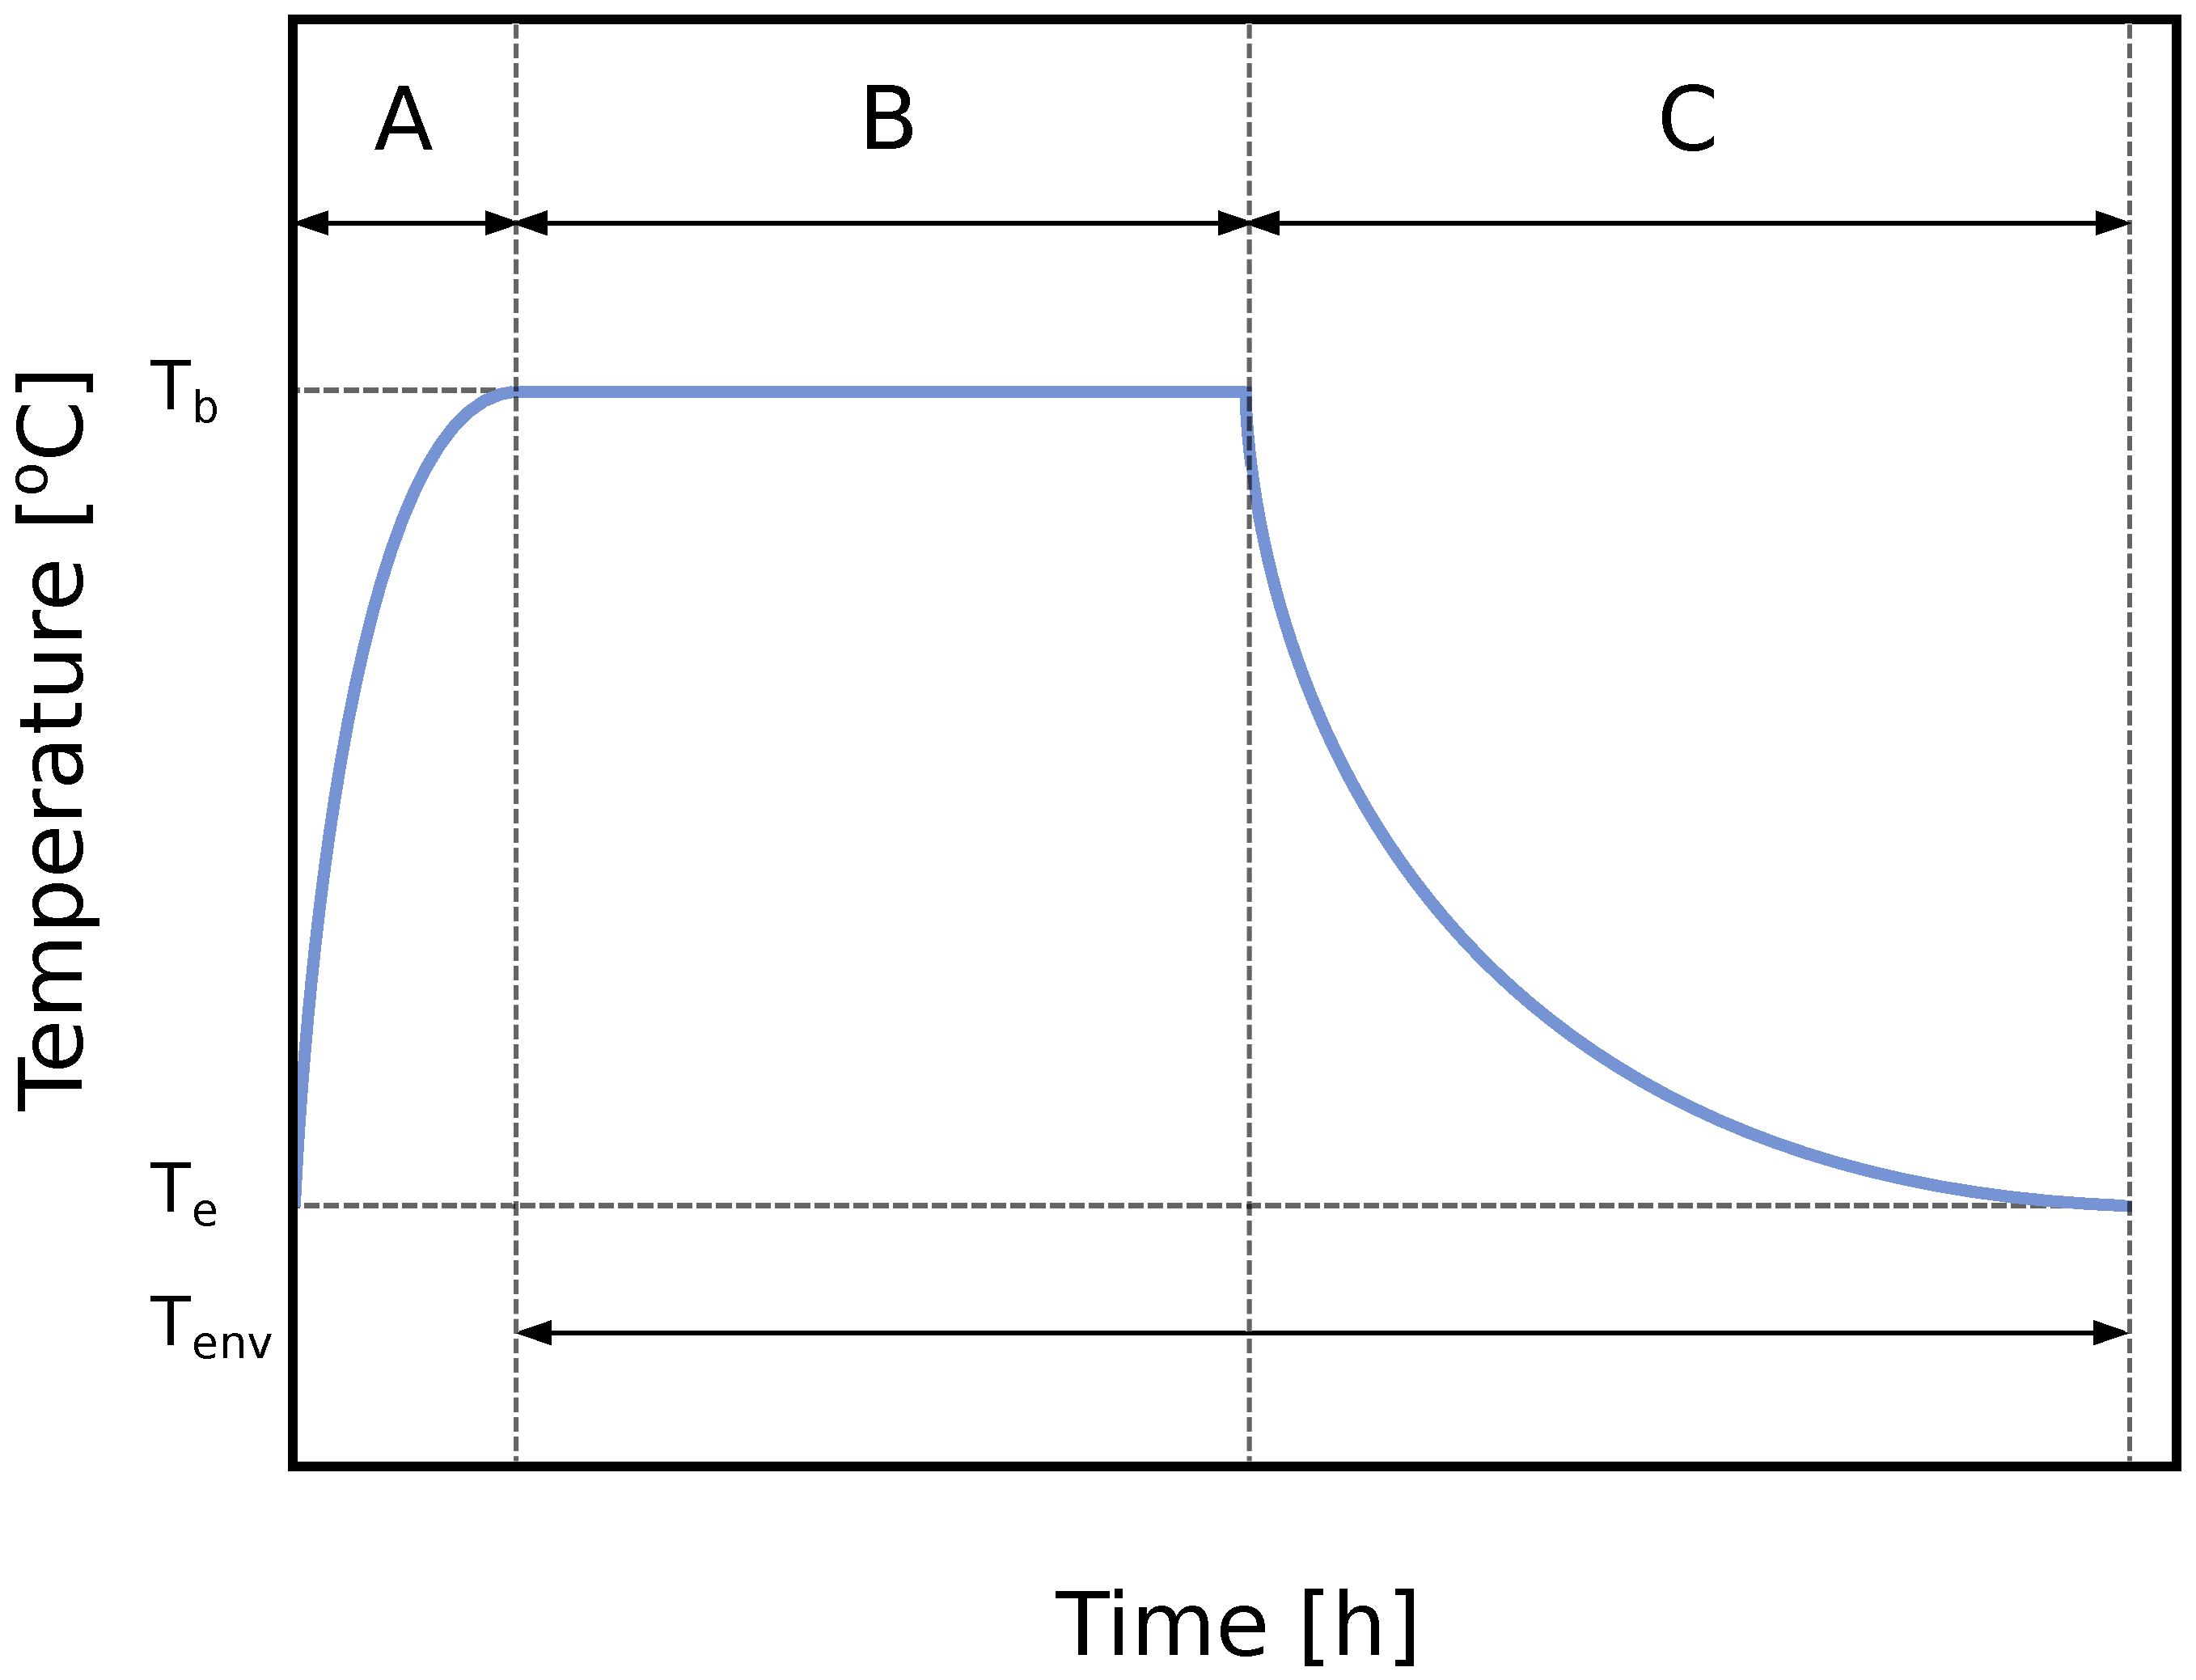
\includegraphics[width=0.63\textwidth]{Pictures/SLS_temp_over_time.eps}\\
        \caption{Phases of an SLS process} 
        \label{fig:SLS_temp_over_time}
    \end{figure}

    As seen in figure \ref{fig:SLS_temp_over_time} \autocites{Inkscape}, the first phase is the time required to reach a specific powder bed temperature $(T_b)$, based on the material of choice. 

    Ideally this temperature should be maintained constant inside the printing
    chamber, during the entire building phase, through infrared or electric heaters. 
    
    The main goal is avoiding drastic temperature gradients in different areas of the printed part, since they can cause 
    visual artefacts such as local or global deformation and, most importantly, uneven residual mechanical tension that can 
    rapidly degrade the structural integrity of the final piece, especially in structural components that might be placed under static or
    dynamic loads. \\ 
    
    Once the final piece is printed, the entire chamber is cooled down homogeneously and gradually, until the equilibrium is reached at room 
    temperature $(T_e)$ \autocite*{Padovano_SLS_Review}. \\ 

    Quality standards for SLS printed parts have increased dramatically over the last few years, to the point where 
    the manufactured components are not exclusively used for prototyping or as sacrificial items for investment casting, but they are 
    used as finalized industrial grade parts. 

    However, there is still room for substantial improvements in the consistency of print accuracy, overall quality, reliability 
    and scalability of the entire process, compared to more traditional manufacturing techniques. \\ 

    The variety of interdepent physical phenomena involved in SLS and their different temporal regimes are the main 
    source of complexity that makes the process inconsistent and very hard to study. 

    The most predominant phenomena are the following \autocite*{Padovano_SLS_Review}: 

    \begin{itemize}
        \item Laser motion and irradiation
        \item Thermal diffusion
        \item Polymer viscous flow and particles coalescence 
        \item Powder spreading
        \item Solidification/crystallization 
    \end{itemize} 
    
    Further improvements are required in order to reduce the amount of discarded parts (still comparatively 
    higher than most consolidated manufacturing techniques), usually defective in terms of porosity or 
    thermal distortion or warping \autocite*{Padovano_SLS_Review}. \\ 

    The next chapters will focus on potential SLS materials for this study and their powder production specifically. \clearpage

    \section{PHAs (Polyhydroxyalkanoates)  \label{PHA_in_general}}

    PHAs are a family of thermoplastic polyesters, obtained by hydroxyalkanoic acids via bacterial fermentation, under 
    nutrient depletion and carbon excess conditions \autocites{Kovalcik_PHA_Review}{Messori_Bondioli_PHAs}. 

    They are a sustainable alternative to petrochemical polymers commonly utilized in 
    additive manufacturing and they are mostly used for prototyping in the medical field \autocites{Kovalcik_PHA_Review}{Messori_Bondioli_PHAs}. 

    Similarly to other sustainable plastics, \textit{PHA} can be produced using industrial byproducts as substrates (corn, soy, coffee, oil wastes, etc.)
    \autocite{Kovalcik_PHA_Review}. \\ 

    The monomer composition of PHA can be very diverse, depending on the microorganisms involved and the fermentation medium. 
    
    This variety impacts the overall mechanical, thermal and chemical properties of the final plastic, which depend on the concentration of 
    different monomers in polymers and copolymers. 

    PHAs can be classified by the chain-length of their monomers \autocite*{Messori_Bondioli_PHAs}: 

    \begin{itemize}
        \item \textit{scl-PHA} (short-chain-length PHA) with 3 to 5 carbon atoms
        \item \textit{mcl-PHA} (medium-chain-length PHA) with 6 to 14 carbon atoms
        \item \textit{lcl-PHA} (long-chain-length PHA) with more than 14 carbon atoms
    \end{itemize}


    Estimating the exact meaningful measures of their properties is not always a straight-forward process, 
    since manufacturers are not transparent about the exact composition of their products, which may have been 
    improved by proprietary additives, whose concentration and exact composition are not usually fully disclosed \autocite{Kovalcik_PHA_Review}. \\ 
    
    The market for bioderived PHA has gradually increased over the years and the growth is estimated to keep its pace, given that not only are they more sustainable
    than competing petrochemical polymers, but they offer additional valuable properties, such as piezolectricity 
    and protection against gases and UV light \autocite{Kovalcik_PHA_Review}.

    Their bio-origin, non-toxicity, renewability, biodegradability and biocompatibility make PHAs a very compelling product in the 
    ever growing market of sustainable materials. 

    However, these desirable qualities contribute to their higher price, which is still not competetive against more established 
    polymers of similar properties \autocite{Kovalcik_PHA_Review}. 

    The increasing demand and the improvements on their biosynthesis will make their price more accessible in the future, for all sorts of 
    applications, including additive manufacturing, where PHAs can be printed successfully either with FDM or SLS techniques. \clearpage

    
    \subsection{PHA and Additive Manufacturing \label{PHA_in_Additive}}

    PHAs can be used in different AM techniques, including Stereolitography, which is part of VP processes \ref{AM_techniques_summary}, 
    FFF (commercially known as FDM), where the filaments are made of a mixture of PHA and PLA, 
    (which increases thermal stability and cuts down cost), and 
    SLS \ref{SLS_general} \autocite{Kovalcik_PHA_Review}. \\ 

    This thesis work focused on its usage in SLS. \\ 

    PHAs have been successfully printed via SLS and utilized in the medical field as scaffolds for tissues engineering applications \autocites{Messori_Bondioli_PHAs}. 

    These scaffolds can be printed with a porous structure (controlled by the laser energy density), 
    which could aid in carrying biomolecules and slowly release drugs, for instance \autocites{Messori_Bondioli_PHAs}.
    
    Unlike with FDM applications, where PHA can not be used as a standalone filament, but needs PLA addition in order to stabilize its melting 
    phase, PHA powders for SLS tend to maintain a better stability and their chemical composition does not get altered as easily. 

    This is a clear advantage, since general properties of the final products do not change drastically from its starting feedstock, 
    and, in addition to this, the remaining powder is not thermally altered in proximity to the melt pool, meaning that it can 
    be reused for additional printing \autocite{Kovalcik_PHA_Review}.  \\
        
    \subsubsection{PHBH \label{PHBH}}

    Poly(3-hydroxybutirate-\textit{co}-3-hydroxyhexanoate) is a copolymer of the PHA family (molecular structure in figure \ref{fig:PHBH_structure}), which gained 
    interest in the AM field and specifically in SLS applications, since it has a wider sintering window \ref{Powder_requirements} than other polyhydroxyalkanoates
    such as PHB and PHBV \autocites{DechetMaximilianA2020OtDo}{doi:10.1063/1.4918516}. \\ 

    \begin{figure}[h!]
        \centering
        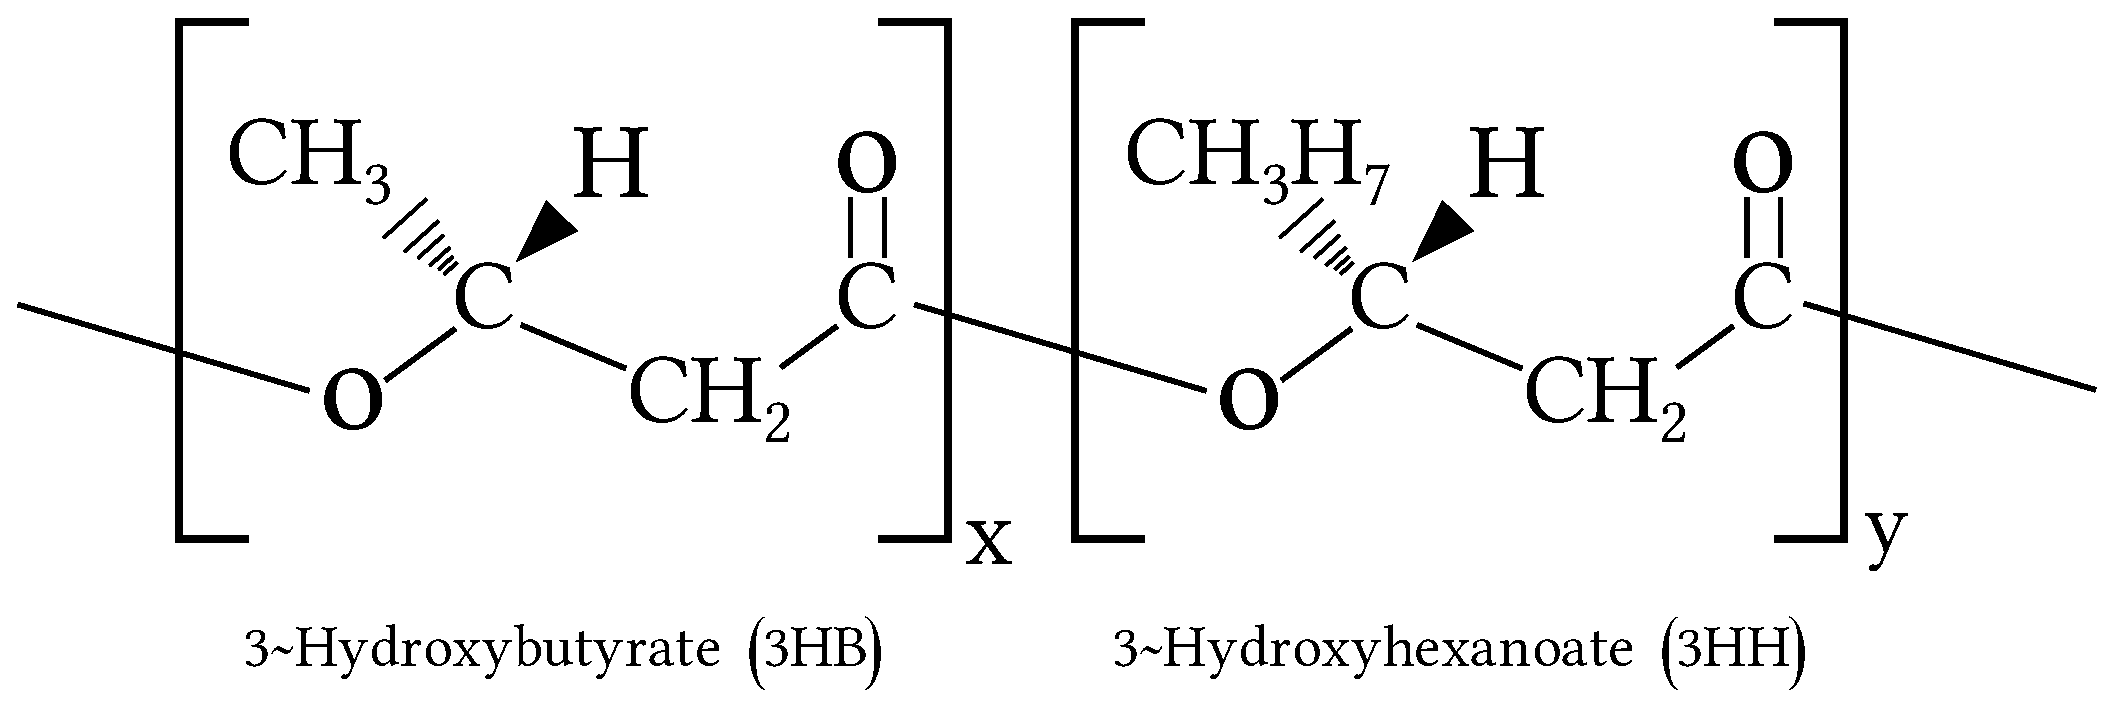
\includegraphics[width=0.8\textwidth]{Pictures/PHBH_chain.eps}
        \caption{Schematic representation of the PHBH polymer structure \autocites{PHBH,Inkscape}.}
        \label{fig:PHBH_structure}
    \end{figure}
    
    Despite having gained attention in the PHA family for SLS, especially in academic environments, the general interest for this copolymer
    is still relatively lower than other 
    petrochemical polymers, due to its early-stage synthesis process, its cost and the strict confidentiality 
    of polymer manufacturers \autocite{Eraslan_PHBH_review}.  

    
    \clearpage

    %\section{PBS (Polybutylene Succinate) \label{PBS_in_general}}
%
    %PBS is an eco-friendly biopolymer, which rose interest among 
    %industrial and academic environments. It possesses excellent properties and major benefits over comparable materials, as well as some minor drawbacks, 
    %which currently hold back its full potential. \\ 
    %
    %While generally brittle, relatively expensive and still challenging to manufacture in SLS-ready powders without compromises on its environmenal 
    %impact (see \ref{Environmental_impact}), this polymer has very desirable features, such as high processability 
    %(with traditional methods, at least), flexibility, as well as visual clarity and specularity. 
%
    %It is also thermally stable and its melting point is around $115 \ \celsius $, which can make its processing, generally speaking, 
    %less energy wasting, especially when mass production is taken into account. 
%
    %PBS is also easy to blend with other materials; for instance, 
    %its mechanical and thermal properties can be drastically improved when used in composite materials, where long or short fibers (or 
    %even particles) can be either randomly distributed, or woven into the polymer matrix.
    %
    %Not only are fibers used for producing high tech composite materials with improved properties, but cheap natural fibers, such as 
    %palm fibers, or even blends with starches, can be utilized as an effective way to cut down cost in 
    %conventional applications, i.e. food packaging \autocite{Rafiqah_Khalina_PBS_review}.
    %
    %
%
%
    %\clearpage
%
    %\section{PBAT (Polybutylene Adipate Terephtalate) \label{PBAT_in_general}}
%
    %PBAT is one of the most promising bio-based polymers in the sustainable plastics market, since it is very eco-friendly and, at the same time, 
    %more performant than comparable alternatives such as PHAs, which exhibit poor mechanical and thermal properties, whereas PBAT is closer to 
    %higher performance petrochemical polymers such as polyethylene terephtalate (PET) and polybutylene terephtalate (PBT) 
    %\autocites*{Jian_PBAT_overview}. \\
%
    %Currently used mainly in food packaging and agriculture, similarly to PBS \ref{PBS_in_general}, PBAT can be blended with other materials, either 
    %for technical enhancing or cost reduction.  
%
    %The considerations made for PHAs and SLS \ref{PHA_in_Additive} should be applicable to both PBS and PBAT, but further experiments need to 
    %be conducted and more reliable data needs to be acquired, although different studies are already showing promising results.  
%
    %\clearpage

    \section{Powder production for SLS \label{Powder_production}}

    Manufacturing raw materials for FDM is a relatively easy process, since the plastics need to be mass produced into filaments or pellets.

    However, producing powders from plastics is a much more convoluted process \autocites{doi:10.1063/1.4918516,Dechet_Schmidt_thermal_rounding,Recent_progress_polymers_AM}. \\ 

    Two radically different approaches are possible, each with its own critical issues: 

    \begin{itemize}
        \item Mechanical milling
        \item Chemical precipitation
    \end{itemize} 

    \subsection{Powder requirements for SLS \label{Powder_requirements}}

    The success rate of SLS prints is highly dependent on the characteristics of the powders involved. 

    The key factors in powder quality are particle size distribution, morphology, as well as thermal, flow and optical properties. \\
    
    Ideally, a gaussian distribution, with most particles close to the average size is desirable, 
    with a tipical range of $(20 \div 80) \ \mu m$ \autocite*{doi:10.1063/1.4918516}. 

    The average particle size directly influences the layer thickness in the SLS process.  
    
    Powder morphology is crucial in the sintering mechanism, where regular, smooth and non-hollow spherical 
    particles are preferrable in order to effectively obtain sintering necks, as illustrated by figure \ref{fig:SLS_sintering_neck} \autocite*{doi:10.1063/1.4918516}.  

    \begin{figure}[h!]
        \centering
        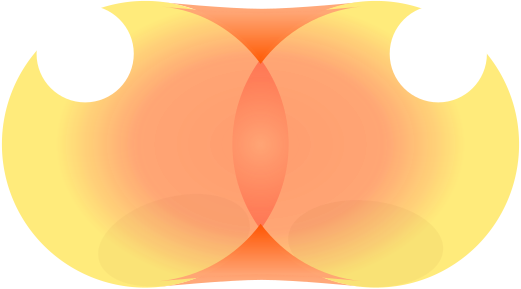
\includegraphics[width=0.45\textwidth]{Pictures/sintering_neck.eps}\\
        \caption{Two spherical powder particles forming a sintering neck \autocite{Inkscape}} 
        \label{fig:SLS_sintering_neck}
    \end{figure}

    The powder's density is another parameter that should be considered, as it directly correlates with the final part's 
    global density and it allows calculation of the Hausner ratio $H_r$ (as seen in equation \ref{eq:Hausner_ratio}), which is a direct predictor of powder flowability. 
    
    Ideally, this coefficient should be lower than 1.4, otherwise the powder could result in issues with fluidization \autocite*{doi:10.1063/1.4918516}. 

    \begin{equation}
        H_r = \frac{\rho_{tap}}{\rho_{bulk}}
        \label{eq:Hausner_ratio}
    \end{equation} 

    where $\rho_{tap}$ is the tap density and $\rho_{bulk}$ is the bulk density of the powder. 

    \clearpage



    Understanding thermal properties of the powder is essential in SLS. 


    SLS is characterized by an optimal sintering window, with a temperature range between
    crystallization $(T_c)$ and melting $(T_m)$. 
    For any given heat flow within that range, the material is in a metastable phase, 
    where full coalescence of the top powder layer, as well as adhesion with previously sintered layers are 
    most likely guaranteed \autocite{doi:10.1063/1.4918516}. 

    Therefore, creating a tailor-made powder feedstock involves using materials with a wide enough 
    sintering window \autocites*{DechetMaximilianA2020OtDo}{doi:10.1063/1.4918516}. \\

    Furthermore, optical properties of the powder bed need to be taken into account, since highly reflective materials (for a given 
    laser wavelength) can waste most of the energy input, instead of absorbing a significant amount of radiation needed to 
    effectively melt the powder \autocite{doi:10.1063/1.4918516}.  

    This issue is prevalent in metal SLM \ref{SLS_general} \autocites{Latvian_additive}. 
    
    However, when it comes to SLS and plastics powders, the required energy is substantially lower than that needed to melt metal alloys, 
    meaning that any potential problem with poor radiation absorbtion can be compensated by increasing the 
    laser power output \autocite{doi:10.1063/1.4918516}. \\ 
    
    Viscosity and surface tension of the melt pool are more relevant factors when choosing powders for SLS. 
    High viscosity and surface tension can hinder the coalescence of polymer powders and the adhesion with previously 
    sintered layers, resulting in residual sheer stress, high porosity and thus poor quality of the 3D printed part in general. 
    
    In SLS, unlike other processes i.e. investment casting or injection molding, there is no well distributed force
    (e.g. built up pressure against the mold) that can increase particle coalescence and layer adhesion. The only relevant
    force acting on the printed part is gravity, along the vertical axis \autocite*{doi:10.1063/1.4918516}. 

    \subsection{Mechanical milling \label{Mechanical_milling}}

    Grinding plastics into fine and homogeneous powders can be a challenge, since the high speed milling devices can easily overheat the 
    plastics above their softening point, creating lumps of material, far from the desired result.
    
    A solution to this problem is using so called \textit{cryogenic grinding} devices, which utilize cooling agents such as dry ice, liquid 
    carbon dioxide or liquid nitrogen, in order to keep the plastics below the glass transition point, where polymers become intrinsically
    brittle, similarly to a ceramic material, making it possible to turn the original mass into a powder \autocites*{cryogenic_grinding_video}{Junghare_cryogenic_grinding_review}. 

    The heterogeneous powders can later be sieved and separated, based on their different granulometry. \\ 

    Despite being an effective process for powder production, the morphology obtained with cryogenic milling is extremely irregular 
    and unpredictable, which makes this method generally unsuitable for high quality SLS parts \autocite*{doi:10.1063/1.4918516}. 

    \subsection{Chemical precipitation \label{Chemical precipitation}}

    There is little variety in the market of SLS ready polymer powders, with polyamide-12 (PA12) being the most optimized for this 
    application and being produced by precipitation in ethanol \autocite*{DechetMaximilianA2020OtDo}.
    
    Many other polymer powders can be produced using the precipitation method, but their development is currently very limited 
    and in early-stage, especially with thermoplastics, which are not as optimized as PA12.
    
    Most of the experimental work on the precipitation method for thermoplastics is not made available by large chemical corporations, 
    but rather by academic environment. 

    \subsubsection{Polymer-Solvent System \label{polymer_solvent_system}}

    Assuming there is a potential material to use this technique with, the recommended solvent choice gravitates towards 
    so called \textit{moderate solvents}. \\
    
    These compounds have the peculiarity of acting as a solvent only when heated above a certain temperature. 

    Therefore, thermoplastics can be dissolved into a compatible solvent and form a liquid-liquid phase separation
    upon cooling of the system, where complex crystallization and precipitation phenomena are later induced via stirring of 
    the nucleated polymer-rich droplets \autocite*{DechetMaximilianA2020OtDo}.  \\ 

    A common criterion of solvent pre-selection is the evaluation of Hansen parameters, through the following equation: 

    \begin{equation}
        \textit{f} (\delta_x) = 100 \cdot \frac{\delta_x}{\delta_d + \delta_p + \delta_h}
        \label{eq:hansen_parameters}
    \end{equation}

    which quantifies the interaction between the polymer and the solvent, in correlation with the dispersion $(\delta_d)$, 
    the polar interactions $(\delta_p)$ and the hydrogen bond interactions $(\delta_h)$ \autocite*{DechetMaximilianA2020OtDo}. 

    Once the polymer-solvent system is tested, the experimental data can be effectively represented in the TEAS plot (as shown in figure \ref{fig:TEAS_plot}), which 
    helps visualizing the equation (\ref{eq:hansen_parameters}). 

    \begin{figure}[h!]
        \centering
        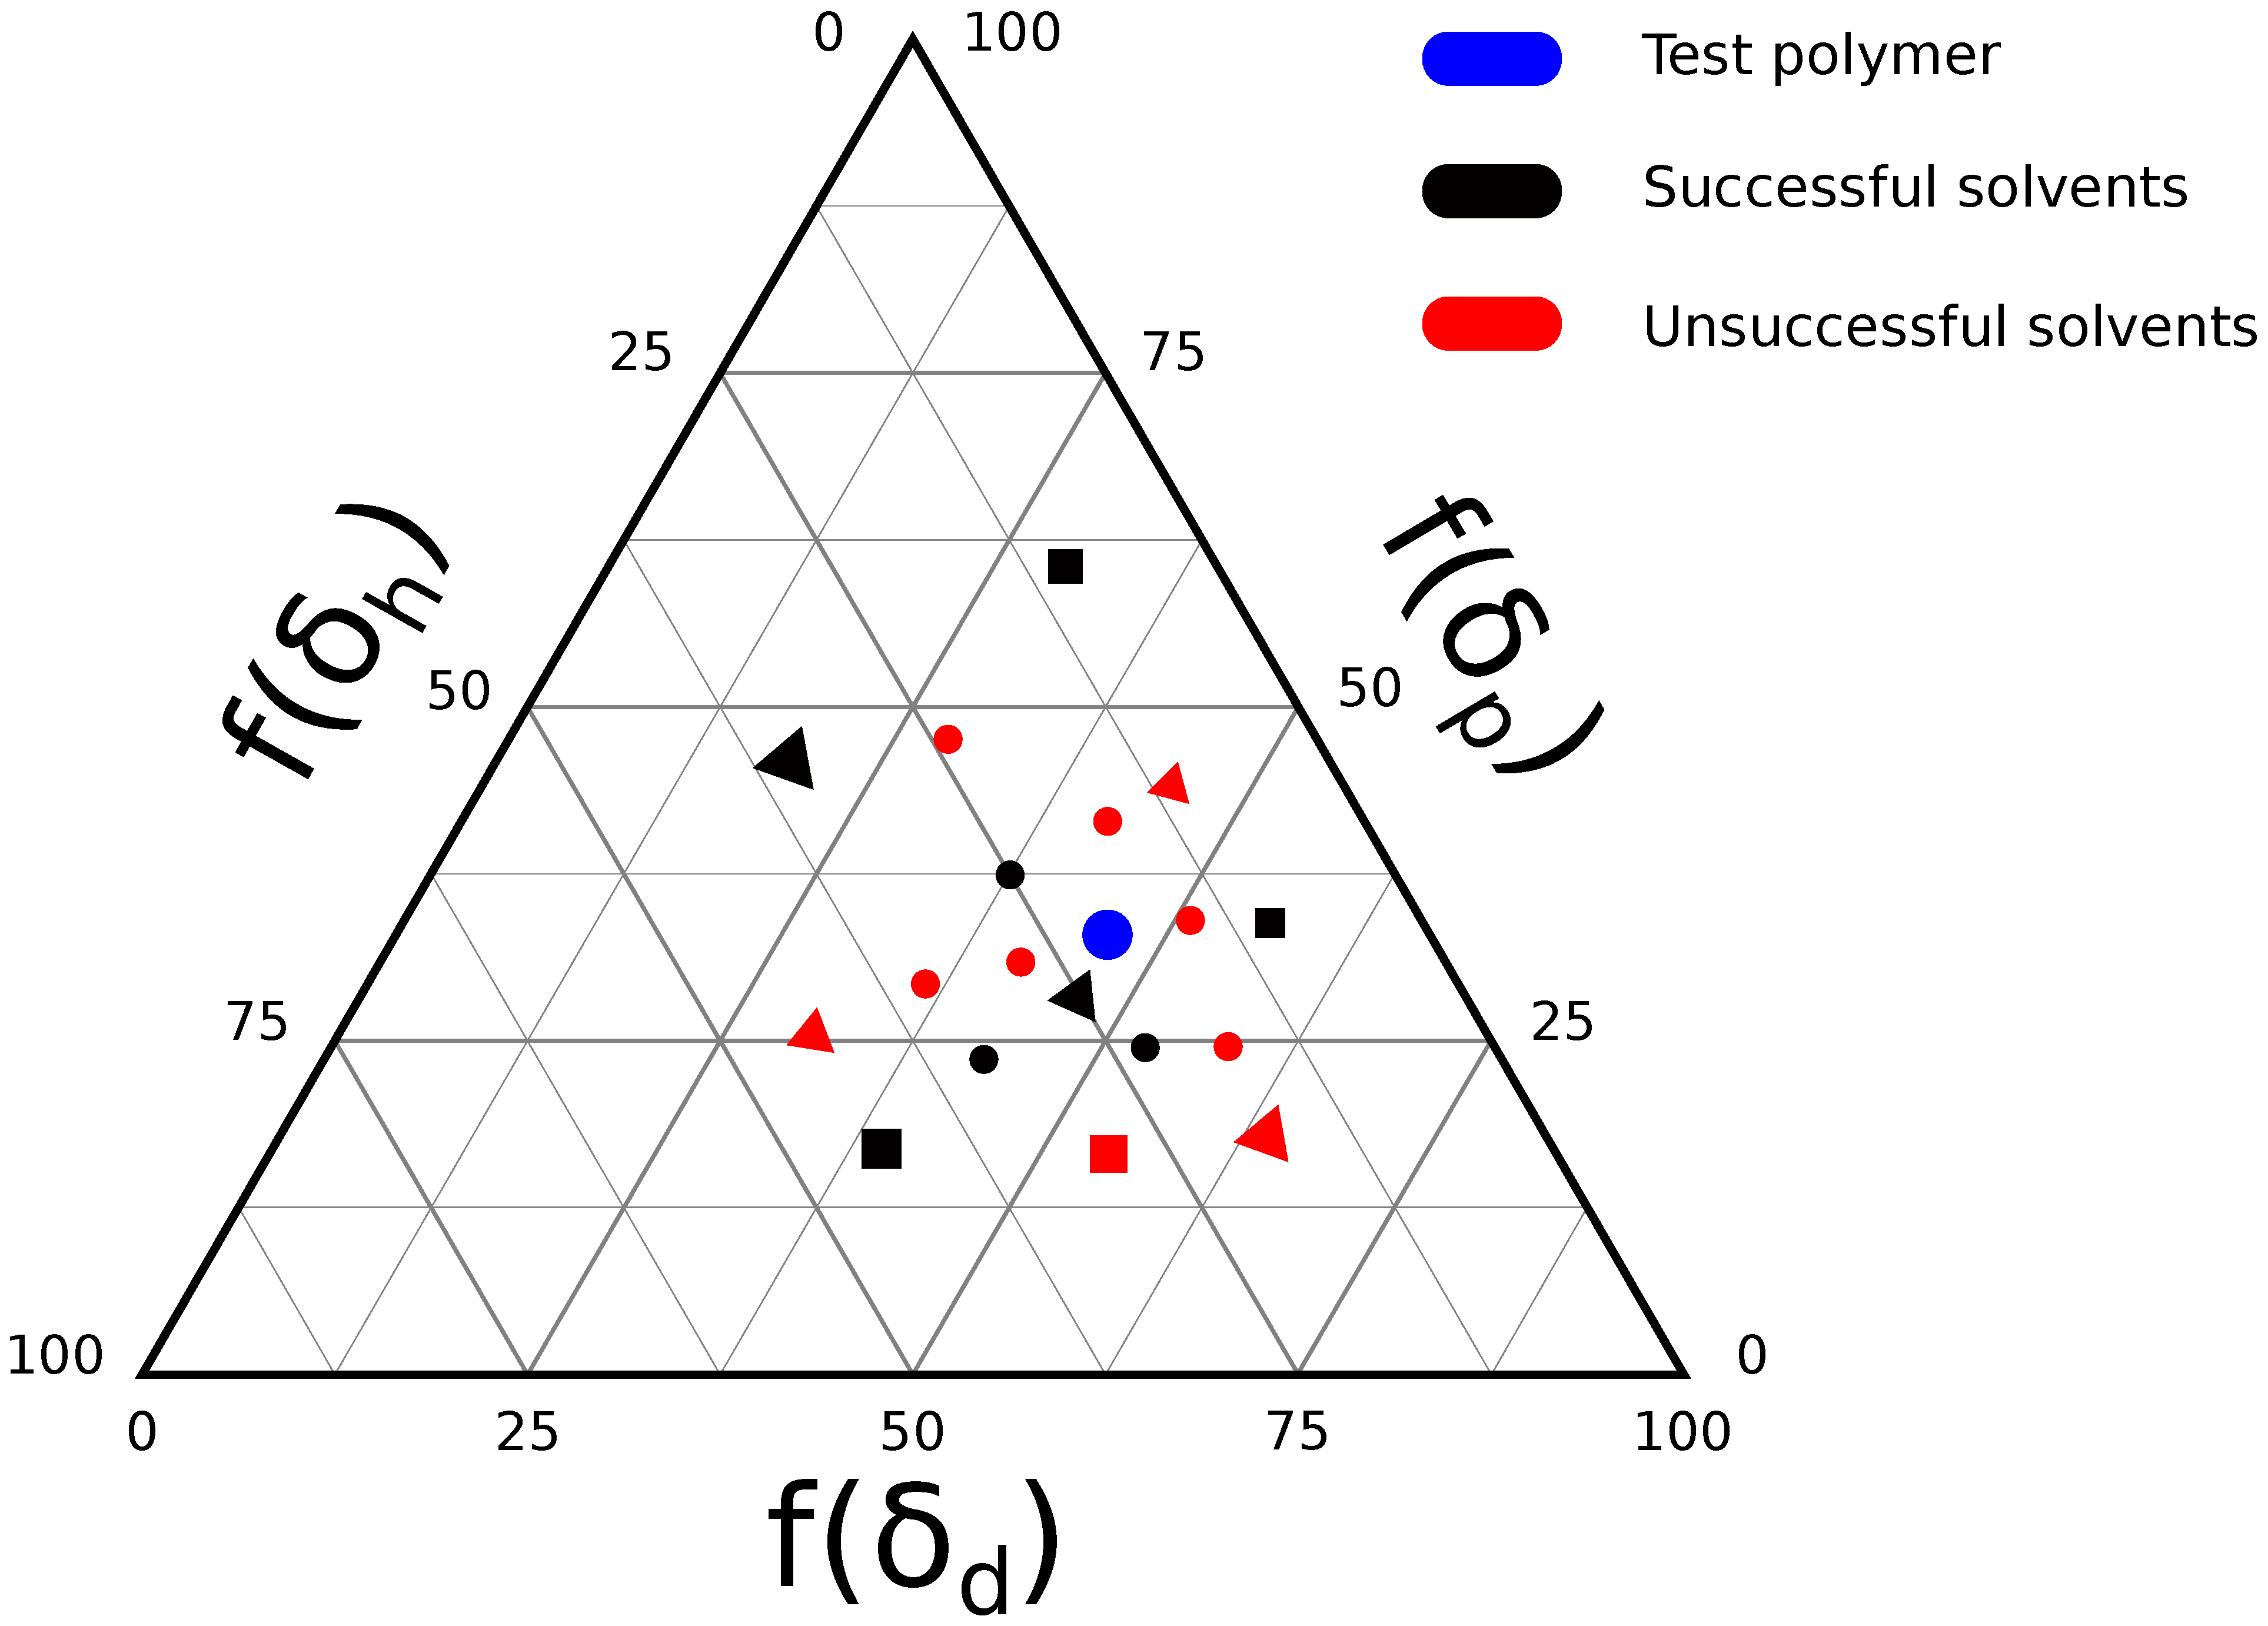
\includegraphics[width=0.4\textwidth]{Pictures/TEAS_plot.eps}
        \caption{Generic TEAS plot for any given polymer \autocites{DechetMaximilianA2020OtDo}{Inkscape}}
        \label{fig:TEAS_plot}
    \end{figure}


    This approach has been successfully used to determine solubility of PP (\textit{polypropylene}), PET (\textit{polyethylene terephthalate}), 
    PC (\textit{polycarbonate}), etc, and could be effectively utilized with bio-based polymers such as PHBH \ref{PHA_in_general}.
    
    

    \subsubsection{Cloud point diagram \label{Cloud_point_diagram}}

    After choosing a suitable moderate solvent, the process needs to be studied and quantified 
    with a cloud point diagram of temperature, as a function of polymer weight concentration, allowing the identification of a dissolution 
    temperature and the temperature where LLPS (liquid-liquid phase separation) occurs. 
    
    These measures allow better scalability of the process in larger controlled environments such as a reactor or autoclave system \autocite{DechetMaximilianA2020OtDo}.
    
    \subsubsection{Production in a controlled environment \label{precipitation_production_controlled_environment}}

    The cloud point diagram data allows for an optimization of the production process in autoclave or reactor system. 

    Temperature profile, initial polymer concentration and, most importantly, stirring conditions can greatly influence the final 
    particle size distribution. 
    
    Stirring is the most impactful of these factors, producing smaller particles as the intensity increases \autocites{DechetMaximilianA2020OtDo}, as reported in figure \ref{fig:stirring_rpm}. 

    \begin{figure}[h!]
        \centering
        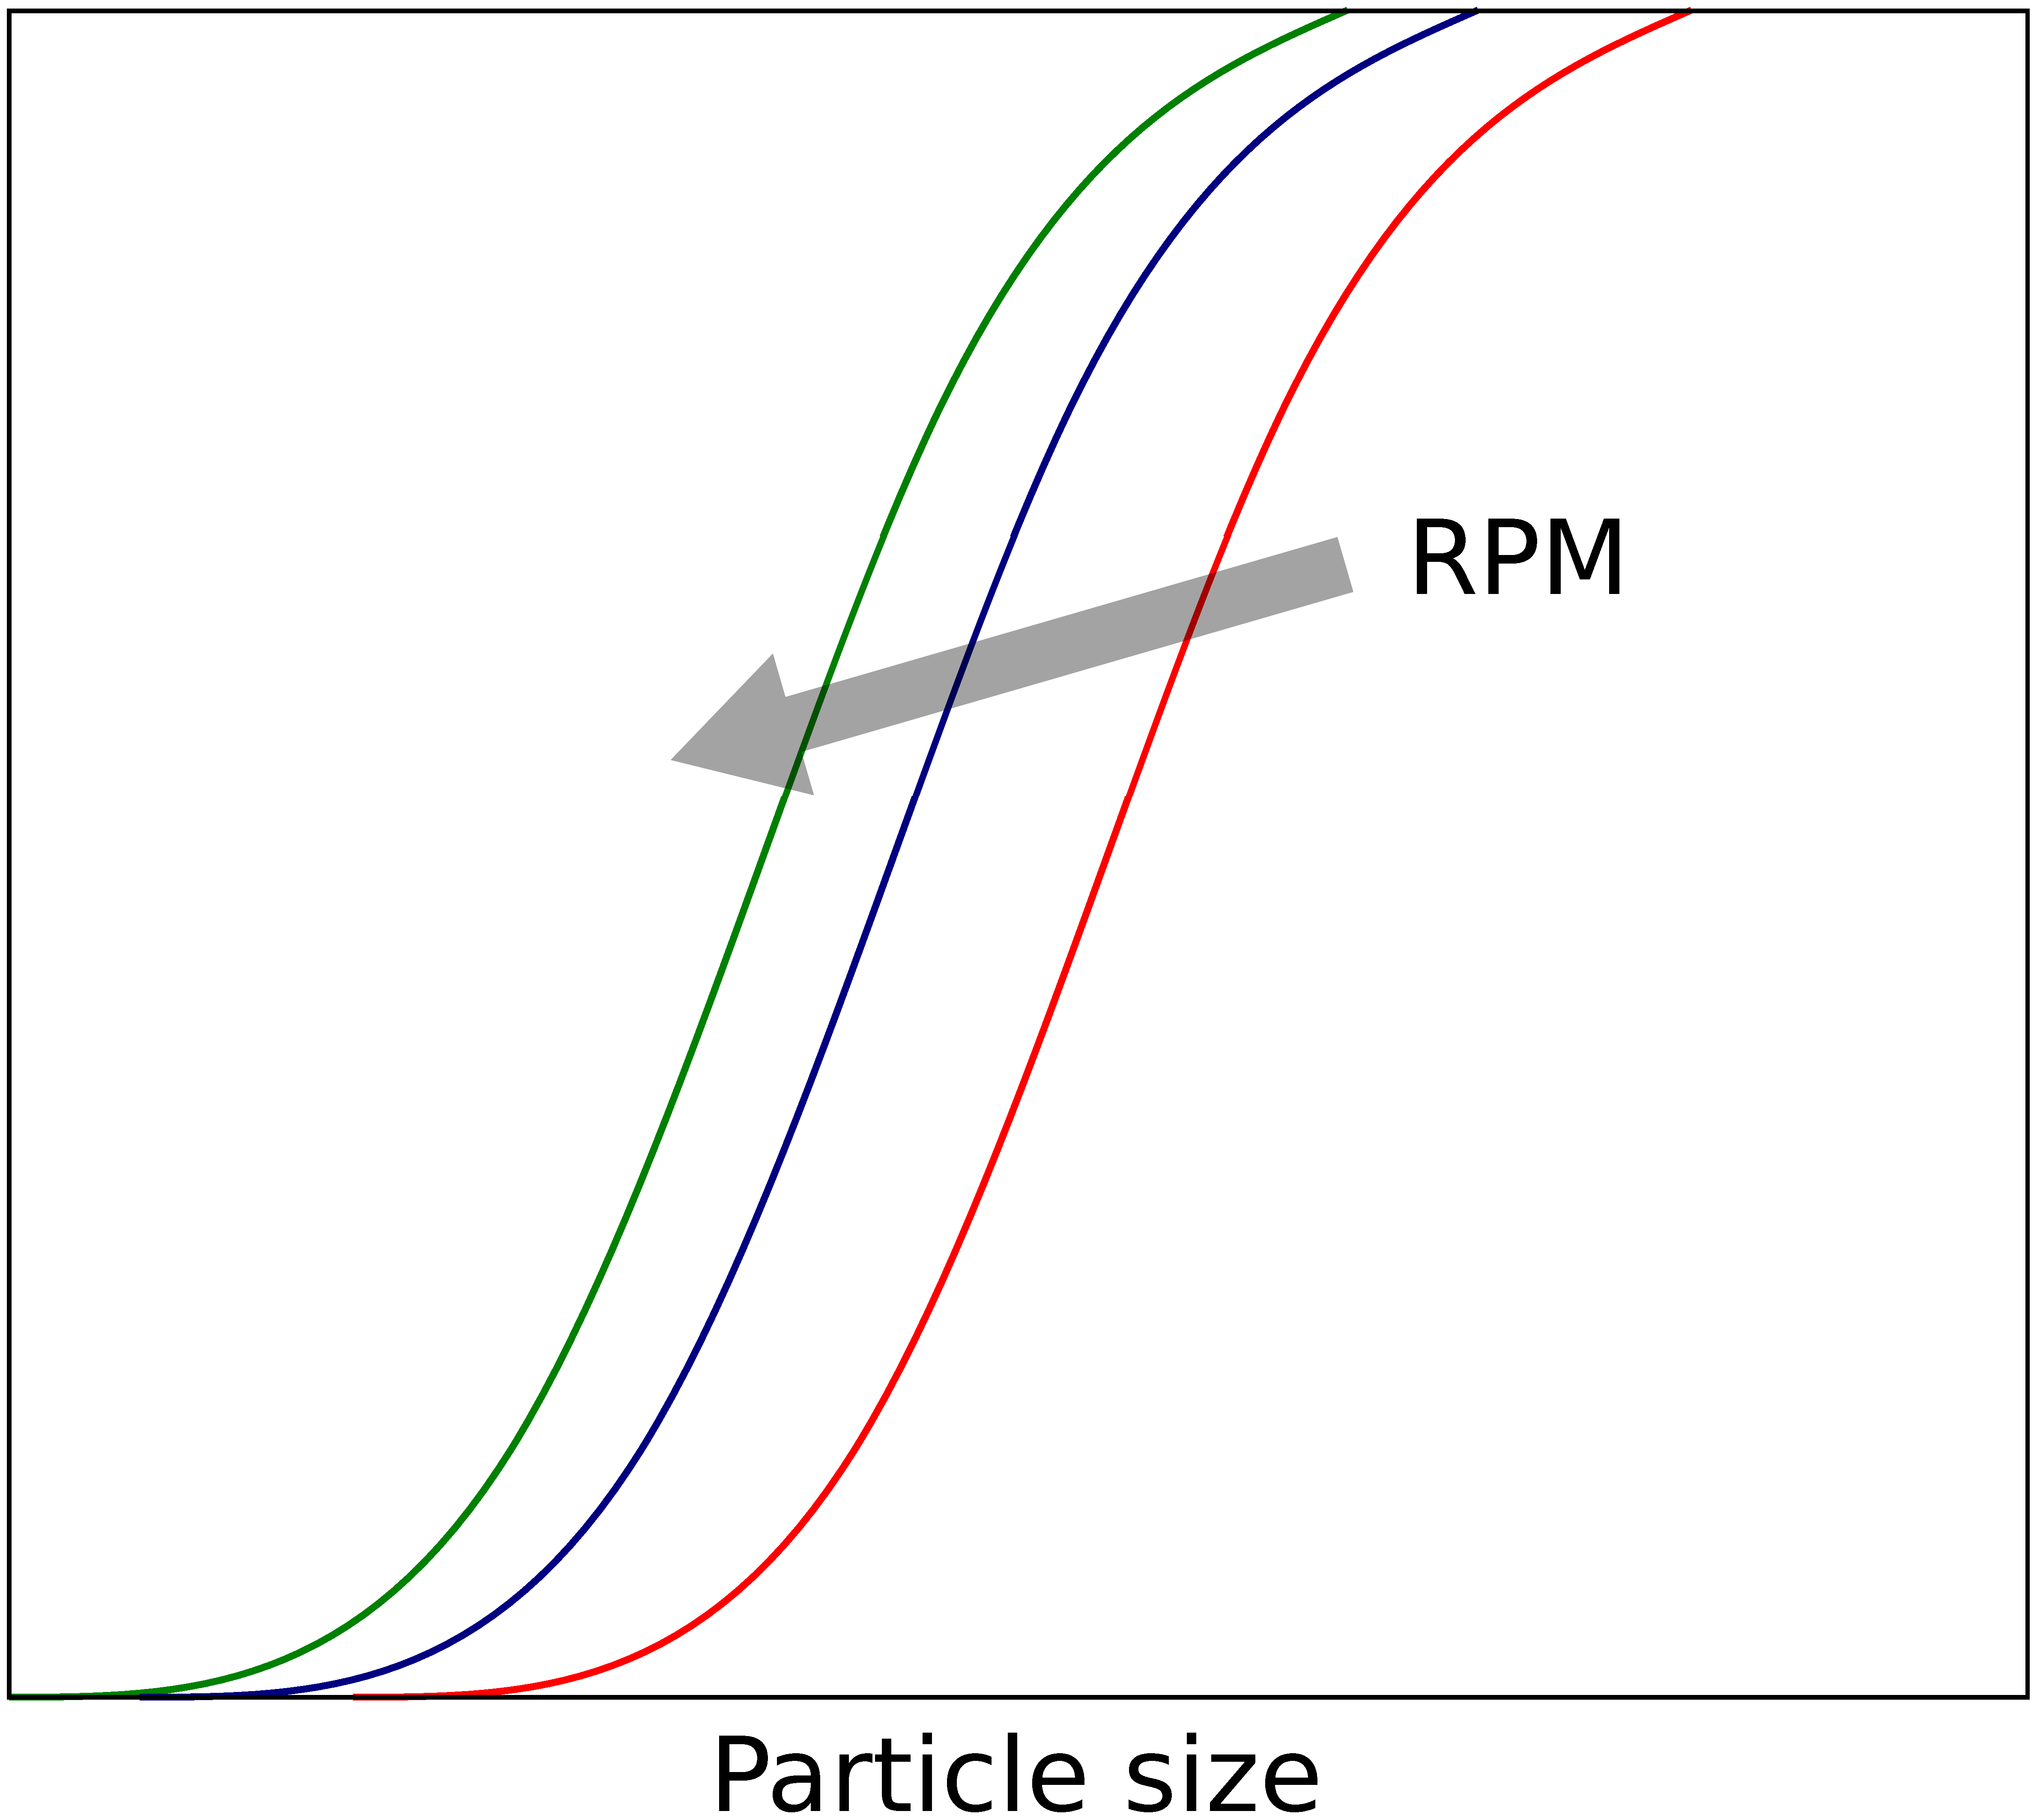
\includegraphics[width=0.5\textwidth]{Pictures/particle_size_stirring.eps}
        \caption{Particle size decreases as stirring RPM increase \autocites{Inkscape}}
        \label{fig:stirring_rpm}
    \end{figure}

    \subsection{Environmental impact \label{Environmental_impact}}

    At first glance, cryogenic milling seems to be a more sustainable option for powder production. However, the issues discussed in \ref{Mechanical_milling}, 
    make this method unsuitable for SLS, unless future development will improve overall powder morphology, perhaps with the aid of 
    post processing via thermal rounding of the particles \autocite{DechetMaximilianA2020OtDo}. \\ 
    
    On the other hand, while powder production by 
    chemical precipitation produces much better and more 
    controllable powder feedstock, it is worth noting that organic solvents are intrinsically environmentally impactful and that should be taken 
    into account, especially for large scale production of these powders. 

    The entire purpose of utilizing sustainable bio-based polymers in the first place might be rendered pointless, if their powder production 
    utilizes compounds or processes that are not environmentally friendly. \\ 

    Better innovative solutions (or mitigations of the mentioned issues in the current pipelines) need to be implemented in the near future. \\ 

    Thermal rounding is a heat treatment, aimed at improving the bulk powder morphology for SLS applications. 
    This kind of treatment might be the crucial step in the success of a more environmentally friendly pipeline, which does not involve 
    any polluting solvent.

    Powders can be heated either directly, with a carrier gas, or indirectly, using heated walls. 

    While the former method has a better process yield and reduced risk of lumping, the latter produces powders with 
    a better, more spherical morphology, but with a significantly higher risk of particle agglomeration \autocite{Dechet_Schmidt_thermal_rounding}.

    \clearpage

    %\section{Laboratory environmental conditions and available equipment\label{Lab_condition_equipment}}
%
    %The experimental phase of this case study has been conducted in various laboratories at \textit{DISAT@PoliTo}. \\ 
%
    %The main production process (\ref{Choice_material_process}) has been studied and optimized in 
    %a dedicated lab, then the residual moisture of each - cleaned and 
    %unsieved - batch of powder has been removed by oven drying (\ref{Choice_material_process}).
%
    %Several powder samples, collected at different phases of the optimization process, have been analyzed 
    %with a \textit{SEM} (Scanning Electron Microscope) at a third party 
    %facility (\ref{SEM_analysis}), and subjected to 
    %a \textit{TGA} (\ref{TGA_Analysis}) and a \textit{DSC} (\ref{DSC_analysis}) 
    %at the \textit{Thermal Analysis} lab of the same department. \\ 
    %
    %The laboratories are equipped with a large workbench and are stocked with all sorts of useful tools and equipment, especially flasks,
    %beakers and glassware 
    %in general, as well as a chemical hood, which is essential for a safe use of chloroform 
    %(\ref{Initial_recipe}, \ref{detailed_reaction}). \\ 
%
    %The extremely high summer temperatures and humidity were environment conditions that had to be taken into account, 
    %especially when working with chloroform, which is a highly volatile compound. \\
%
    %These potential issues have been addressed as later explained in detail, with adaptations and better choices among the available pieces of
    %equipment (\ref{recipe_improvement}, \ref{faulty_equipment}), as well as tweaking of the precipitation 
    %reaction, which in turn increased the pellet-to-powder yield by over ten-fold, compared to the initial 
    %results (\ref{initial_failures}).



    \clearpage
    \section{Choice of material and production process\label{Choice_material_process}}

    As seen in previous chapters \ref{PHBH}, \ref{Powder_production}, this thesis work focused on PHBH, mainly for its wider sintering window, among all PHAs. \\ 

    An early stage precipitation reaction had already been developed for PHBH, by other teams involved in the research. 
    This initial recipe has been tested out with the other bio-based polymers as well, but PHBH held the most promising 
    results even in its early stages. \\ 

    Other approaches such as cryogenic milling \ref{Mechanical_milling} have been taken into consideration, but quickly 
    discarded, due to the lack of equipment suitable for thermal rounding treatments. 

    The grinding procedure, aided by liquid nitrogen, proved to be successful at producing fine powders, according to the literature \autocites{Dechet_Schmidt_thermal_rounding}. 

    However, unless a thermal rounding treatment is applied, the powder 
    morphology is too irregular and far from the ideal spherical geometry, thus making the 
    obtained batches unsuitable for 3D printing. \\  

    All of the mentioned points led to definitely choosing PHBH for this thesis work, focusing on the optimization of 
    the available blueprint for a suitable chemical 
    precipitation process, as explained in the following chapters \ref{Initial_recipe}, \ref{detailed_reaction}, \ref{recipe_improvement}. 

    \clearpage
    \section{Initial chemical precipitation recipe for PHBH\label{Initial_recipe}}
    
    As mentioned earlier, a prototype for a chemical precipitation reaction had already been developed, 
    derived from experiments on solute-solvent compatibility (see figure \ref{fig:TEAS_plot}), 
    which highlighted a good affinity between PHBH and chloroform. \\ 

    Starting from a 4 g batch of PHBH pellets, the highest amount of sieved powder ($ < \ 100 \ \mu m$ )
    ever produced was around 1.2 g, resulting in a $30 \ \% $ maximum yield. \\ 

    The very early experiments were conducted using a trial and error approach, with the issues previously discussed 
    playing a major role in the reaction's rate of success. 
    
    The environmental conditions at the time were drastically different compared to those experienced during the latest experimental 
    activities. 

    Most importantly, the lab temperature was substantially lower, as the reaction was prototyped during winter. 
    
    As earlier mentioned, the extremely high summer temperatures dramatically increased the evaporation rate of 
    chloroform, leaving a high viscosity solution that was harder to control during precipitation. \\

    This led to failures and practically insignificant yields (as explained in section \ref{initial_failures}) if 
    the reaction succeeded, when testing the recipe in these conditions.  

    After thoroughly studying the process in all its phases and isolating different variables that could have caused the issues, 
    the recipe has been tweaked and adapted to the external conditions, which is later discussed 
    in \ref{recipe_improvement}, \ref{key_variables}. 

        \subsection{Materials\label{Components}}

        The ingredients and quantities of the prototype reaction were the following: 

            \begin{itemize}
                \item 4 g of PHBH pellets 
                \item 55 ml of chloroform 
                \item 400 ml of $0.25 \ \% $ (by weight) of PVA solution 
            \end{itemize} 
        

        Despite its apparent simplicity, the reaction is highly influenced by the environmental conditions, as well as
        equipment's correct use and proper operability. \\ 
        
        Any slight deviation from the correct parameters, whether due to 
        unpredictable changes in environmental conditions, malfunctioning or incorrect use of the available tools, could 
        in fact potentially break the unstable equilibrium of the reaction, making it extremely 
        hard to pinpoint the exact root cause of failure. \\  

        Several failed attempts, changes in equipment and tools, as well as quantities were required in order 
        to understand the most relevant parameters of the entire process. 
        \clearpage
        %\subsection{Equipment\label{Equipment}}
%
        %All the essential pieces of equipment and tools for the reaction are listed here: 
%
        %    \begin{itemize}
        %        \item Clean flasks and glassware for volumetric measurements, waste containment and disposal, etc
        %        \item A high precision weight scale 
        %        \item A magnetic stirrer and heater 
        %        \item Appropriately sized stir bars \footnotemark 
        %            \footnotetext{An inadequate stir bar size, in comparison to the stirring container, can 
        %            be unstable and stop stirring or create undesired foams and splashes}
        %        \item Appropriately sized beakers for the PHBH-chloroform and the PVA solution \footnotemark 
        %            \footnotetext{An adequately sized and shaped container is required for the same reason}
        %        \item A flow controllable dripper 
        %        \item A chemical hood \footnotemark
        %            \footnotetext{A chemical hood is generally required to safely operate with chemicals that produce 
        %            vapours or fumes. Chloroform evaporates extremely quickly and is mildly toxic. Suddenly inhaling 
        %            a large amount can cause a human to lose consciousness}
        %        \item Distilled water for powder and tool cleaning 
        %        \item A vacuum ejector 
        %        \item A fritted glass filter or a paper filter \footnotemark
        %            \footnotetext{A porous filter combined with a vacuum ejector is preferred, as it 
        %            exponentially decreases powder filtering and cleaning time} 
        %        \item An oven or dehydrator
        %        \item A sieve \footnotemark
        %            \footnotetext{A ($ < \ 100 \ \mu m$ ) sieve was available, but smaller 
        %            sizes ($20\div 80 \ \mu m$) could be required}
        %        \item Sealed test tubes or any other container suitable for fine powders storage \footnotemark
        %            \footnotetext{Electrostatic attraction to different materials can cause significant powder losses over time}
        %    \end{itemize}
%
%
        %\clearpage



        \subsection{Detailed step-by-step reaction\label{detailed_reaction}}

        The reaction is shortly described by the following diagram: 

            \begin{figure}[h!]
                \centering
                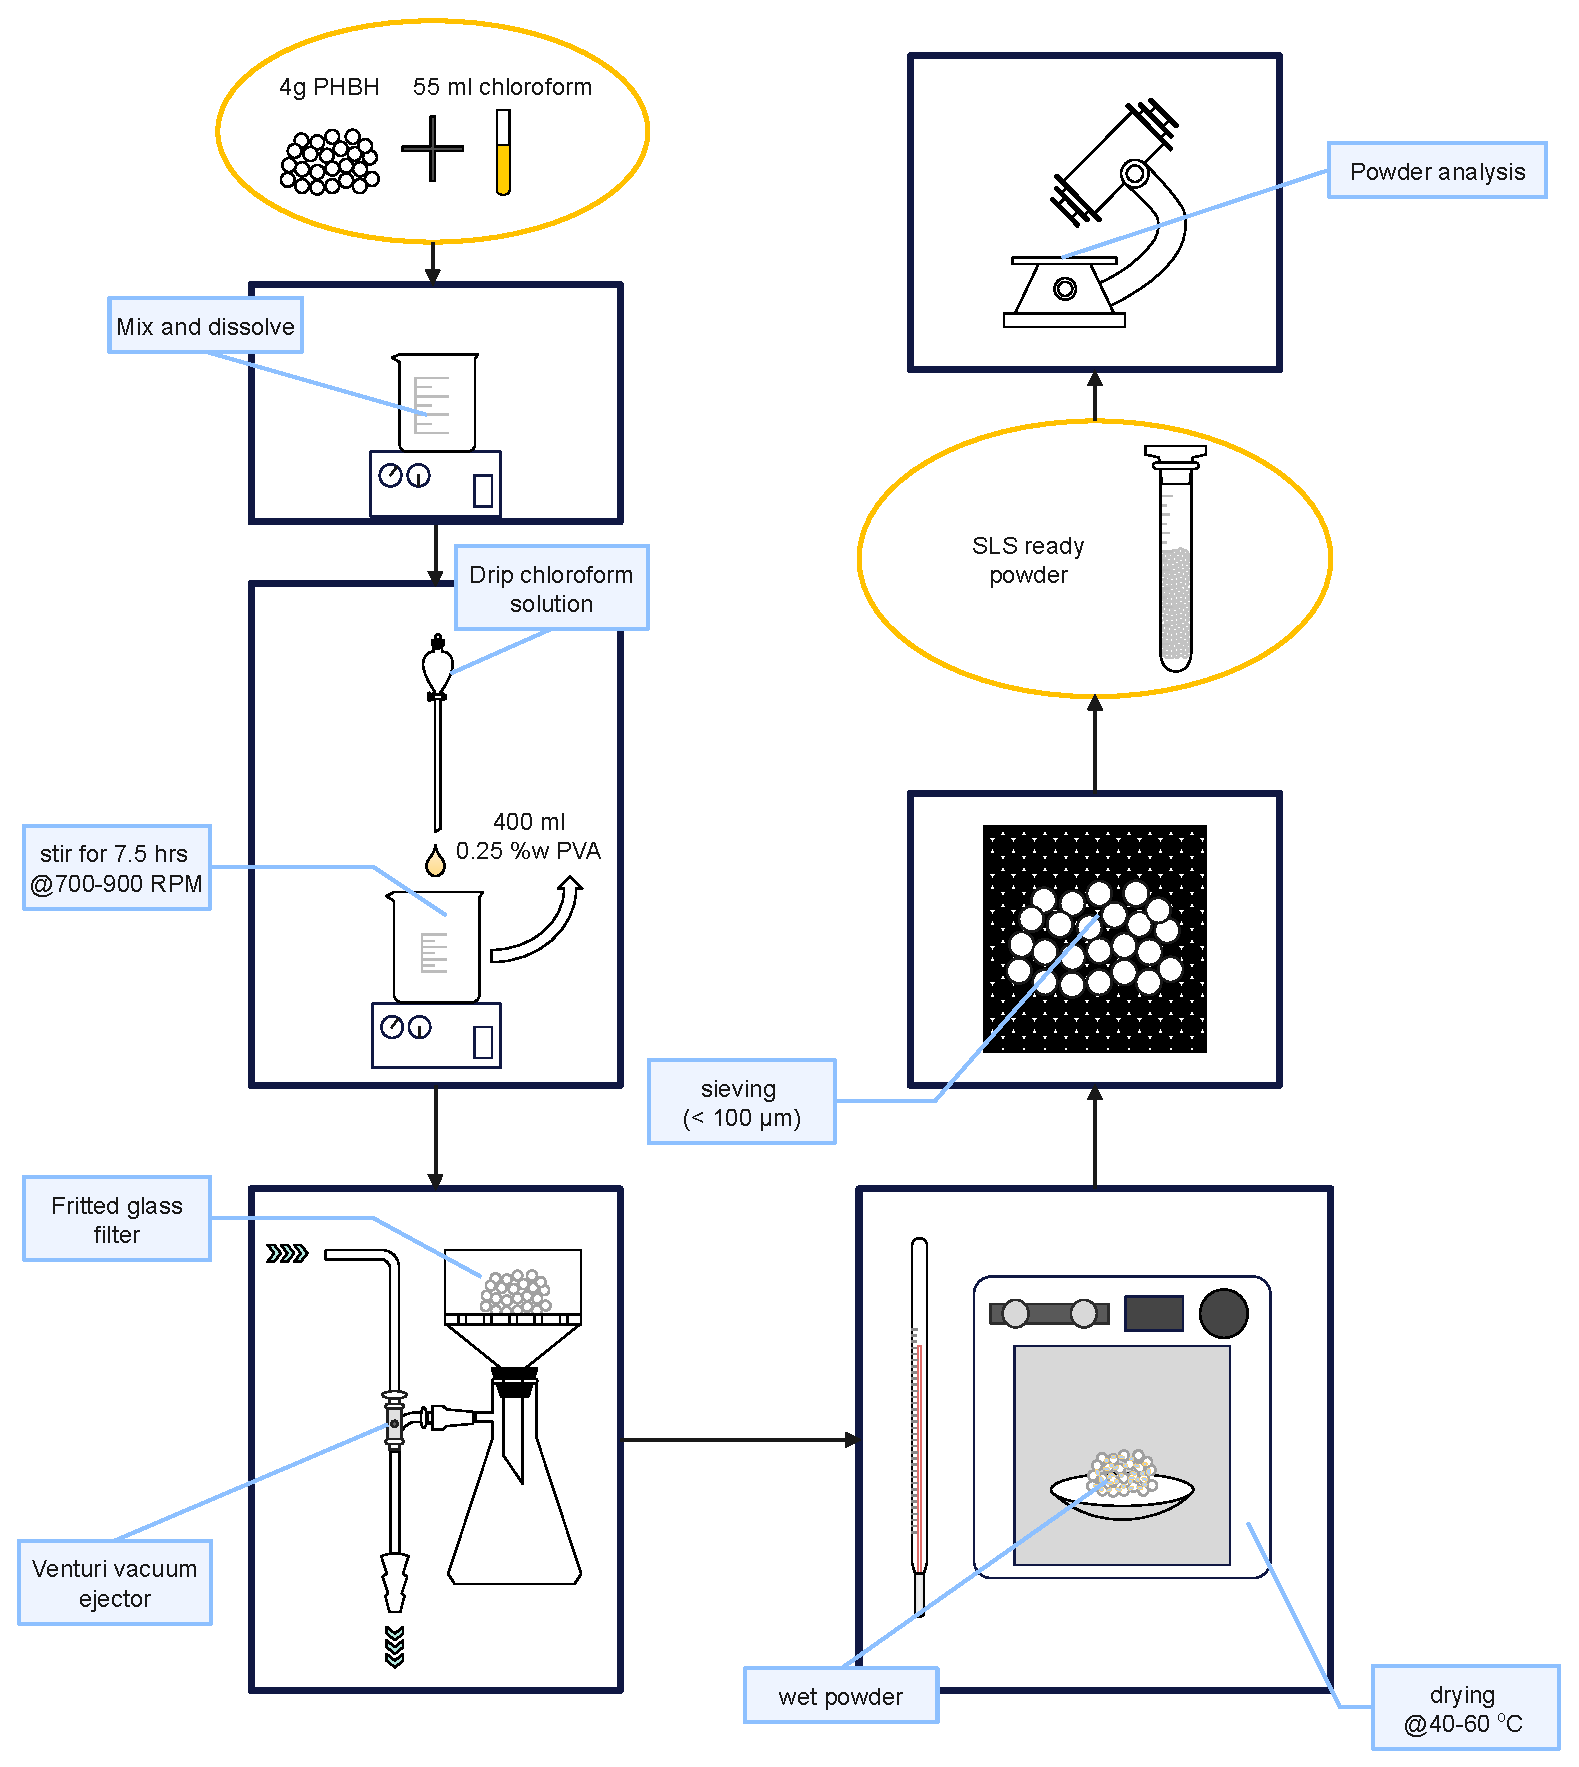
\includegraphics[width=\textwidth]{Pictures/process_diagram.eps}
                \caption{Process diagram describing the entire powder production pipeline \autocite{Inkscape}}
                \label{fig:process_diagram}
            \end{figure}

        \clearpage

        PHBH pellets (4 g) were dissolved into 55 ml of chloroform, in order to create a viscous liquid that has later been slowly dripped into a 
        $0.25 \ \%$ PVA solution, where the precipitation phenomenon occurred for a duration of 7.5 hours, at 700 rpms. \\ 

        %Depending on the recipient used to contain the viscous solution, the stir bar should be appropriately sized and 
        %the stirring speed should be adjusted accordingly, in order to minimize evaporation and avoid the formation of foams and 
        %splashes of chloroform. \\ 
        
        It is important to highlight that way too low speeds can result in a long stirring time and excessive evaporation of chloroform, which leads to 
        higher viscosity and issues with the formation of fine powders during precipitation, as previously discussed. \\ 

        On the other hand, splashes and foaming can occur at excessively high stirring speeds, causing loss of liquid, or
        hindering the visual inspection of the solution. 

        A visual inspection of the solution is essential, as the presence of undissolved PHBH granules or impurities can 
        obstruct the dripper or potentially drastically reduce the final yield. 

        Chloroform tends to dissolve the pellets' surface extremely quickly, creating a film around each granule, that could potentially stick 
        them together or to the container, which can lead to a significant delay in total dissolution time. 

        It is best practice to slowly drop PHBH pellets into cloroform while already being stirred, instead of pouring 
        the solvent onto the granules, in order to avoid the aforementioned issues. \\ 

        %Once the solution is ready, it can be poured into the flow controlled dripper. 
%
        %The flow rate can be controlled through a manual valve and should be adjusted periodically, as the column of fluid diminishes 
        %in height with time, reducing the total weight that pushes more fluid down the thin channel. 
%
        %The solution can dry and create a plastic film all around the dripper's walls, reducing the cross section of the last thin 
        %trait over time. Flow rate should be manually adjusted to compensate this issue as well. \\ 
%
        %Ideally, the chloroform solution should flow in a fast paced but drop-by-drop fashion. 
%
        %The flow valve can be extremely sensitive and hard to control manually, so occasional large bursts of fluid can suddenly 
        %end up in the PVA solution. 
%
        %However, as long as this phenomenon does not occur too frequently and is dealt with in a timely manner by closing the valve and slowly 
        %readjusting the flow, it does not seem to affect the precipitation process in a significant way (\ref{key_variables}). \\ 
%
        %The 400 ml of $0.25 \ \%$ PVA solution should be ready in advance and already set at the proper stirring speed, before 
        %the dripping process begins. \\ 
%
        %The percentage of PVA is extremely low and it is best practice to prepare a higher concentration solution, in large batches,  
        %that can be further diluted and utilized when needed. \\

        %Batches of PVA solution ($1 \ \%$ by weight) were prepared and stored in a refrigerator. 


                \begin{figure}[h!]
                    \centering
                    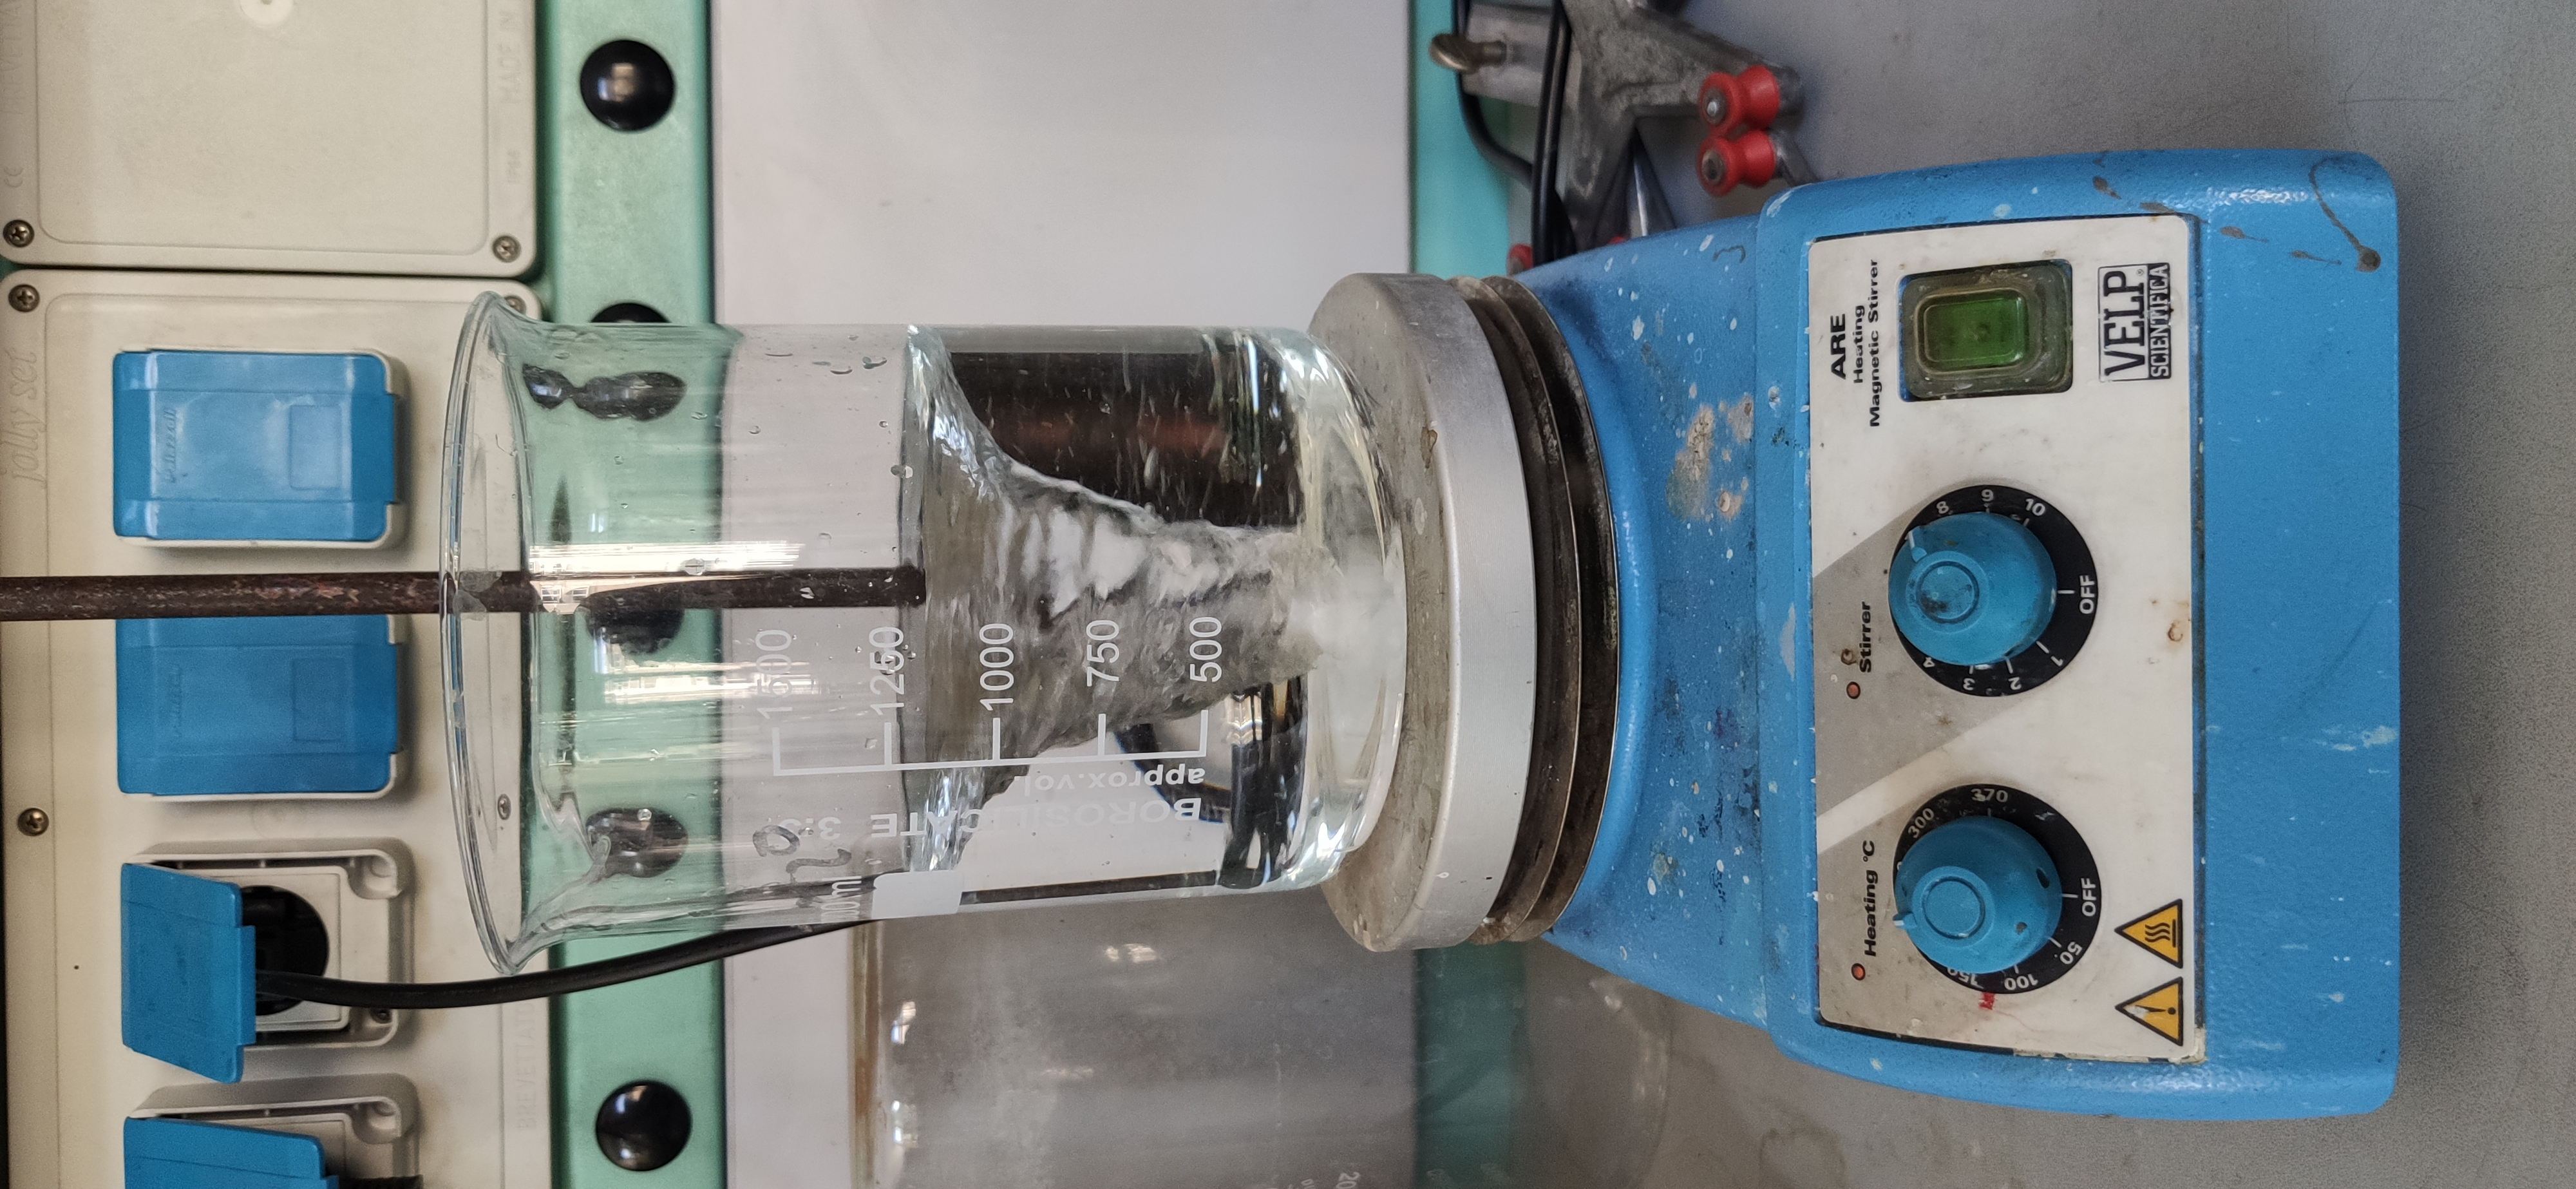
\includegraphics[width=0.5\textwidth]{Pictures/pva_preparation.eps}
                    \caption{A bulk preparation of PVA solution.}
                    \label{fig:PVA}
                \end{figure}

        The initial approach was utilizing mass units only, however PVA can be hard to dissolve in water at room temperature. 
        
        Different batches were prepared by gradually increasing the operational temperature, regulated by a magnetic stirrer-heater. 

        Unless water temperature was kept substantially high (above $70 \ ^{\circ}C $ but still lower than boiling point), 
        solid PVA flakes remained undissolved, despite being stirred for hours. 

        Regardless, defective batches were used during the early experiments, but the undissolved PVA 
        seemed to create a slimy solution that, over time, would produce a thick foam, that potentially clogged 
        the fritted glass filters. 

        Temperatures have been kept higher since then, resulting in no filtering issues down the pipeline. \\ 

        However, despite being able to fully dissolve the solute, water evaporated consistently, making it necessary to refill the 
        container with distilled water, until 1 l of total solution was reached. 

        This was clearly an approximation, compared to the initial choice of utilizing mass measurements only, however 
        the error of a volume filling approach can be considered negligible, given that the 
        percentage of PVA is only $1 \ \%$ by weight and the solution needs to be further diluted down to $0.25 \ \%$ for 
        the precipitation reaction. \\ 

        Dilution to the required fraction of mass is simply obtained by using 100 ml of $1 \ \%$ solution, 
        plus 300 ml of water, for a total of 400 ml. \\ 

        The precipitation reaction is left stirring for 7.5 hours under a 
        chemical hood, starting from the very first drop of PHBH-chloroform solution. 

        This time frame is extremely conservative, as it is very likely that all the residual chloroform is entirely 
        evaporated in a much shorter time, however this aspect has not been tested yet. \\

        At the end of the waiting time, the solution can be filtered with a fritted glass filter, aided by a vacuum 
        ejector. 

        After the PVA solution is filtered out, the remaining powder bed should be washed with isopropyl alcohol and 
        distilled water. 

        Paper filters can be utilized, but the filtering phase would last exponentially longer. Furthermore, the vacuum filtering 
        approach can get rid of almost all of the residual moisture. \\ 

        The obtained powder bed needs to be dried in an oven or a dehydrator, at $40 \ ^{\circ}C$, for at least 12 hours. \\ 

        At this point, the powder should be completely dry and ready to be sieved. \\ 

        A $100 \ \mu m$ sieve has been used, however, smaller size sieves could be used, as many reviews recommend a particle 
        size of $20 \div 80 \ \mu m$ for SLS (as pointed out in section \ref{SLS_general}) \autocites{Padovano_SLS_Review}. 
        
        Powders should be gently pushed against the mesh, alternating with circular motion and shaking of the sieve, should 
        an automated sieving system be unavailable. 

        Several passages might be needed in order to collect most of the powder. \\ 

        Sieved powders should be immediately stored in test tubes or any other sealable container, as they are extremely hygroscopic. 

        With very fine powders, electrostatic interactions with tools and materials should be taken into account, when transferring 
        them into containers. 

        Some losses are expected during this phase, unless specific tools for collecting very fine powders are available. 

        Choosing appropriate materials and reducing material transfer to the minimum amount is essential to minimize 
        powder losses. 

        All tools and containers should be perfectly dry too. 



        \subsection{Initial results and potential issues\label{initial_failures}}

        As mentioned in previous chapters, many failed attempts led to a deeper understanding of the entire process 
        and the proper choice of equipment, tools and tweaking of the initial recipe. \\ 

        The most prominent issue was figuring out the importance of the environmental variables. With higher temperatures, the initially planned amount of chloroform evaporated too 
        quickly while PHBH pellets were being dissolved. 

        The obtained liquid was extremely viscous and hard to drip effectively into the PVA solution. Drippers were constantly clogged
        and, as a result, flow control was unpredictable. 
        
        A thick plastic film covered the internal walls of the drippers and the beakers where PHBH had been dissolved, which 
        introduced the very first significant material waste point in the pipeline. 

        %Moreover, despite being impossible to avoid in general, the excessive thickness of this film that formed in the first batches 
        %severely hindered the cleaning and maintenance of the utilized glassware, which occasionally needed to be cleaned with chloroform 
        %or other solvents. \\ 

        Despite being able to save most initial batches, the final yield was initially insignificant, going as low as 0.1 g of powder 
        per 4 g of raw material. \\ 
        
        %Another factor that severely reduced production rate was the frequent clogging of fritted glass filters. 
        %
        %The undissolved PVA flakes in the first defective batches \ref{detailed_reaction} created a dense foam, which either obstructed 
        %the pores of the filter or slowed the filtration time by orders of magnitude. 
%
        %The clogged filters required to be regenerated with chloroform and rinsed with isopropyl alcohol, in order to regain full 
        %functionality. 

        %In addition to this, some of the filters initially used had already been exploited by other research teams, operating 
        %with metal fines and other materials, which might have contributed to some of the impurities and alien particles detected 
        %by SEM analysis in the earliest samples (\ref{SEM_analysis}). \\ 




    \clearpage

    \section{Recipe tweaking and improvements\label{recipe_improvement}}

    All of the aforementioned attempts (as seen in section \ref{initial_failures}) led to an optimization process that originally aimed at 
    matching the $30 \ \%$ yield obtained by previous researchers, but later far exceeded the 
    initial expectations, improving upon the available blueprint procedure by a wide margin. 


        \subsection{Key variables\label{key_variables}}

        Dealing with a simple yet unstable process, based on theoretical studies and very rough experimental data, requires a
        long trial and error approach, that should carefully isolate each variable, whether it is intrinsic to the 
        involved physical and chemical reactions, environmental, equipment related, or introduced by human 
        interaction with the process. \\ 

        Generally speaking, once all the independent variables are isolated and understood, only a few are extremely relevant and can 
        radically influence the success rate of the entire process. 

        Should these variables be changed, even unintentionally and by a small amount, the final yield
        could be dramatically cut down. \\ 

        It has been pointed out several times that the external temperature is one of the most 
        (if not the absolute most) influential parameter of the entire process, given the fast evaporation pace of chloroform, 
        or organic solvents in general, should the reaction be re-engineered with a less impactful solvent, like the moderate 
        solvents often mentioned in the scientific literature (as mentioned in chapter \ref{Chemical precipitation}) \autocites{Padovano_SLS_Review}.  

        For all the issues discussed in previous chapters, an increase in external temperature correlates with an increase in 
        chloroform use. Starting from the initial 55 ml per 4 g of PHBH pellets, extra chloroform has been added 
        by 2.5 ml increments, until the process stabilized and yield reached a peak that would not benefit from further 
        increase. 
 
        The maximum useful amount of chloroform (per 4 g of PHBH pellets) would be around $65 \div 70 \ ml$. 

        This range consistently produced the highest yield (as discussed in \ref{promising_results}) and not only did further chloroform use stall the 
        results, but it proved to be detrimental over a certain threshold ($ > \ 75 \ ml$), as insufficient 
        viscosity would prevent an accurate flow control during the dripping phase. \\ 

        All these adjustments in chloroform quantity are directly correlated with operational temperatures. A 10 ml 
        increase in chloroform use might seem insignificant at a lab scale, but this would translate to significant waste, 
        should the process be scaled to an industrial level, assuming that no solvent retrieval system is available. 

        %This consideration ties with the environmental sustainability issue \ref{Environmental_impact}, since organic solvents are 
        %inherently impactful and unnecessary waste should not be promoted, especially when sustainable bio-based polymers such as PHBH are involved. 

        Overall, the key parameter that actually matters is viscosity: very low temperatures can minimize chloroform evaporation, 
        but directly increase density and thus viscosity; on the other hand, liquids at higher temperatures should be inherently 
        less viscous, but the drastic solvent evaporation dramatically increases viscosity, simply by having more PHBH and less 
        liquid proportionally. \\ 
        
        The process should be tailored to obtain a PHBH-chlofororm solution with the ideal viscosity, that allows a perfect dripping 
        phase, while producing the highest pellet-to-powder yield. 

        %However, future experiments should focus on achieving this goal with the lowest amount of chloroform possible, which requires 
        %being able to control operational temperature. \\ 

        By contrast, other variables like dripping flow (as previously discussed a drop by drop fashion is ideal but occasional 
        flow distruptions do not seem to have a great influence \ref{detailed_reaction}), or a very precise measure in 
        PVA concentration are not as important for the success of the precipitation process. 

        With a PVA concentration as low as $0.25 \ \%$ and successful reactions even with defective
        solution batches, it is plausible that the precipitation process could be accomplished by 
        substituting PVA with other alcohols such as isopropanol or ethanol or even by simply using distilled water \footnotemark.
        
            \footnotetext{These substitutions could potentially simplify the pipeline, but no experiments have been conducted yet} 

        Assuming the adjustment of viscosity and the optimization of the dripping phase have been dealt with, 
        another relevant parameter is the stirring speed of the PVA solution (see figure \ref{fig:process_diagram} for reference). 

        The experiments conducted during this case study confirm what has been found in the scientific literature: 
        an increase in stirring speed directly correlates to a decrease in average powder particle size, as reminded by figure \ref{fig:stirring_rpm}. 

        However, this correlation is generally measured in terms of RPM, which is an active control of any magnetic stirrer and 
        a good indication of the average rotational speed of the stirred fluid, assuming that the device is properly functioning
        and every other variable is fixed. 
        
        In fact, the RPM controlled by the machine does correlate with the average angular velocity, but does not indicate 
        an exact speed value. 

        For any fixed fluids, should other factors like container size and shape, stirring rod weight and size change, 
        then the average angular velocity would change as well, despite the stirrer being at a fixed RPM value. 

        Since the production rate had been doubled to 8 g of pellets per batch, the reaction has been split into two 
        4 g batches, for lack of single batch capable equipment. 

        Despite perfectly measuring all the quantities and mirroring equipment use for both batches, the magnetic stirrers'
        reported RPM did not match the uneven velocities (even though the utilized models were exactly the same). 

        This aspect is later discussed in further detail \ref{faulty_equipment}. \\ 

        Once this issue has been partially solved with some workarounds, increasing RPM has proven to be an effective 
        strategy to increase final yield: powders were effectively produced at the initially planned 700 RPM, however 
        most of the powder batch could not be sieved under $100 \ \mu m$. 

        Higher RPM values (900 $\div $ 1000 RPM) consistently produced almost no waste during the sieving phase. 


        \subsection{Adaptations and progressively refined equipment choice\label{faulty_equipment}}

        Some of the available equipment was not perfectly suited for the necessary tasks or, sometimes, even broken or malfunctioning. \\ 

        For instance, the drippers used for the precipitation reaction had a manual flow valve, which made flow control unpredictable 
        and hard to regulate. \\ 

        The fritted filters initially used had already been utilized for other production pipelines, transferring some impurities
        to the first samples. This issue was addressed by utilizing a new batch of filters, solely dedicated to the PHBH pipeline. 

        A major issue was the malfunctioning of one of the magnetic stirrers. This caused a few batches to be lost, since the prolonged absence of 
        a stirring motion did not allow for the precipitation process to occur. 

        The defective stirrer was replaced, however, a huge discrepancy 
        in stirring speeds was noticeable, as briefly mentioned in chapter \ref{key_variables}. 

        In spite of the fact that both solutions were prepared identically and the beakers and stirring rods used 
        were exactly the same, one of the stirrers would visibly show a much lower speed at the same RPM value. 

        As an initial workaround, a satisfying speed (based on previous results in terms of final yield) was set on the slower stirrer, 
        then the much faster stirrer was set at a "lower" RPM value, that would visually match the same angular 
        velocity as the reference. \\ 

        This issue was addressed by utilizing two identical stirrers from the same manufacturer, which were set at the same RPM value. \\ 

        Adaptations were needed for storing the sieved powders. With average particle sizes under $ \ 100 \ \mu m$, 
        electrostatic interaction and powder volatility proved to be challenging when handling the final product. 
        
        Sieved powders have been transferred to test tubes or other comparable containers by using folded parchment paper. \\ 

        
        All the workarounds and adaptations can normally be part of a very experimental lab workflow, but the process should ideally 
        be capable of producing even greater yields, once it is scaled for industrial production, where each step is standardized 
        and custom equipment tailored to specific tasks. 

        \clearpage

        \subsection{Current results in the powder production pipeline \label{promising_results}}

        Compared to the earliest batches, even the experiments conducted by previous researchers held substantially better 
        results, with maximum yields of $30 \ \%$. \\ 

        The minimum requirement for the current case study was that of replicating the previous records but, after 
        a huge amount of failed attempts, optimization and tweaking in the entire process pipeline, current results 
        far exceed the initial expectations, with even more room for improvement. \\ 

        The pellet-to-powder yield has increased to a minimum of 5 g of powder and a maximum of 6 g, over 8 g of raw material. 

        The current yield ranges between $62.5 \ \%$ and $75 \ \%$, which is a relative improvement of $2 \div 2.5$ times that 
        achieved in the previous research that this work is based on, and over an order of magnitude increase compared to the 
        initial experiments. \\ 
%
%        \begin{figure}[h]
%            \centering
%            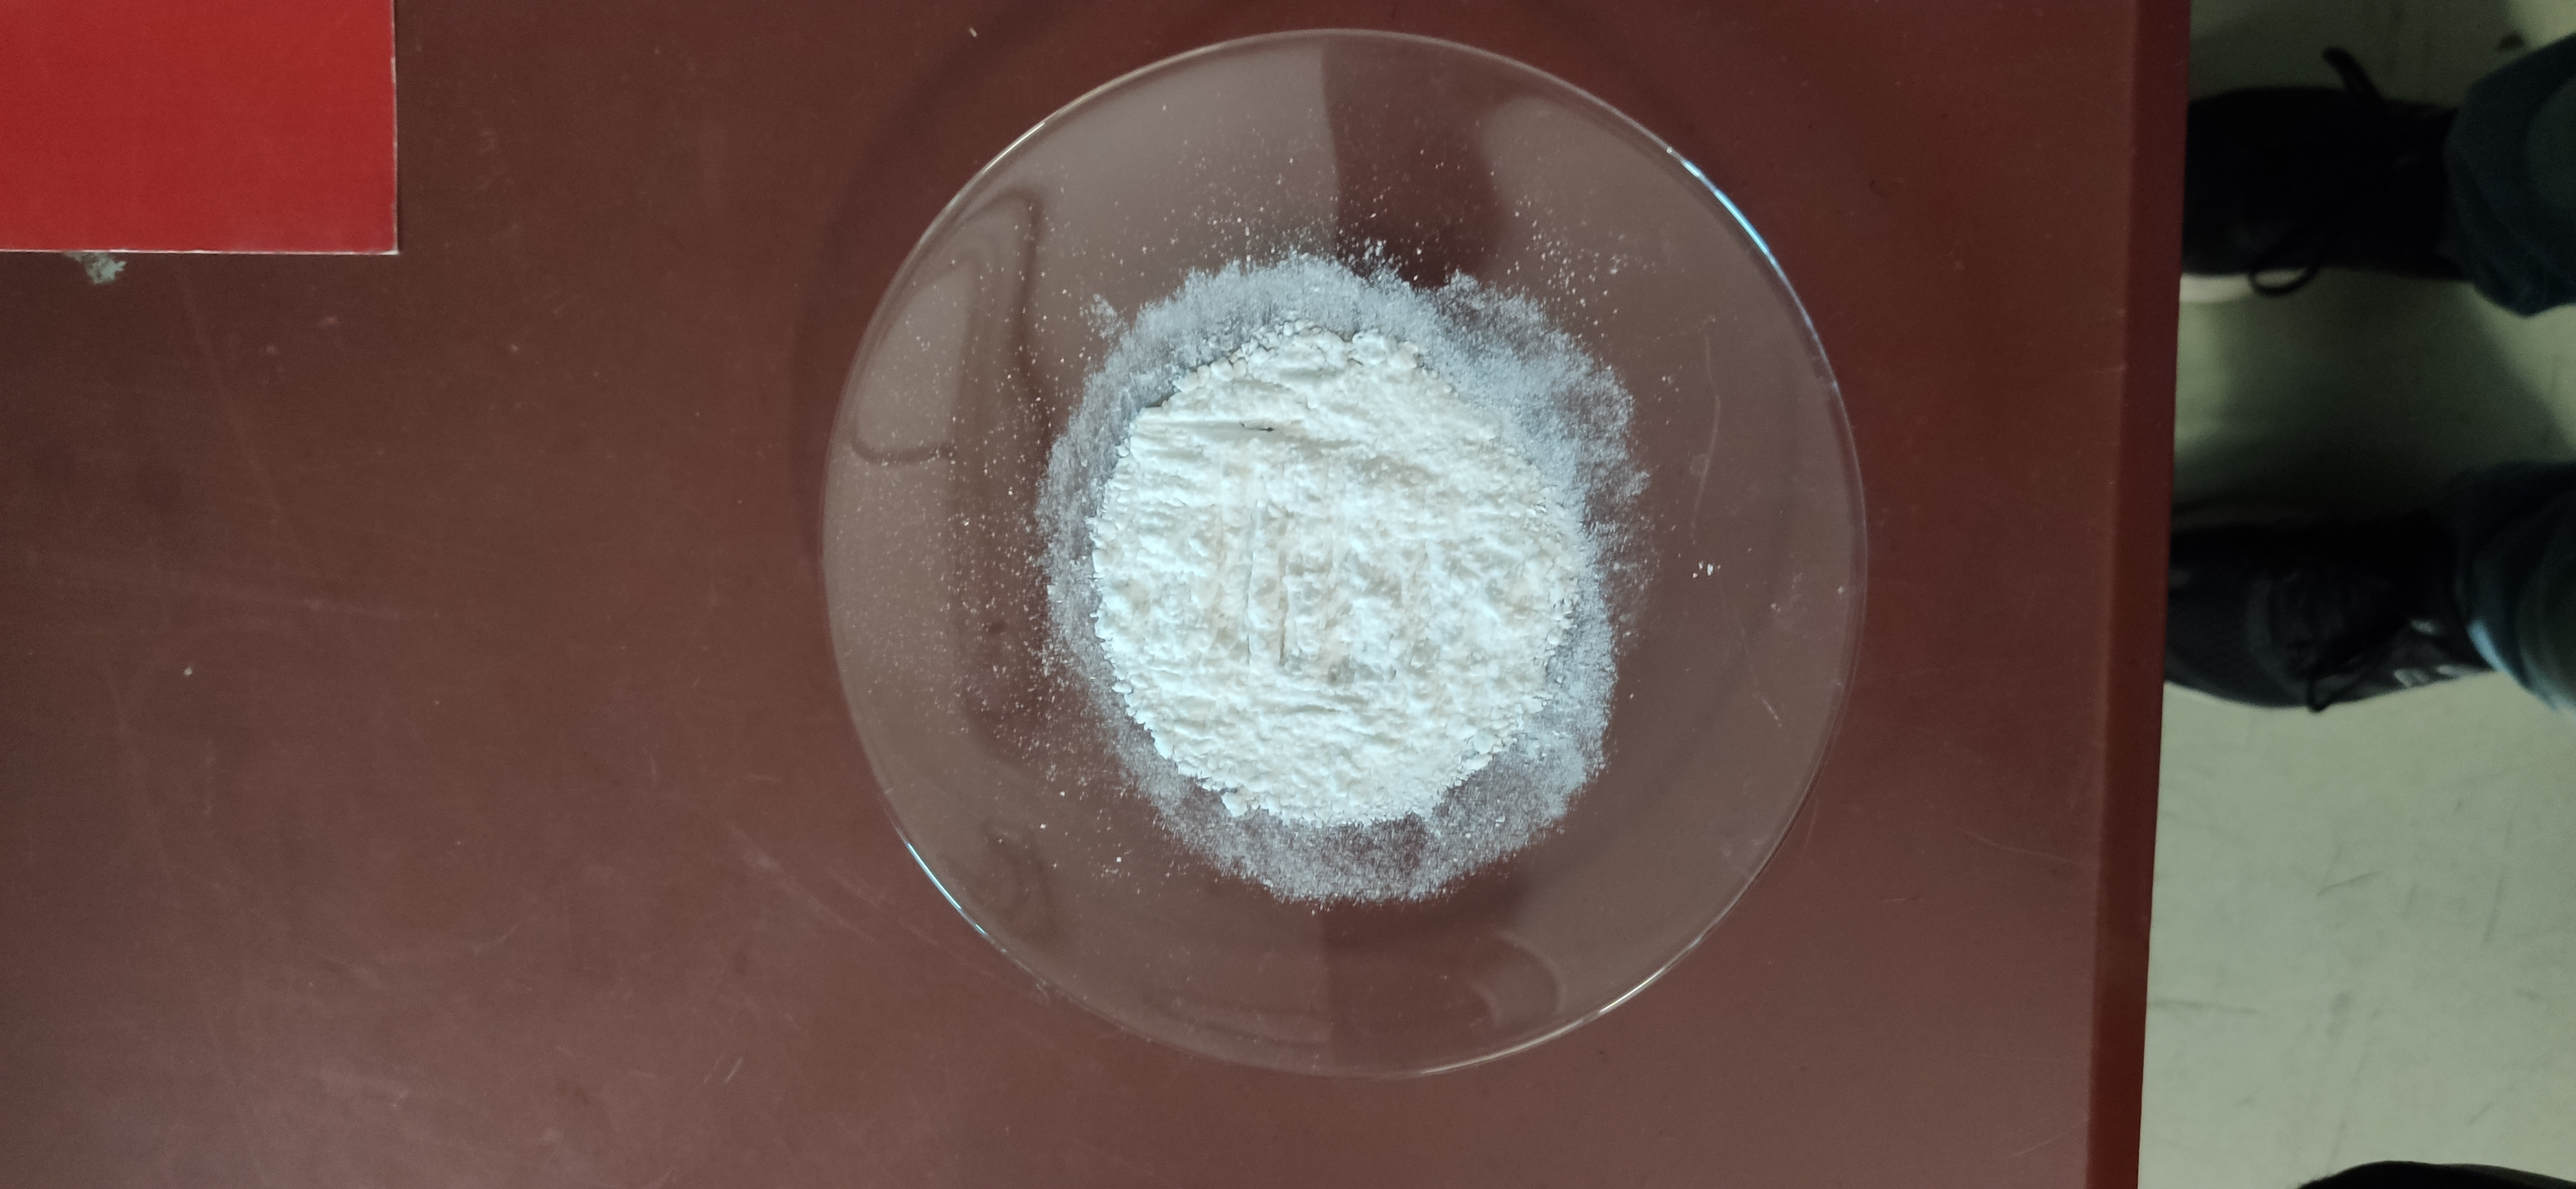
\includegraphics[width=0.5\textwidth]{Pictures/PHBH_dried_powder.eps}
%            \caption{Dried powder batch obtained from the current production pipeline.}
%            \label{fig:dried_powder}
%        \end{figure}
%

        \subsubsection{Consistent reproducibility and scalability\label{consistent_reproducibility}}

        Not only has the total yield been improved, but the process has been stabilized and better understood in all of its 
        peculiarities, as already explained in chapter \ref{key_variables}. 

        Until all the optimization work had been accomplished, the process held inconsistent results, with powder quantities drastically 
        varying from insignificant to mediocre yields. \\ 

        A key aspect of a reliable process is in fact its consistent reproducibility under known and controllable conditions, 
        which is necessary (but not sufficient) for large scale production and adoption at industrial scale. \\ 

        The latest results have been reproduced consistently in the lab and might be scaled to higher production rates after 
        further optimization. \\ 




    \clearpage
    \section{Powder granulometry and morphology\label{powder_granulometry_morphology}} 

    While obtaining some form of powder with the precipitation process was somewhat expected, all the work would be 
    pointless if the criteria discussed at the beginning of this research were not met, as highlighted in \ref{Powder_requirements}. \\ 

    The powders produced would not be suitable for SLS additive manufacturing, if granulometry (average grain size distribution)
    were not under a certain size threshold and if the morphology of those powders were not close to a non hollow spherical geometry 
    \autocites{Padovano_SLS_Review}. \\

    While an adequate maximum size threshold is guaranteed by sieving the powders,
    investigations in terms of particle size distribution (as showcased in detail in chapter \ref{granulometry_analysis})
    are needed in order to evaluate the overall granulometry. 
    
    In addition to this, adequate morphology can only be 
    determined by visual inspection of SEM (\textit{Scanning Electron Microscopy}) images, as explained in chapter \ref{SEM_analysis}. \\

    Sieving is an essential step when selecting SLS suitable powders. \\ 
    A general guideline on SLS powders granulometry is that particles should be smaller than $100 \ \mu m$, with many 
    sources in the literature reporting an ideal range of $20 \div 80 \ \mu m$ \autocites{Padovano_SLS_Review}. \\ 

    The powders obtained during the very first experiments produced a lot of waste during the sieving phase, which was due to their excessive size. 

    However, with the currently optimized process, the powder batches produced little to no waste during sieving, which has been achieved 
    with a $100 \ \mu m$ sieve. \\

    \clearpage

    \section{Powder and 3D printed parts characterization\label{powder_characterization}}

    The powder produced by the precipitation process has been characterized in terms of granulometry, morphology, gas pycnometry and flowability, 
    as well as thermal properties, as later discussed in detail in chapters \ref{Thermal_analysis}, \ref{density_measurement}, 
    \ref{flowability_analysis}, \ref{granulometry_analysis} . \\

    As all the mentioned analyses highlighted excellent results, well within the desired SLS requirements seen in section \ref{Powder_requirements}, the powder has been successfully used to produce 3D printed parts
    (showcased in chapter \ref{SLS_printing_experimental}), which have been characterized in terms of mechanical properties, as well as thermal properties, that have been 
    compared to those of the powder and the original raw material. \\

    Overall, all of the analyses have shown that the PHBH powder produced by the precipitation process is suitable for SLS additive manufacturing, which is in itself a huge achievement for a 
    novel and experimental process, given the fact that the powder is produced from a bio-based polymer that is not commonly used in the additive manufacturing industry, and that 
    the available literature on the subject has highlighted the difficulty of obtaining SLS suitable powders from biopolymers \autocites{Padovano_SLS_Review}. \\ 

    Moreover, in addition to producing an SLS suitable powder, with an excellent yield, the 3D printing process has been successful as well, with 
    a lot more potential to be explored in the future. \\ 

    As a final note, one of the main goal of the carried out analyses was to address the potential change in thermal properties of the biopolymer, during the entire pipeline. 
    
    As shown in detail in the following chapters, both the powder and the printed parts have shown no significant thermal properties changes, compared to the 
    original raw material, which is an extremely important aspect, given how bio-based materials are tipycally more sensitive to thermal degradation. \\ 


    \clearpage
        \subsection{SEM (Scanning Electron Microscopy) analysis\label{SEM_analysis}}

        Scanning Electron Microscopes are widely used detection instruments, which unlike traditional microscopes 
        do not utilize optical lenses, but reconstruct images generated by the interaction between an electron beam and the targeted 
        sample. \\ 

        There are several inspection techniques that could be exploited using different SEMs, however the most suitable for inspecting 
        fine powder morphology is the image reconstruction through SE (\textit{Secondary Electrons}) emission. 

        When invested by a high energy electron beam, the inelastic interaction with secondary low energy electrons ($< 50 \ eV$) triggers their emission from the valence bands of the specimen atoms and scatters them. 

        The emission of secondary electrons happens within a few nm inside the specimen, which makes this method perfectly suited 
        for highlighting particle overall shape and surface displacement, to a high degree of detail and precision. \\

        SEM images have been produced with multiple specimens, on samples collected during the entire duration of the experimental 
        activities, which is later discussed in detail in section \ref{SEM_analysis_results}. 

        The expected particle morphology should ideally approach that of perfect non hollow sphere, as pictured in figure \ref{fig:SEM_DALLE2}, generated by \textit{Dall-E 2}'s 
        text prompt-to-image artificial intelligence algorithm \autocites{DALLE2}{DALLE2_roundparticles}. 

            \begin{figure}[h!]
                \centering
                \includegraphics[width=0.7\textwidth]{Pictures/SEM/Edited/DALL·E 2022-08-18 16.33.26 - Round particles seen through a SEM microscope.png}
                \caption{Prompt: \textit{"Round particles seen through a SEM microscope"}}
                \label{fig:SEM_DALLE2}
            \end{figure}

            \clearpage

            As mentioned, samples have been collected throughout the entirety of the experimental activity, which has been characterized by a lot of trial and error, 
            before the entire production pipeline got optimized and 
            under perfect control. \\ 

            The experiment has been conducted using a \textit{FIB-SEM, TESCAN S9000G, Tescan} instrument, which is a high resolution 
            scanning electron microscope, equipped with a focused ion beam (FIB) for sample preparation and 
            an electron backscatter diffraction (EBSD) detector \autocites{FIB-SEM_TESCAN_S9000G}. \\

            The collected specimens have been selected, categorized and then assigned an ID:

            \begin{equation}
                ID = SEM_{NN}
                \label{eq:SEM_ID}
            \end{equation}

            where $SEM_{NN}$ is the sample's absolute ascending time number. \\ 


            All the selected samples have been catalogued as follows:

            \begin{table}[h!]
                \centering
                \resizebox{0.4\textwidth}{!}{%
                    \begin{tabular}{@{}ccccccc@{}}
                        \toprule
                        \textbf{ID}               & Magnification  \\ \midrule
                        \textbf{$SEM_{01}$}       & 461 X          \\
                        \textbf{$SEM_{02}$}       & 461 X          \\
                        \textbf{$SEM_{03}$}       & 461 X          \\
                        \textbf{$SEM_{04}$}       & 461 X          \\
                        \textbf{$SEM_{05}$}       & 461 X          \\
                        \textbf{$SEM_{06}$}       & 461 X          \\
                        \textbf{$SEM_{07}$}       & 800 X          \\
                        \textbf{$SEM_{08}$}       & 800 X          \\
                        \textbf{$SEM_{09}$}       & 800 X          \\
                        \textbf{$SEM_{10}$}       & 400 X          \\
                        \textbf{$SEM_{11}$}       & 400 X          \\
                        \textbf{$SEM_{12}$}       & 400 X          \\ \bottomrule
                    \end{tabular}%
                }
                \caption{All catalogued SEM samples}
                \label{tab:SEM_samples_catalogue}
            \end{table}

            The samples have been collected in a total of 12 different occasions, with a total of 12 different specimens. \\


            The main instrument parameters to be modified during the experiment were the electron beam energy, the working distance, the magnification 
            factor and the signal type.  \\
            The electron beam energy has been set to 10 kV for the first 6 samples, using the secondary electrons signal at constant pressure (SE)
            and then to 20 kV for the remaining 6 samples, using the variable pressure secondary electrons signal (VPSE G4). \\

            Different magnifications factors have been used, ranging from 400 to 800 X, to showcase different particle sizes and to better understand 
            the particle morphology. \\

            All SEM images have been AI upscaled and enhanced with basic raster image editing workflows. \\ 

                \begin{figure}[h!]
                    \centering
                    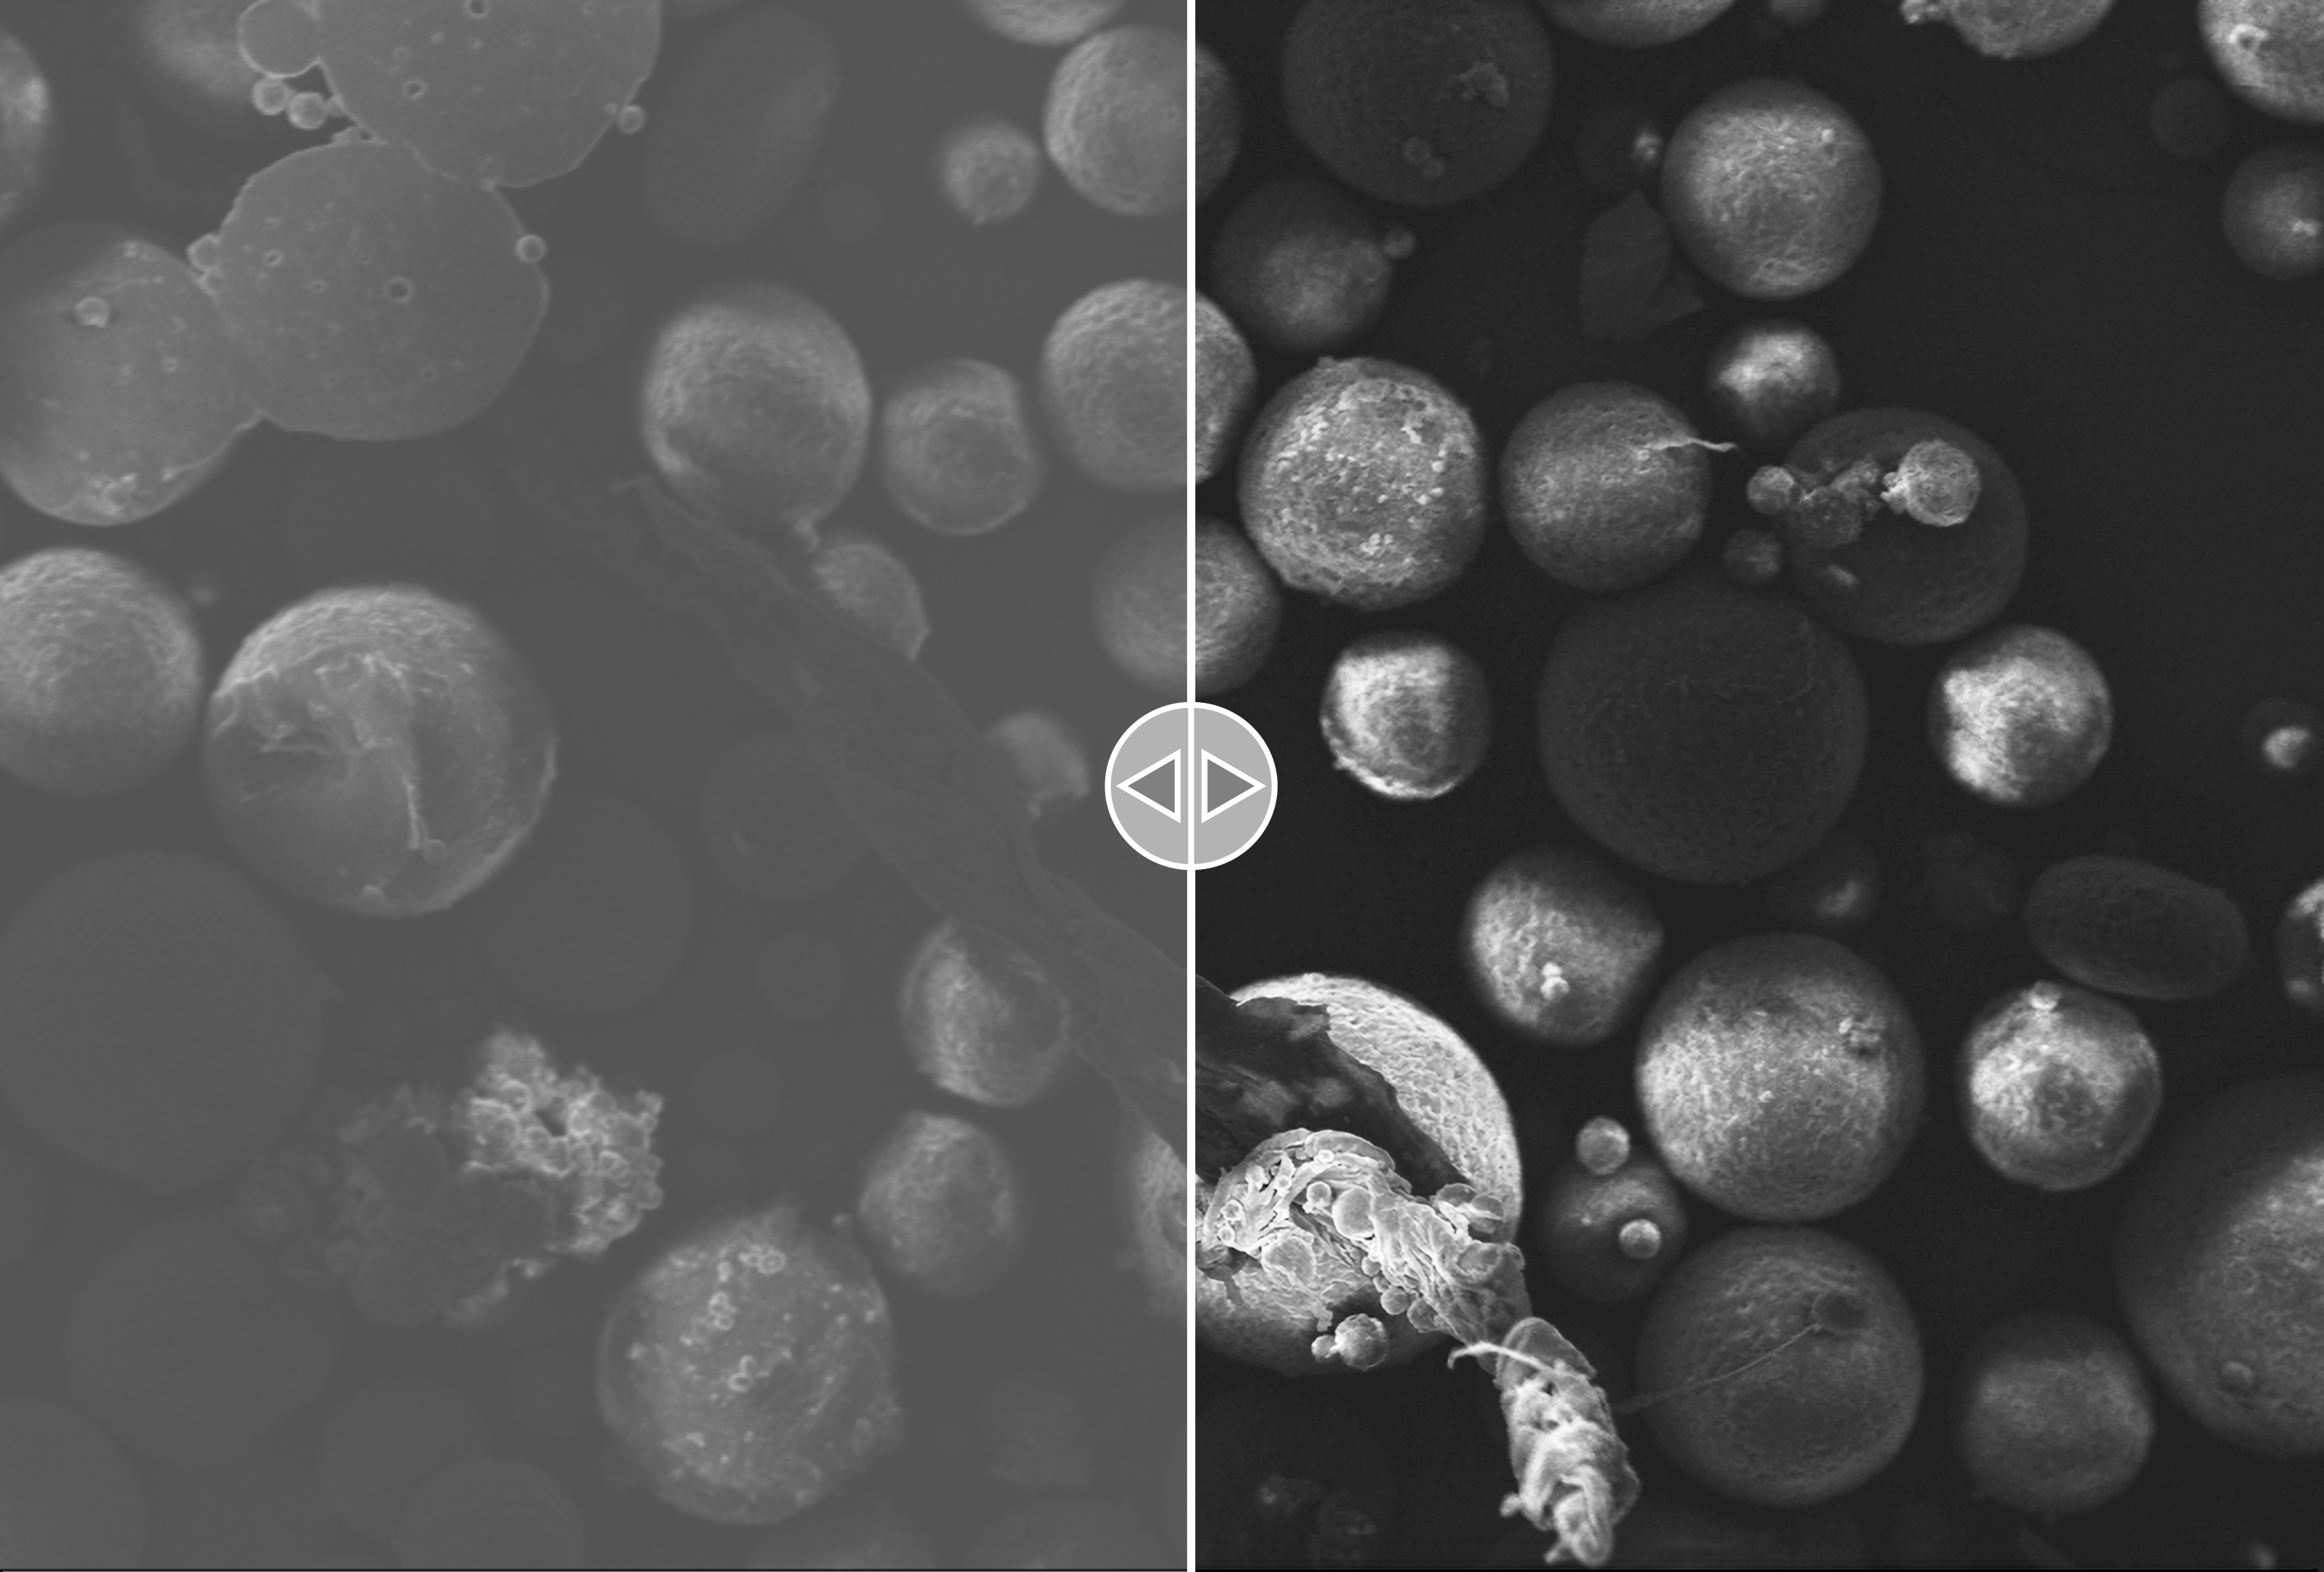
\includegraphics[width=\textwidth]{Pictures/SEM/Edited/unedited_vs_edited.png}
                    \caption{Example of a SEM image before and after enhancing \autocites{Inkscape}{Pixelmator_Pro}}
                    \label{fig:SEM_edited_vs_unedited}
                \end{figure}

            \clearpage

            \subsection{Thermal analysis\label{Thermal_analysis}}
    
            Various thermal analysis tools have been utilized in this thesis work, as many critical properties of the studied material 
            can be deducted with different measurments at various temperature ranges. 

            This is especially true with materials suited for SLS, where knowledge of thermal properties is 
            essential in determining a polymer's feasibility for this AM method. 
            The thermal analysis tools used in this case study are the DSC (\textit{Differential Scanning Calorimetry}) and the TGA
            (\textit{Thermogravimetric Analysis}). \\

            \subsubsection{DSC (Differential Scanning Calorimetry)\label{DSC_analysis}}
        
            \textit{Differential Scanning Calorimetry} is a thermoanalytical technique that can be implemented with different types of machines, 
            but its general purpose is the analysis of the change in heat flow as a function of temperature, which is generally increased in 
            a linear fashion. 
        
            
            The term differential in DSC indicates that each test sample is analyzed in parallel to a reference sample, whose heat capacity and 
            thermal properties are well known and used to calibrate the machine. \\
            
            A typical use of DSC is the detection of phase transitions, which is crucial for applications such as SLS, where each material 
            needs to be locally fused within an optimal sintering window \ref{Powder_requirements}, \ref{PHBH}. 
    
            One of the greatest advantage of PHBH over comparable materials is its wider sintering window, which makes it ideal 
            for SLS \ref{PHBH}. \\ 
    
            This sintering window can be measured by analyzing a DSC plot of heat flow over temperature, given that this test measures 
            phase transitions but is also capable of detecting more subtle physical changes, such as glass transition. 
    
            Since the sintering window is defined as the temperature range comprised between cold crystallization offset and 
            melting point onset \ref{Powder_requirements}, both detected by a DSC analysis \ref{fig:DSC_10Cmin}, then calculating it is trivial, 
            based on the available data.

                The DSC machine used in this thesis work is the \textit{DSC 214 Polyma Equipment} \autocites{Netzsch}, which is a benchtop instrument that can be used for 
                a wide range of applications, shown in figure \ref{fig:DSC_polyma}. \\ 

                It is equipped with a gas controller and has been used in the temperature range from $-50 \ ^{\circ} C$ 
                to $180 \ ^{\circ} C$ with 
                a heating rate of $10 \ (or \ 5) \ °C/min$, and from $180°$ to $-50 \ °C$ with a cooling rate of $10  \ ^{\circ}C/min$, 
                under nitrogen flow $(50 \ mL/min)$. \\ 

                The included software allows for the analysis of the 
                DSC data, as well as the creation of a report with the results. \\ 

                    \begin{figure}[h!]
                        \centering
                        \includegraphics[width=0.7\textwidth]{Pictures/DSC_Polyma.eps}
                        \caption{DSC 214 Polyma Equipment by Netzsch Group}
                        \label{fig:DSC_polyma}
                    \end{figure}

                Multiple DSC analysis have been conducted and specimens have been catalogued with the following ID: 

                \begin{equation}
                    ID = xDSC_{NN}
                    \label{eq:DSC_ID}
                \end{equation}

                where x is either \textit{g} for granule or \textit{p} for powder, and NN is the sample's absolute 
                ascending time number. \\

                The specimens have been catalogued as follows: 

                \begin{table}[h!]
                    \centering
                    \resizebox{0.8\textwidth}{!}{%
                    \begin{tabular}{@{}cccccc@{}}
                    \toprule
                    \textbf{ID}                 & \textit{Weight {[}mg{]}} & \textit{Temperature ramp {[}°C/min{]}}  \\ \midrule
                    $gDSC_{01}$                 & 8.5000                   & 10.0000                                       \\
                    $pDSC_{02}$                 & 8.0000                   & 10.0000                                        \\
                    \bottomrule
                    \end{tabular}% 
                    }
              \caption{Selected DSC specimens representing a granule and a powder sample}
              \label{tab:DSC_ID}
              \end{table} 

              \clearpage

        \subsubsection{TGA (Thermal Gravimetric Analysis)\label{TGA_Analysis}}
        
        \textit{Thermal Gravimetric Analysis} is a technique that constantly measures the mass of an object subjected to a deliberate 
        change in temperature for a certain period of time, through a precision scale. 

        Time, temperature and mass are the involved variables and while mass is a direct measure, whose sudden changes (visible peaks
        in the weight vs temperature plot) can indicate relevant transition points, time and temperature are directly controlled 
        as machine parameters. \\ 

        Generally speaking, TGA instruments can be set up for different workflows: 

                \begin{itemize}
                    \item static or isothermal analysis, where weight changes are registered over a specified time frame, 
                    at a fixed temperature of interest
                    \item quasi-static analysis, where temperature is changed in discrete steps, with isothermal intervals in between 
                    \item dynamic analysis, where temperature is changed in a continuous linear fashion
                \end{itemize}

            The analysis can be set up to end after a certain time, temperature or residual weight and be performed 
            in vacuum, air or inert gas such as argon. \\

        This analysis technique can be used to reveal many important temperature values where physical transformations or chemical 
        reactions occur, pinpoint the presence of certain materials with known transition points, in samples of unknown composition, 
        (e.g residual moisture can be detected by checking any sudden weight changes around $100 \ ^{\circ}C $, water's boiling point), 
        determine the complete degradation cycle of a sample, testing the thermal stability of a material at its operational temperature, etc. \\ 

        The analysis has been firstly performed on the raw pellet material, as a benchmark test
        that consistently returned the expected degradation behaviour, over multiple analysis. 

            The test has then been conducted on powder samples and SLS printed samples, focusing on finding relevant 
            discrepancies with the reference behaviour, which could potentially highlight the presence of impurities
            that might have been undetected during SEM analysis (\ref{SEM_analysis}). \\ 

            The TGA analysis was performed on a \textit{Mettler-Toledo TGA/SDTA 851e} \autocites{Mettler_Toledo} instrument (seen in figure \ref{fig:TGA_mettlertoledo}), 
            in air atmosphere, with a heating rate of $10 \ ^{\circ}C/min$ and a temperature range of $25 \ ^{\circ}C$ to $900 \ ^{\circ}C$. \\

            \begin{figure}[h!]
                \centering
                \includegraphics[width=0.7\textwidth]{Pictures/TGA_mettlertoledo.eps}
                \caption{Mettler-Toledo TGA/SDTA 851e \autocites{Mettler_Toledo}}
                \label{fig:TGA_mettlertoledo}
            \end{figure}

            The specimens that have undergone a TGA analysis have been assigned an ID with the following criteria:

                \begin{equation}
                    ID = xTGA_{NN}
                    \label{eq:TGA_ID}
                \end{equation}

            where $x$ is the specimen type (granule, powder or sintered), and $NN$ is the sample number. \\

            The specimens have been catalogued in the following table:

                    \begin{table}[h!]
                        \centering
                        \resizebox{0.5\textwidth}{!}{%
                        \begin{tabular}{@{}ccc@{}}
                        \toprule
                        \textbf{ID}  & Type     & Weight {[}mg{]} \\ \midrule
                        $gTGA_{01}$ & pellet    & 29.0641         \\
                        $pTGA_{02}$ & powder    & 15.4821         \\
                        $pTGA_{03}$ & powder    & 38.2253         \\
                        $sTGA_{04}$ & sintered  & 10.5330         \\ \bottomrule
                        \end{tabular}%
                        }
                        \caption{TGA specimens}
                        \label{tab:TGA_specimens}
                    \end{table}

        \clearpage

        \subsection{Density analysis\label{density_measurement}}
        The true density of the powder is an important parameter to determine its flowability, which is a key factor in the
        SLS printing process, as better described in (\ref{flowability_analysis}). \\
        
        Its value should be ideally identical to the theoretical density of the material, which is stated to be 
        $1.20 \ kg/m^3$ in its datasheet \autocites{GruppoMaip}. \\ 
        
        The density of the powder has been measured with a \textit{Ultrapyc 5000 gas
        pycnometer} \autocites{Ultrapyc5000}. \\ 
    
        \begin{figure}[h!]
            \centering
            \includegraphics[width=0.7\textwidth]{Pictures/pycnometer.eps}
            \caption{Ultrapyc 5000 gas pycnometer \autocites{Ultrapyc5000}}
            \label{fig:ultrapyc5000}
        \end{figure}
    
        A 0.626 g sample of the powder has been weighed and placed in the sample cell, then the pycnometer has been filled with 
        helium gas and the measurements have been performed at $20 \ ^{\circ}C$, using the \textit{pulse} preparation and the 
        \textit{fine powder} flow rate presets available in the device settings. \\ 
    
        The test has been iterated with a total of 15 steps, with a $0.01 \%$ precision and three measurements per pass, giving an average 
        density value of $1.213602 \ kg/m^3$, consistent with the expected theoretical value. \\ 
    
        \clearpage

        \subsection{Flowability analysis\label{flowability_analysis}}

        The flowability of a powder is a key factor in the success of the SLS process, as it impacts the way the powder is deposited
        on the build platform. Some powders are more prone to clumping, which can lead to the formation of bridges between the powder 
        particles, which can cause the build platform to become clogged and the build to fail. \\ 

        A powder with a good flowability will be able to flow freely and evenly, without clumping, and will be able to fill the 
        build platform evenly, without leaving any gaps. \\ 

        Powders with poor flowability can be improved by adding a flowability agent, which can be a lubricant, a binder or a 
        combination of both. \\ 

        The flowability of a powder can be tested by performing a flowability analysis, which can be performed in a number of ways, 
        depending on the standard that is being followed. \\

        The analysis has been performed on the powder samples, using the \textit{tap density} method, which is the most common 
        approximation test, as described by ASTM D7481 \autocites{ASTM_D7481-18}. \\

        The standard describes how to evaluate the packing factor and the Hausner Ratio of a powder sample (that needs to be 
        dried, before being tested, as residual moisture negatively impacts the flowability), 
        using a 100 mL graduated cylinder, following the steps described for procedure \textit{b}. \\

        The Hausner Ratio is evaluated with the equation described in previous chapters \ref{eq:Hausner_ratio}, \ref{Powder_requirements}, 
        and the packing factor is evaluated with the following equation: 

            \begin{equation}
                \varphi  = \frac{\rho_{bulk}}{\rho}
                \label{eq:packing_factor}
            \end{equation}

        where $\rho_{bulk}$ is the bulk density and $\rho$ is the true material density. \\

        As previously mentioned in \ref{Powder_requirements} and according to the available literature, the Hausner Ratio of the powder should 
        be ideally below 1.4 \autocites{doi:10.1063/1.4918516}, which is consistent with the experimental findings. \\  

        \clearpage

        \subsection{Granulometry analysis\label{granulometry_analysis}}

        The granulometry analysis has been performed on an oven dried powder sample, 
        using a \textit{Malvern Morphologi 4} \autocites{Malvern_Morphologi4}. \\ 

        \begin{figure}[h!]
            \centering
            \includegraphics[width=0.7\textwidth]{Pictures/malvern.eps}
            \caption{Malvern Morphologi 4 \autocites{Malvern_Morphologi4}}
            \label{fig:morphologi4}
        \end{figure}

        The sample has been measured in terms of volume, with a $5 \ mm^3$ specimen being spread on a glass plate in the 
        most homogeneous way possible, by using a 4 bar dispersion pressure and a 10 ms injection time. \\ 

        An homogenous powder distribution is crucial in order to avoid particle overlap and to obtain a more accurate 
        representation of the powder granulometry. \\ 

        The instrument has taken several images of the powder specimen, using a 10X magnification, and by z-stacking 
        images with different focal lenghts, in order to achieve better results. \\

        All particles below 20 $\mu m$ have been excluded from the analysis, which has been performed by using an automated 
        static imaging algorithm, performed by the instrument's software. \\ 

      \clearpage

      \subsection{Dynamic Mechanical Analysis\label{DMA}}
 
        A non-destructive DMA has been used to determine some of the mechanical properties of SLS printed PHBH. The analysis 
        allows for the determination of the storage modulus $E'$, the loss modulus $E''$ as well as the tan$\delta$, 
        which is the ratio between the loss modulus and the storage modulus. \\ 
        As mentioned in \ref{DSC_analysis}, the DMA can also be used to better determine the glass transition temperature $T_g$, which 
        has been initially estimated to be around $2 \ ^{\circ}C$ by the DSC analysis of a PHBH powder sample, as visible in figure \ref{fig:DSC_10Cmin}. 
        However, the revealed 
        peak activity in that temperature range can not be attributed to the glass transition in a definitive way, by means of a DSC analysis 
        alone. \\ 

        The glass transition temperature, which is defined as the temperature at which the material changes from a glassy to a rubbery state, 
        (i.e. the temperature at which the material changes its stress-strain behavior from brittle to plastic), can be determined with 
        better precision by a DMA. \\ 

        More specifically, the transition point can be revealed by a prominent peak in the tan$\delta$ curve, indicating a 
        sudden change in the moduli ratio of the material. \\ 
        
        The analysis has been performed with a Triton Technology DMA instrument \autocites{Triton_Technology_Ltd}, on the SLS sample 
        $10-DMA01_{filled}$ that has been printed specifically for the purpose of the DMA analysis 
        (as said in sections\ref{SLS_printing_experimental}, \ref{tab:SLS_samples}, \ref{fig:printed_specimens_DMA}). \\ 

        The test has been run with an oscillating uniaxial stress amplitude of 1 N, at a frequency of 1 Hz, with an initial 
        chamber temperature of $- 77.7 \ ^{\circ}C$ (achieved by cooling the environment with liquid nitrogen), and has been stopped 
        once the sample reached the rubbery plateau, i.e. a temperature region below the melting point, in which the material 
        exhibits an almost constant modulus behaviour \autocites{JD_Ferry_viscoelasticpolymers}. \\


      \section{Analyses results\label{analyses_results_general}}

      Given the wide variety of instruments and their vastly different release date, the various included software suites and operating systems involved,
      all the different output files have been analyzed and uniformed as tab separated values UTF-8 text, using standard unix cli tools. \\ 
      
      The uniforming of datasets later favoured the data analysis workflow, which has been performed by using \textit{GNU Octave} \autocites{Octave} and \textit{Labplot} \autocites{Labplot}. \\

      \subsection{SEM Results\label{SEM_analysis_results}}

                
      The FIB-SEM instrument has produced a total of 12 different images, the most relevant have been edited using 
      \textit{Pixelmator Pro} and \textit{GIMP} \autocites{Pixelmator_Pro}{GIMP} and are shown below: \\

          %\begin{figure}[h!]
          %    \centering 
          %    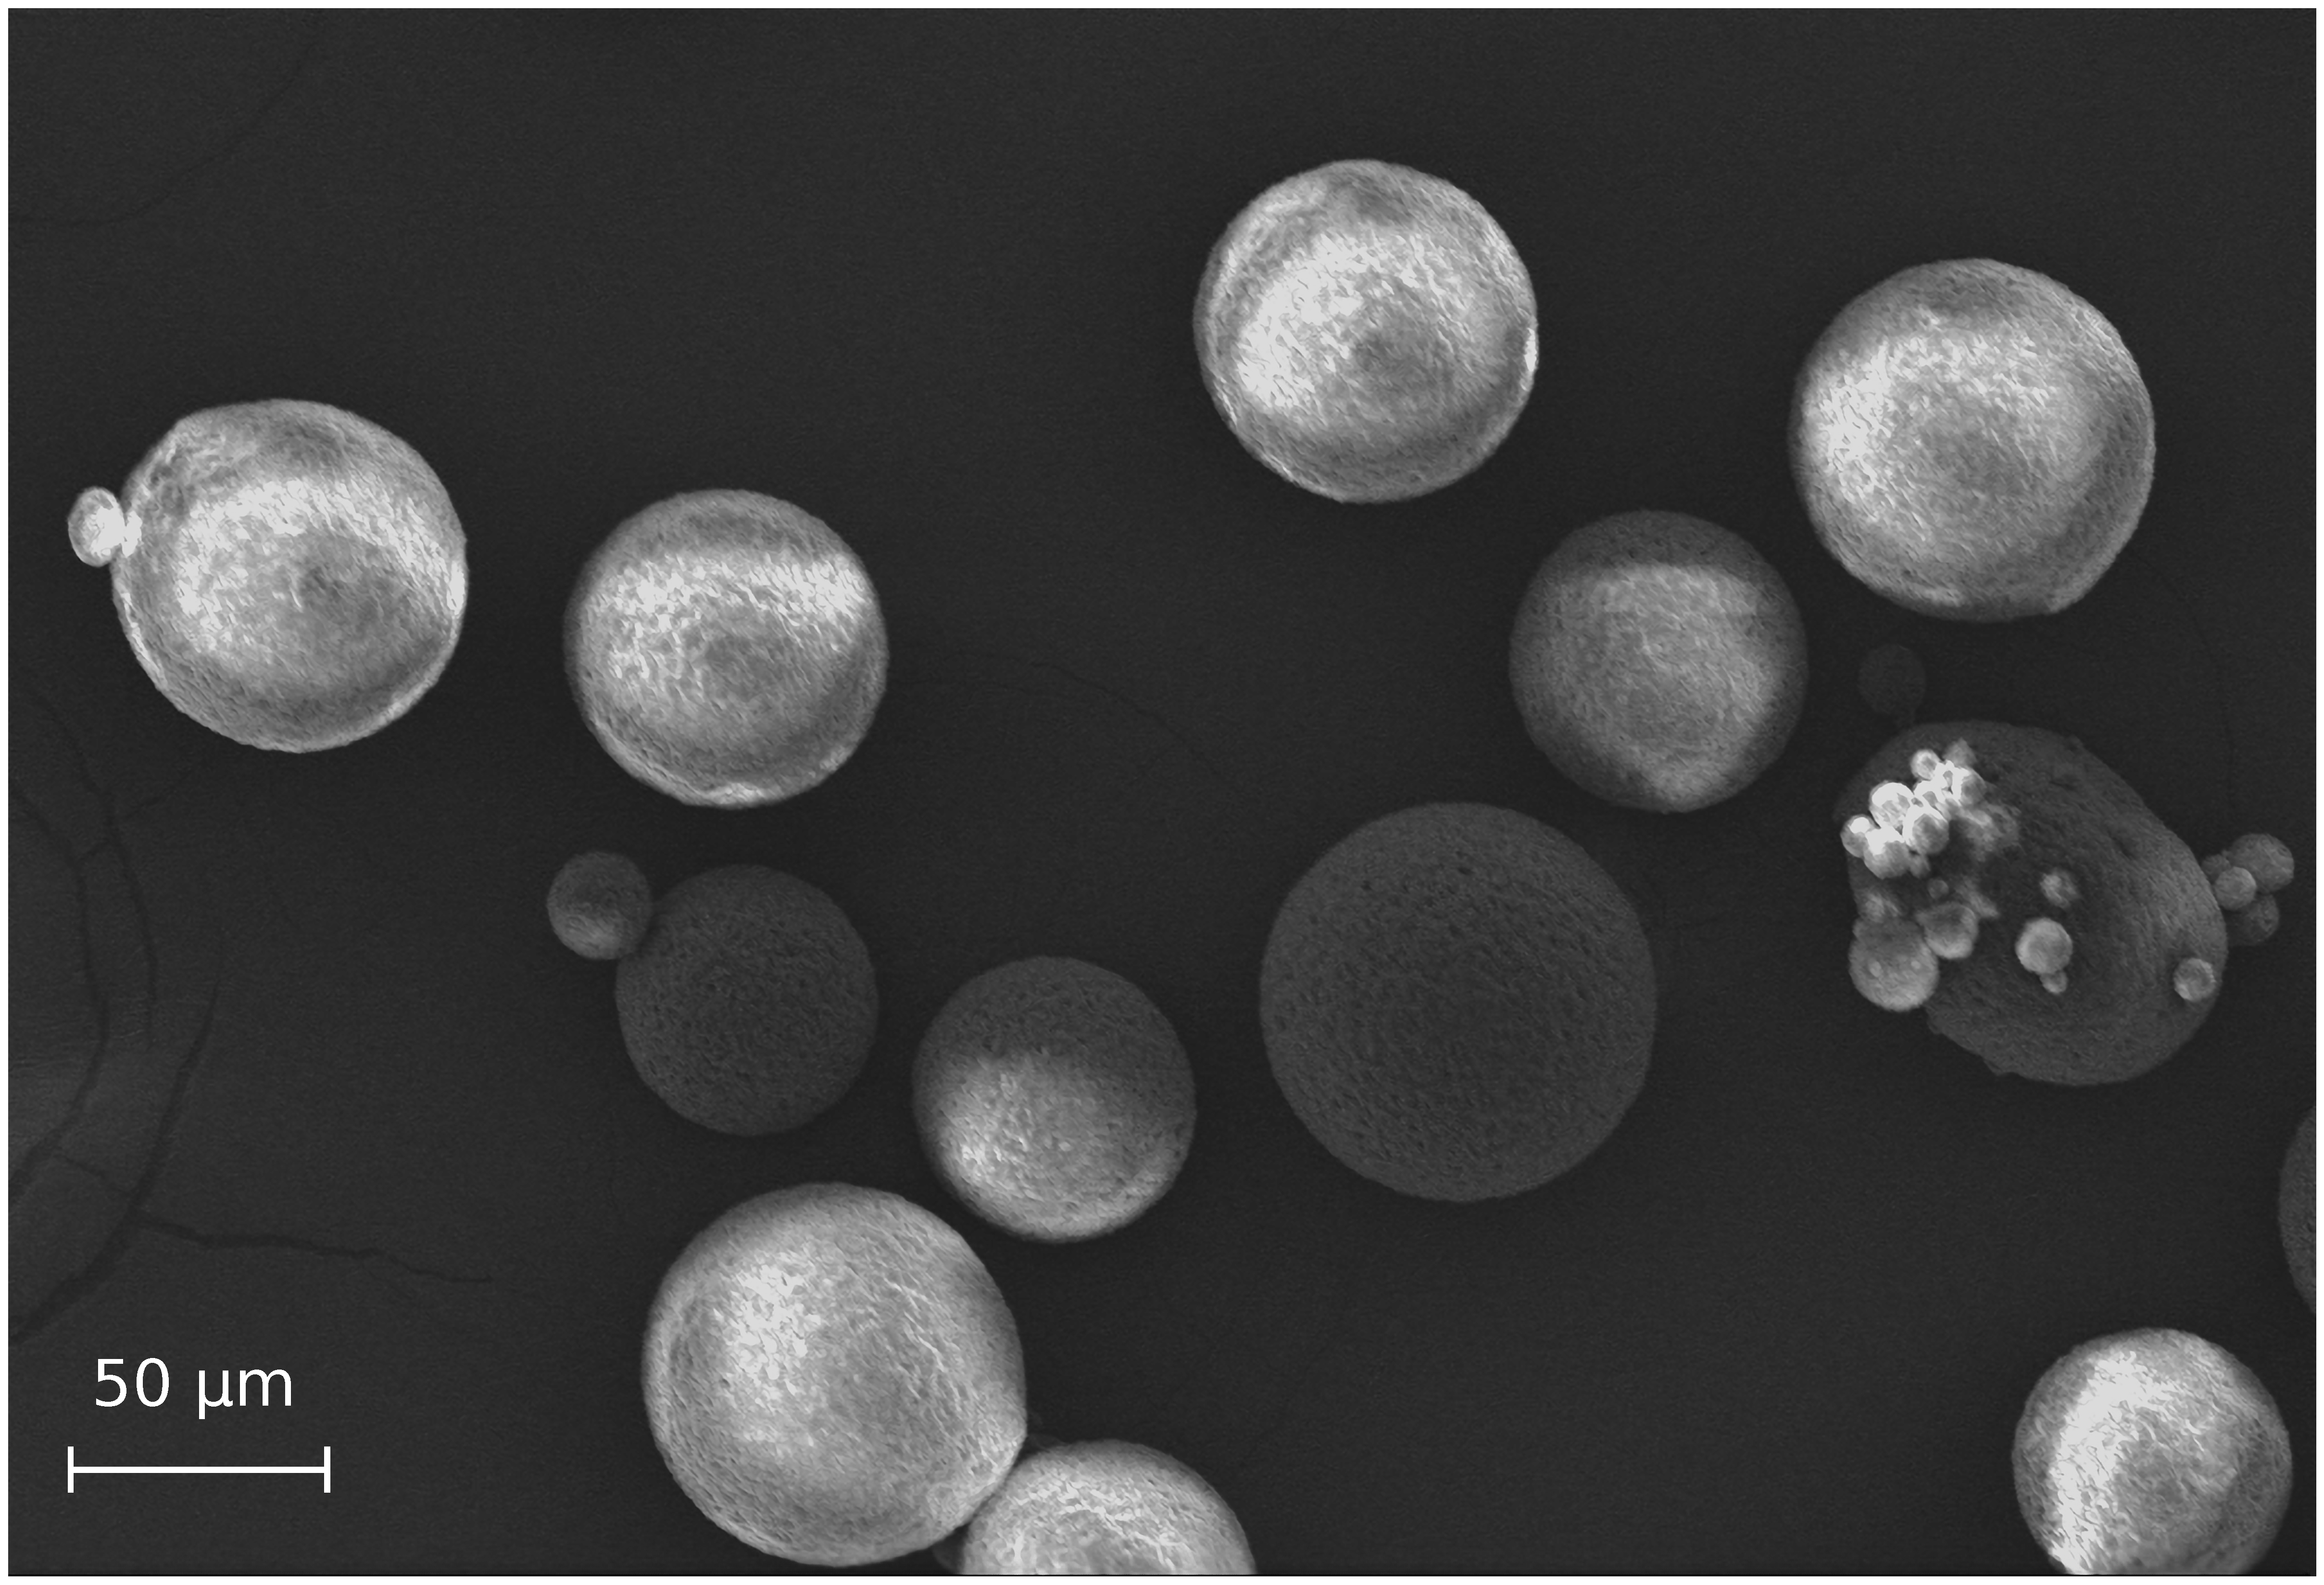
\includegraphics[width=\textwidth]{Pictures/SEM/Edited/04_01.eps}
          %    \caption{Enhanced SEM image, $SEM_{01}$ with a 461X magnification factor}
          %    \label{fig:SEM_01}
          %\end{figure}

          \begin{figure}[h!]
              \centering 
              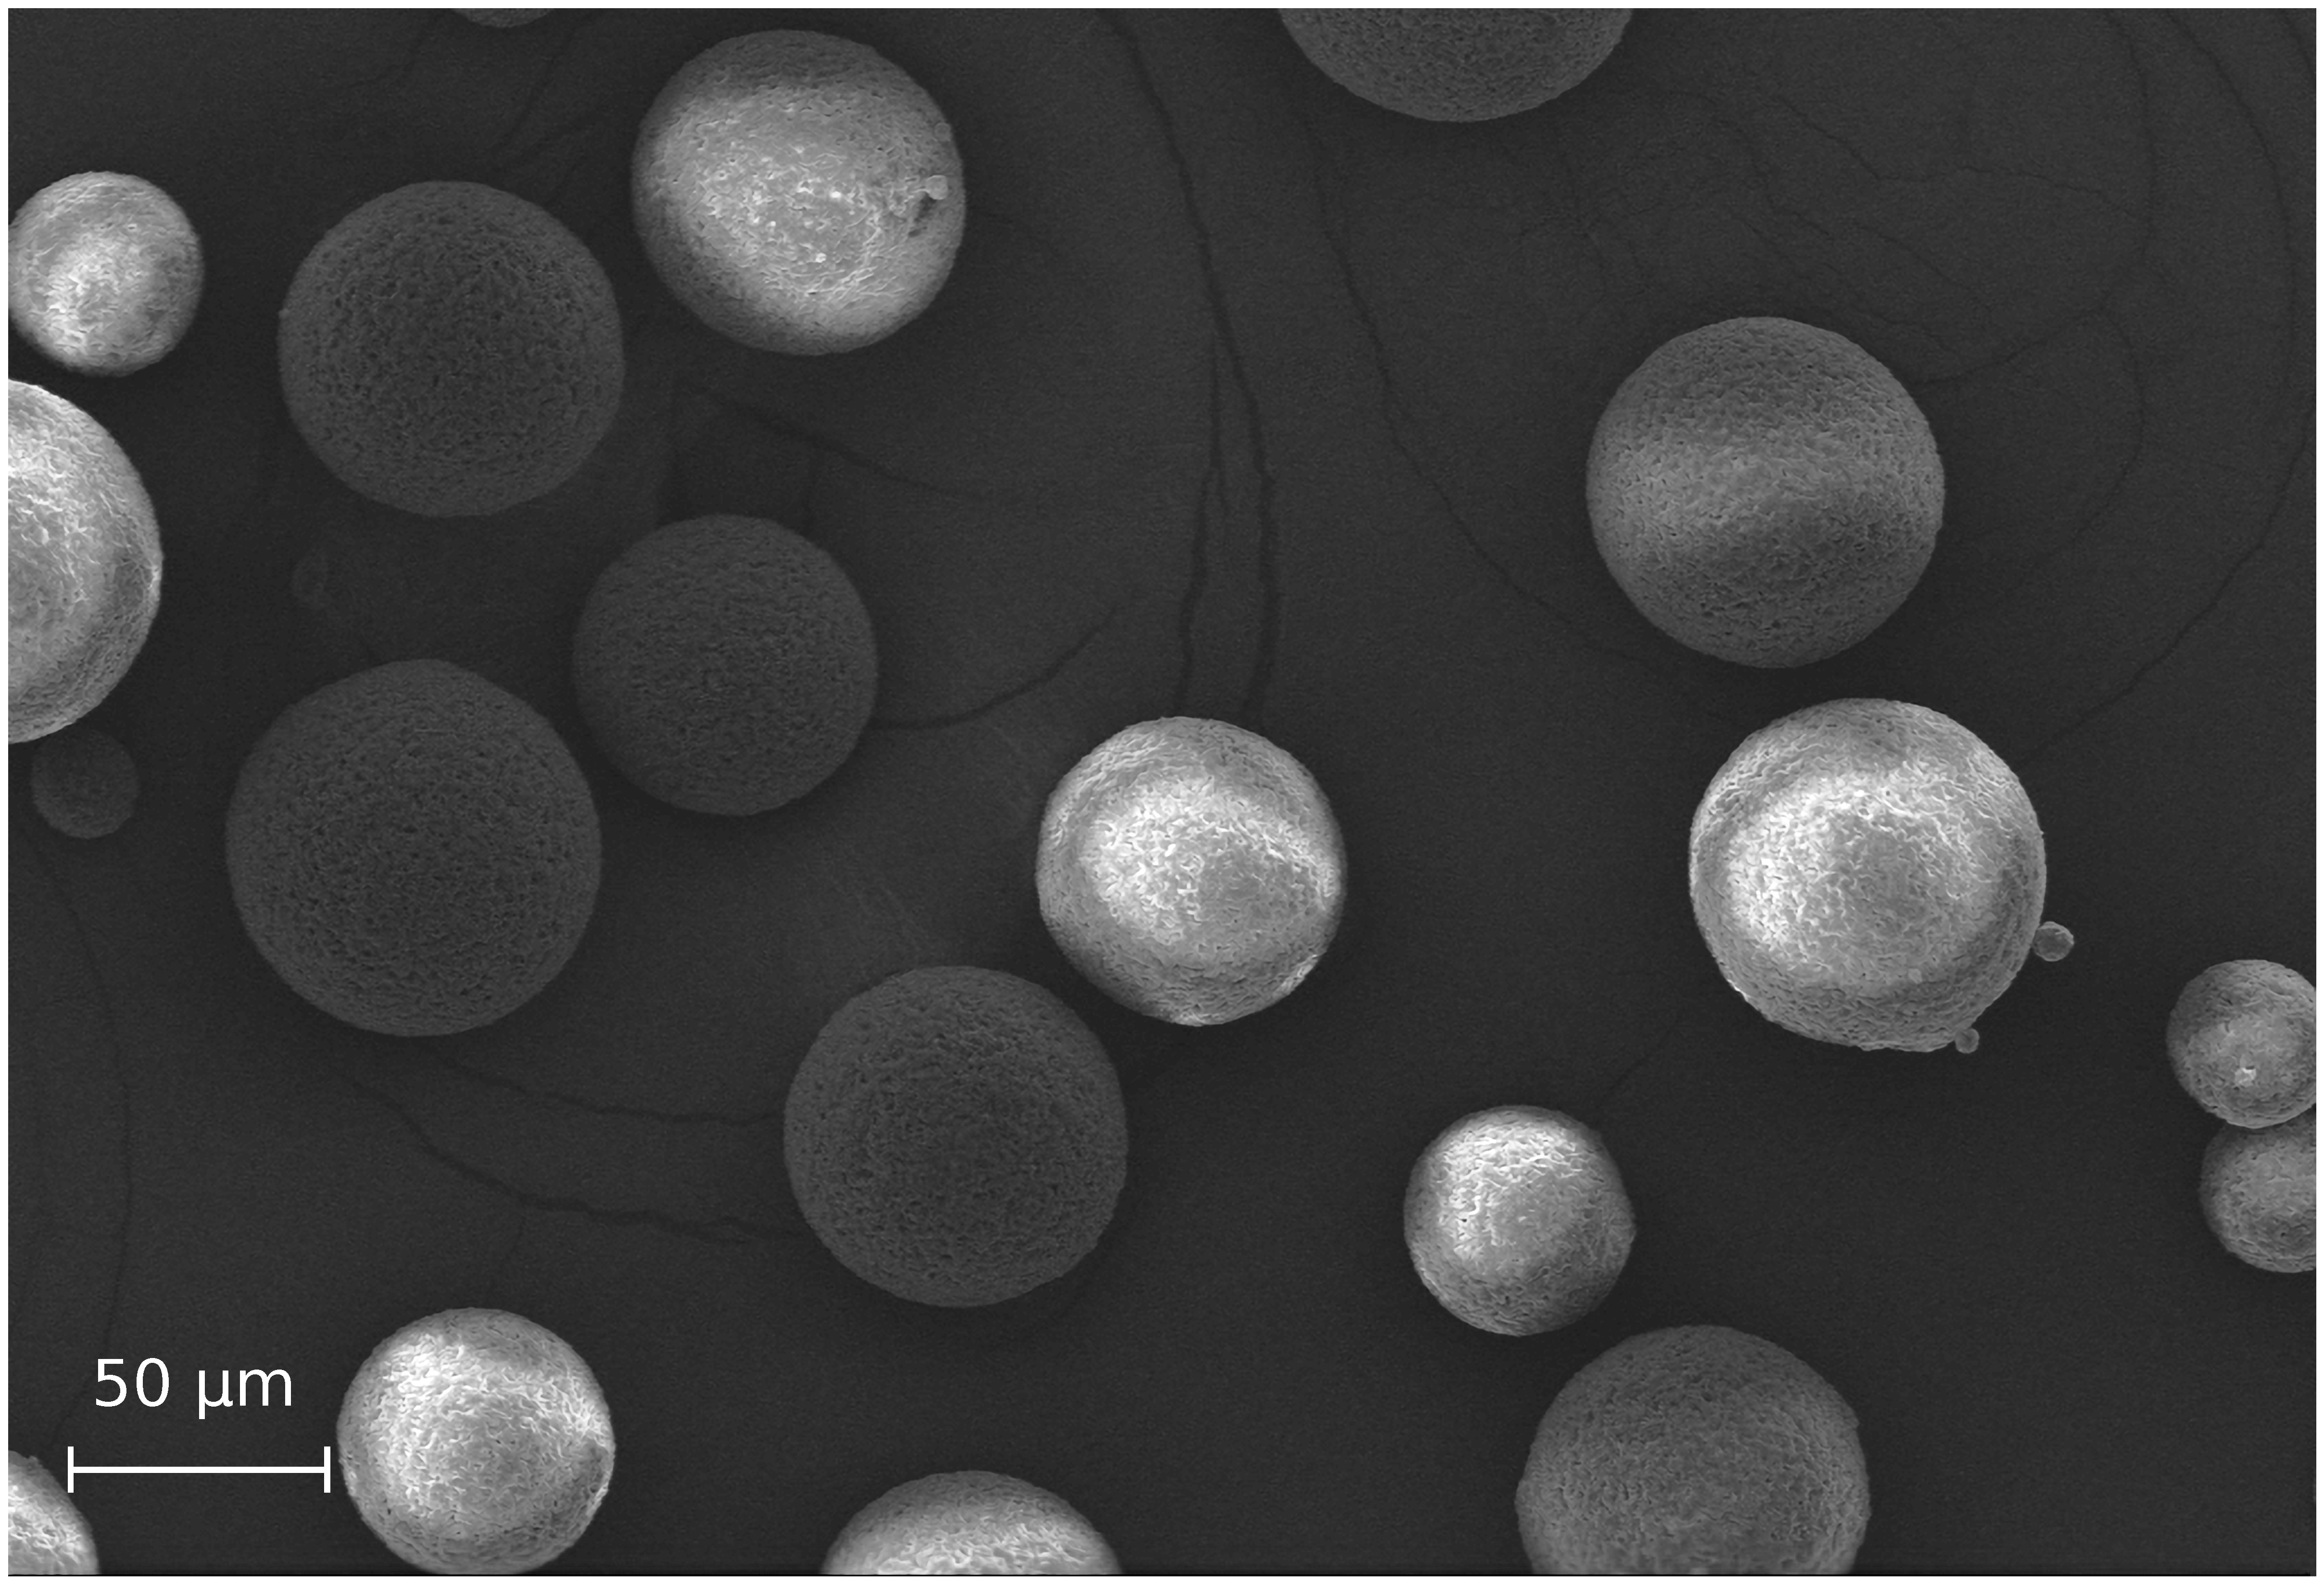
\includegraphics[width=\textwidth]{Pictures/SEM/Edited/04_02.eps}
              \caption{Enhanced SEM image, $SEM_{02}$ with a 461X magnification factor}
              \label{fig:SEM_02}
          \end{figure}

          \begin{figure}[h!]
              \centering 
              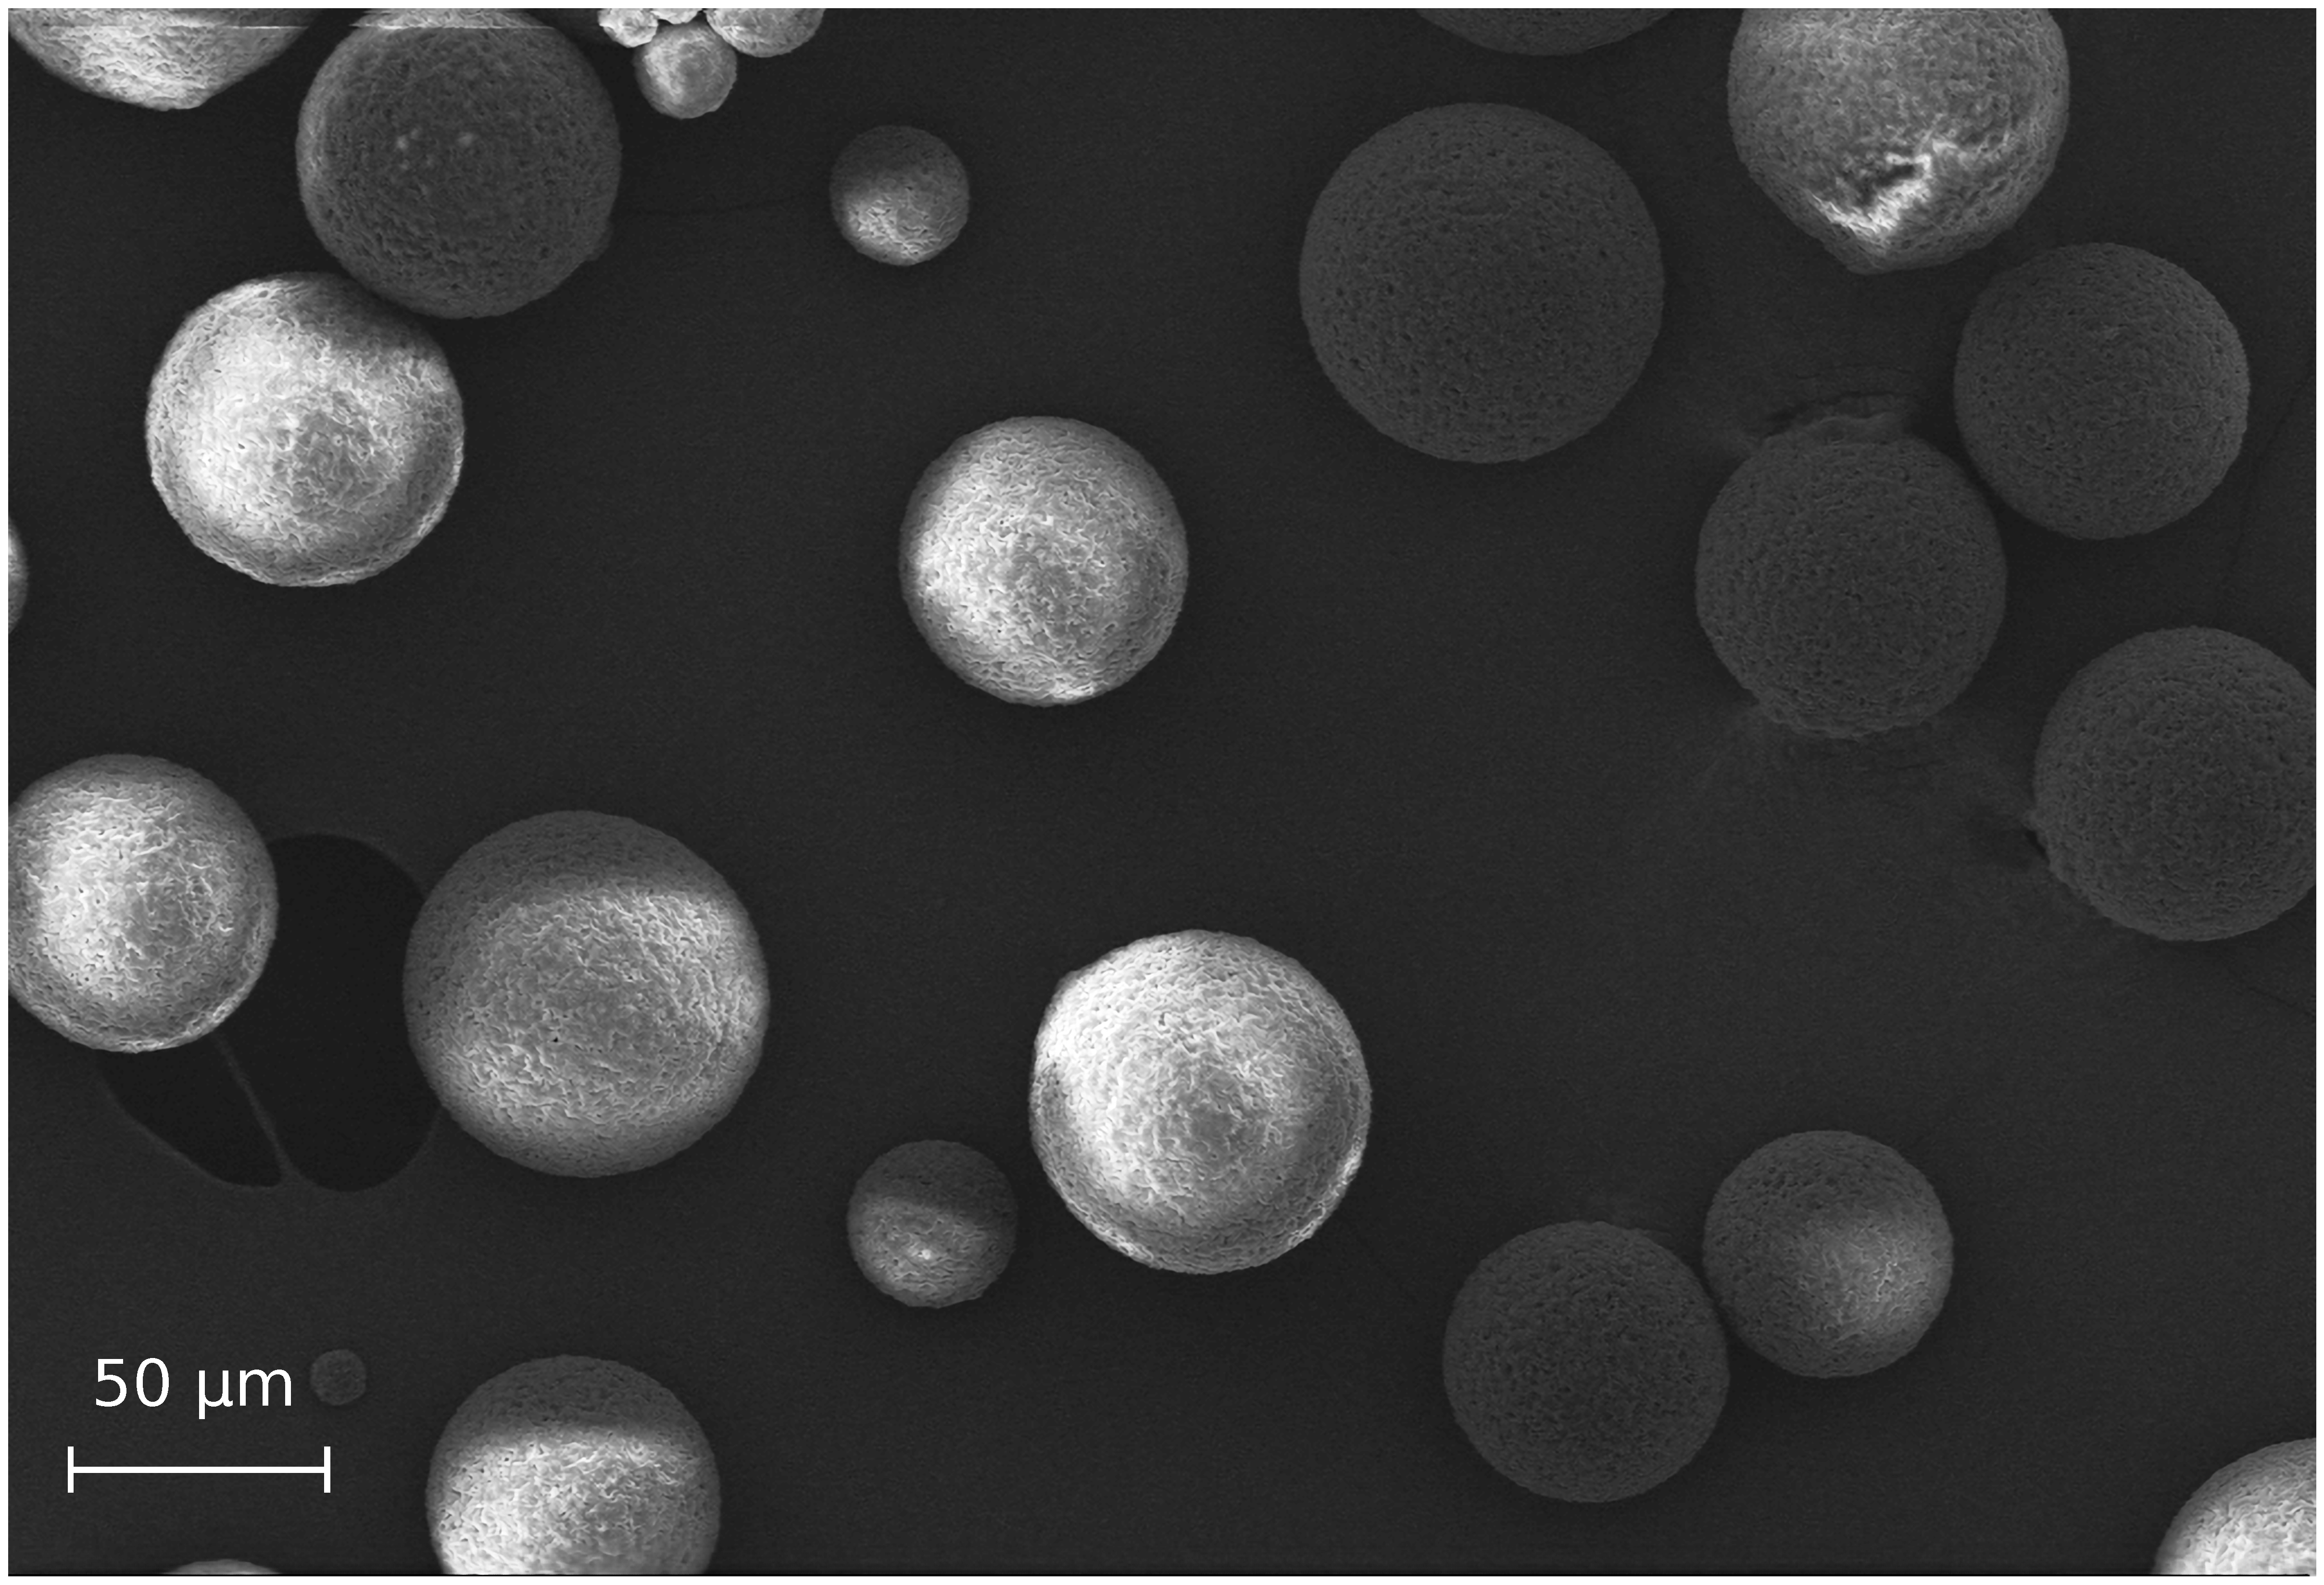
\includegraphics[width=\textwidth]{Pictures/SEM/Edited/04_03.eps}
              \caption{Enhanced SEM image, $SEM_{03}$ with a 461X magnification factor}
              \label{fig:SEM_03}
          \end{figure}

          %\begin{figure}[h!]
          %    \centering 
          %    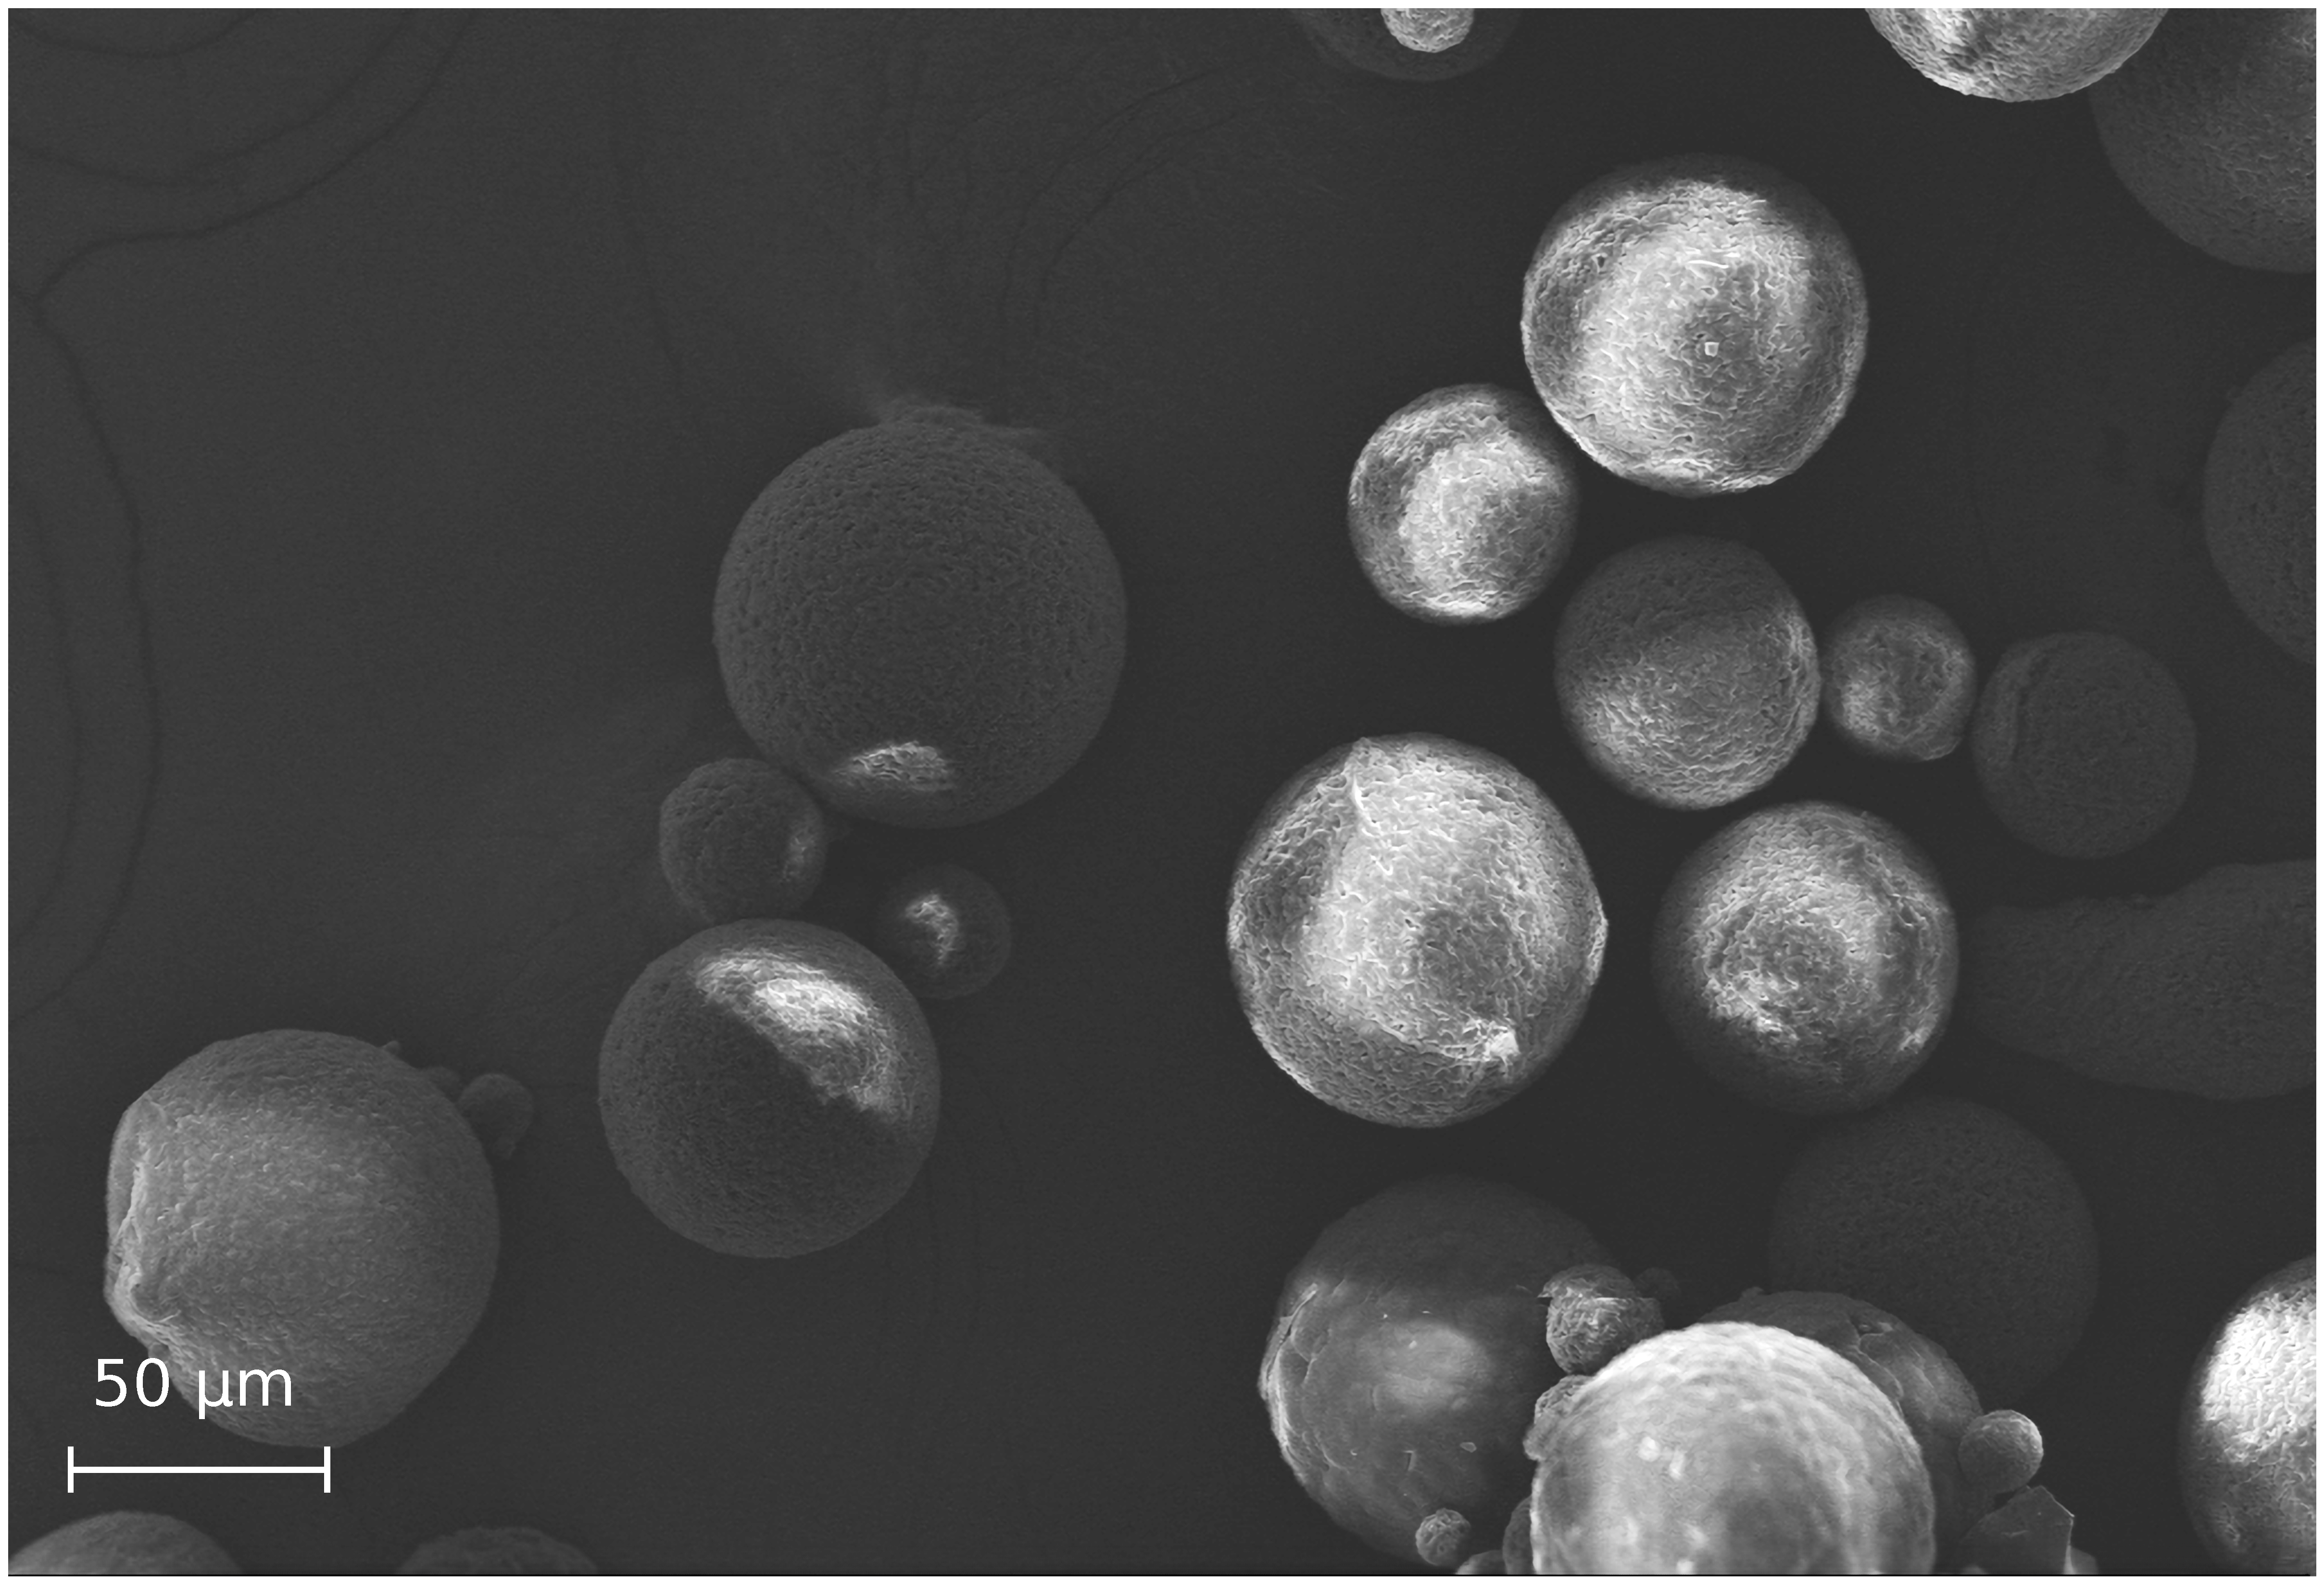
\includegraphics[width=\textwidth]{Pictures/SEM/Edited/05_03.eps}
          %    \caption{Enhanced SEM image, $SEM_{04}$ with a 461X magnification factor}
          %    \label{fig:SEM_04}
          %\end{figure}
      
          \begin{figure}[h!]
              \centering 
              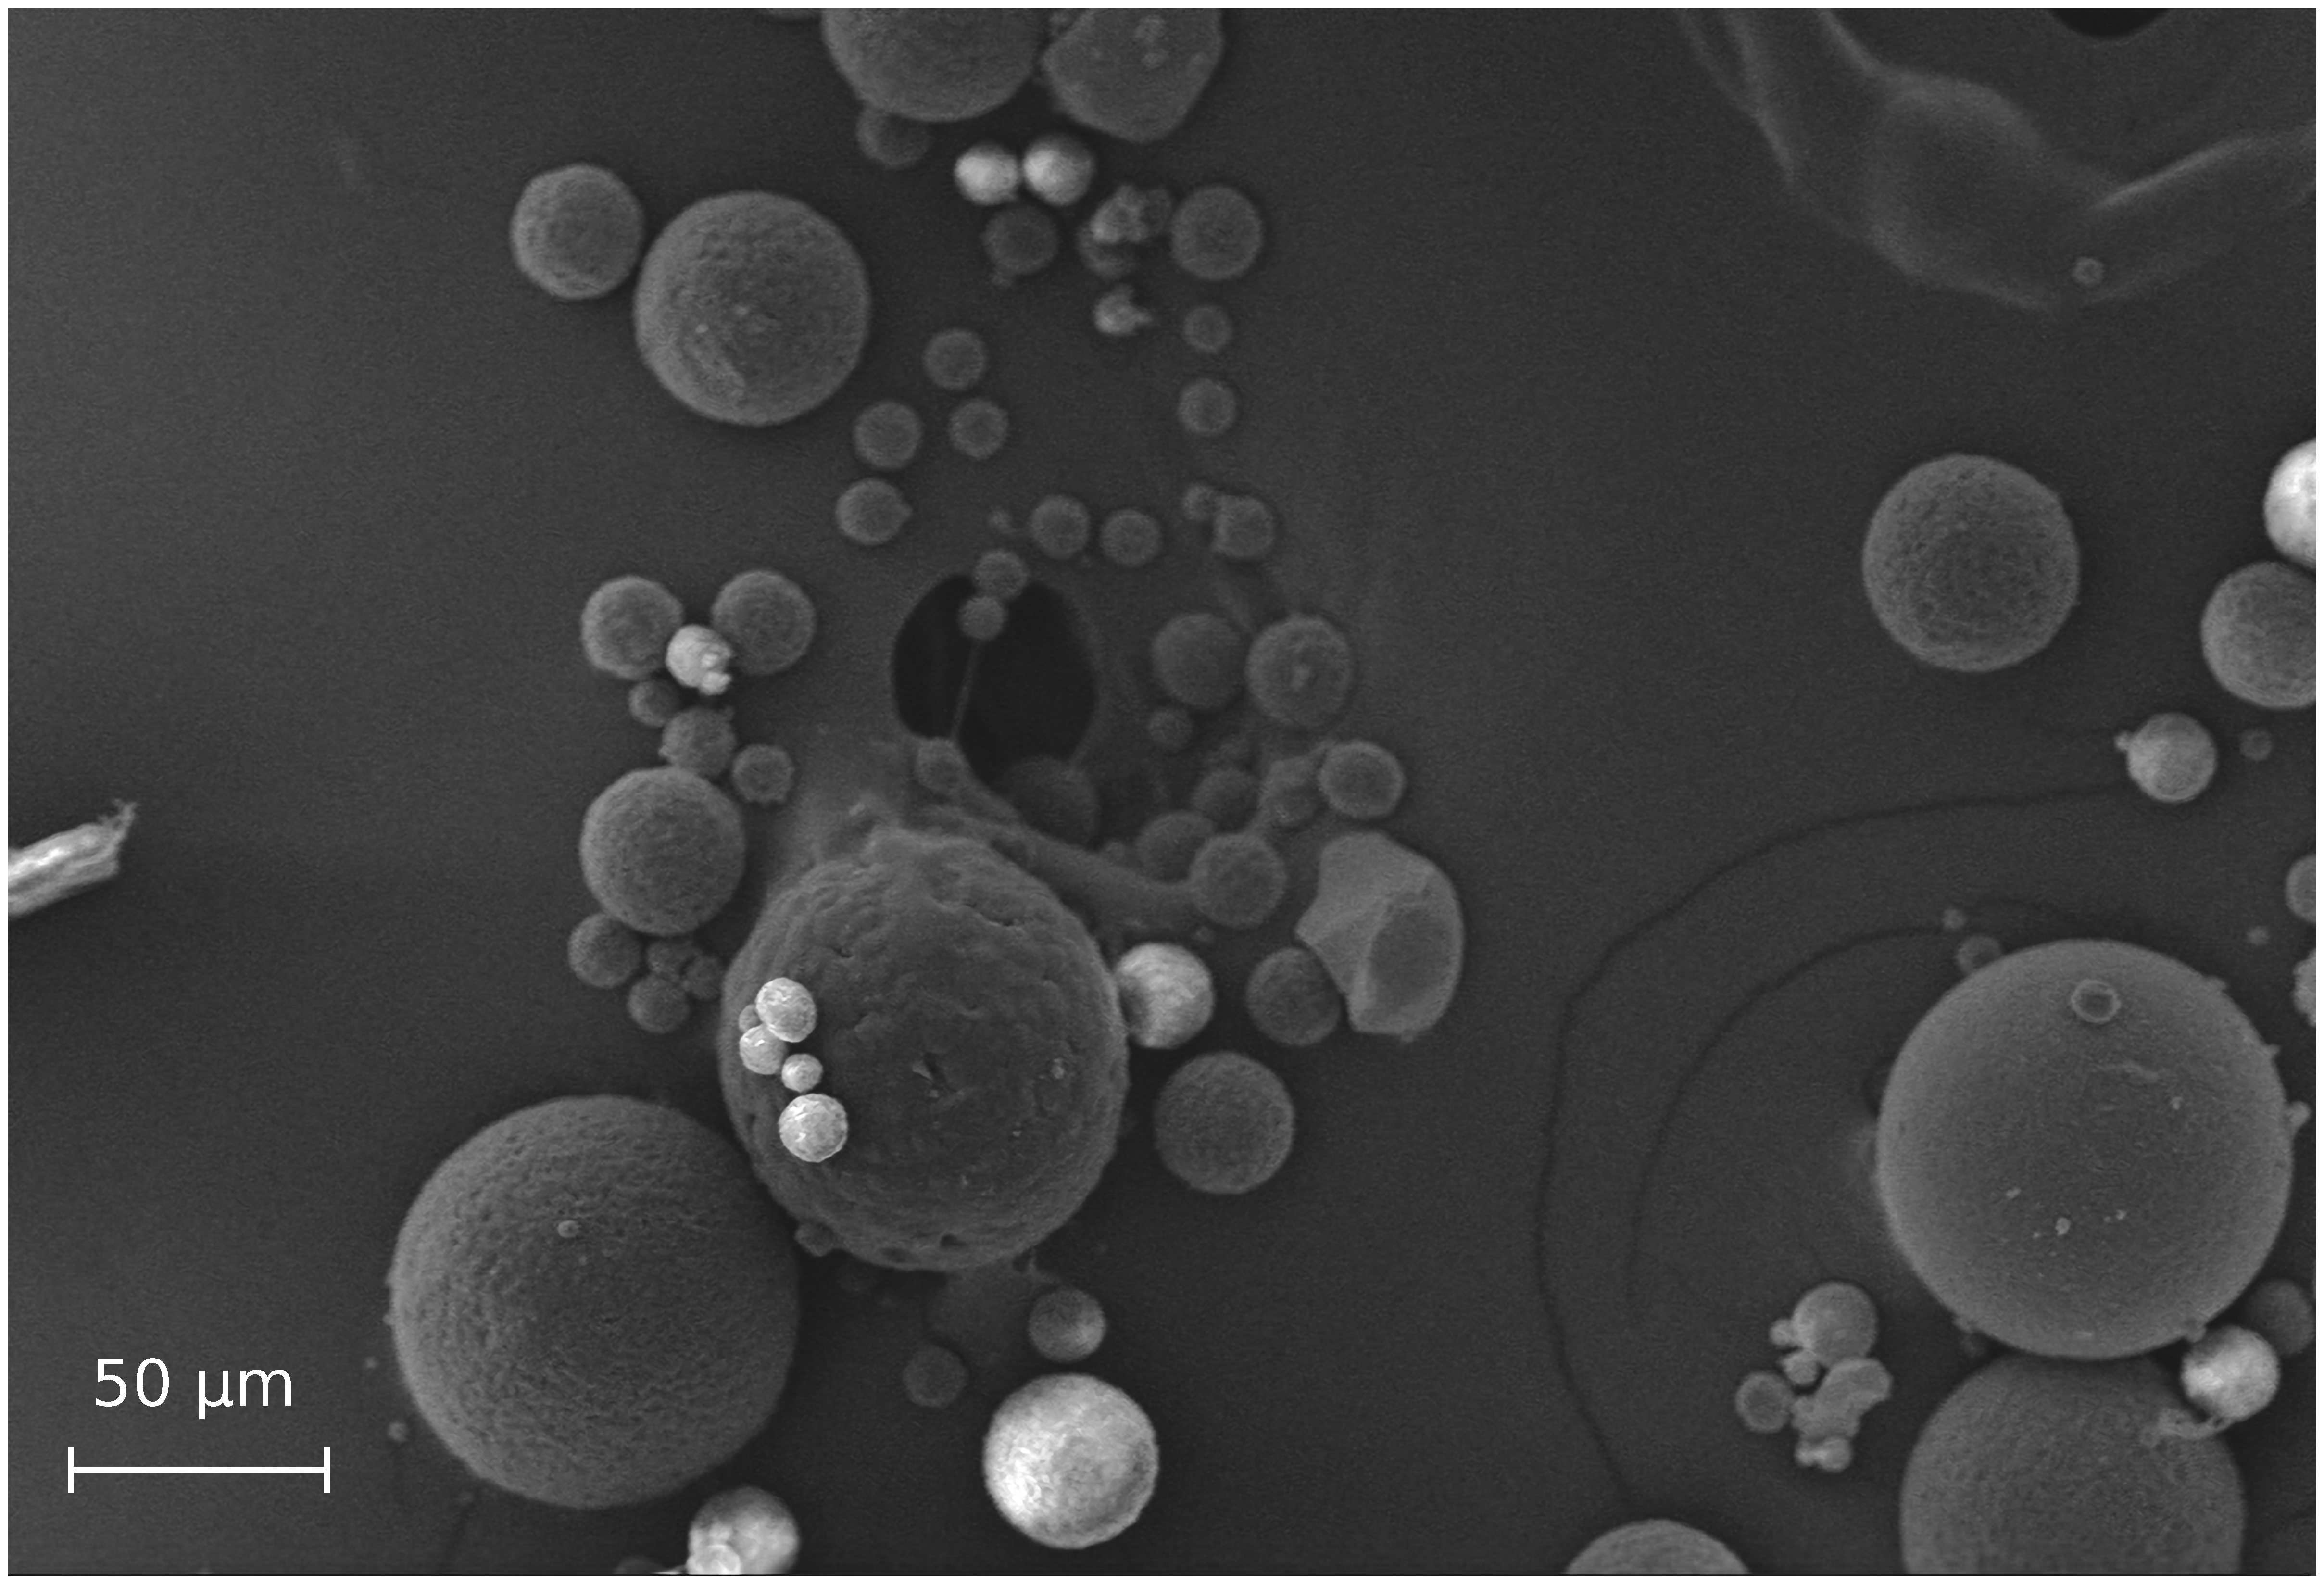
\includegraphics[width=\textwidth]{Pictures/SEM/Edited/06_01.eps}
              \caption{Enhanced SEM image, $SEM_{05}$ with a 461X magnification factor}
              \label{fig:SEM_05}
          \end{figure}
      
          %\begin{figure}[h!]
          %    \centering 
          %    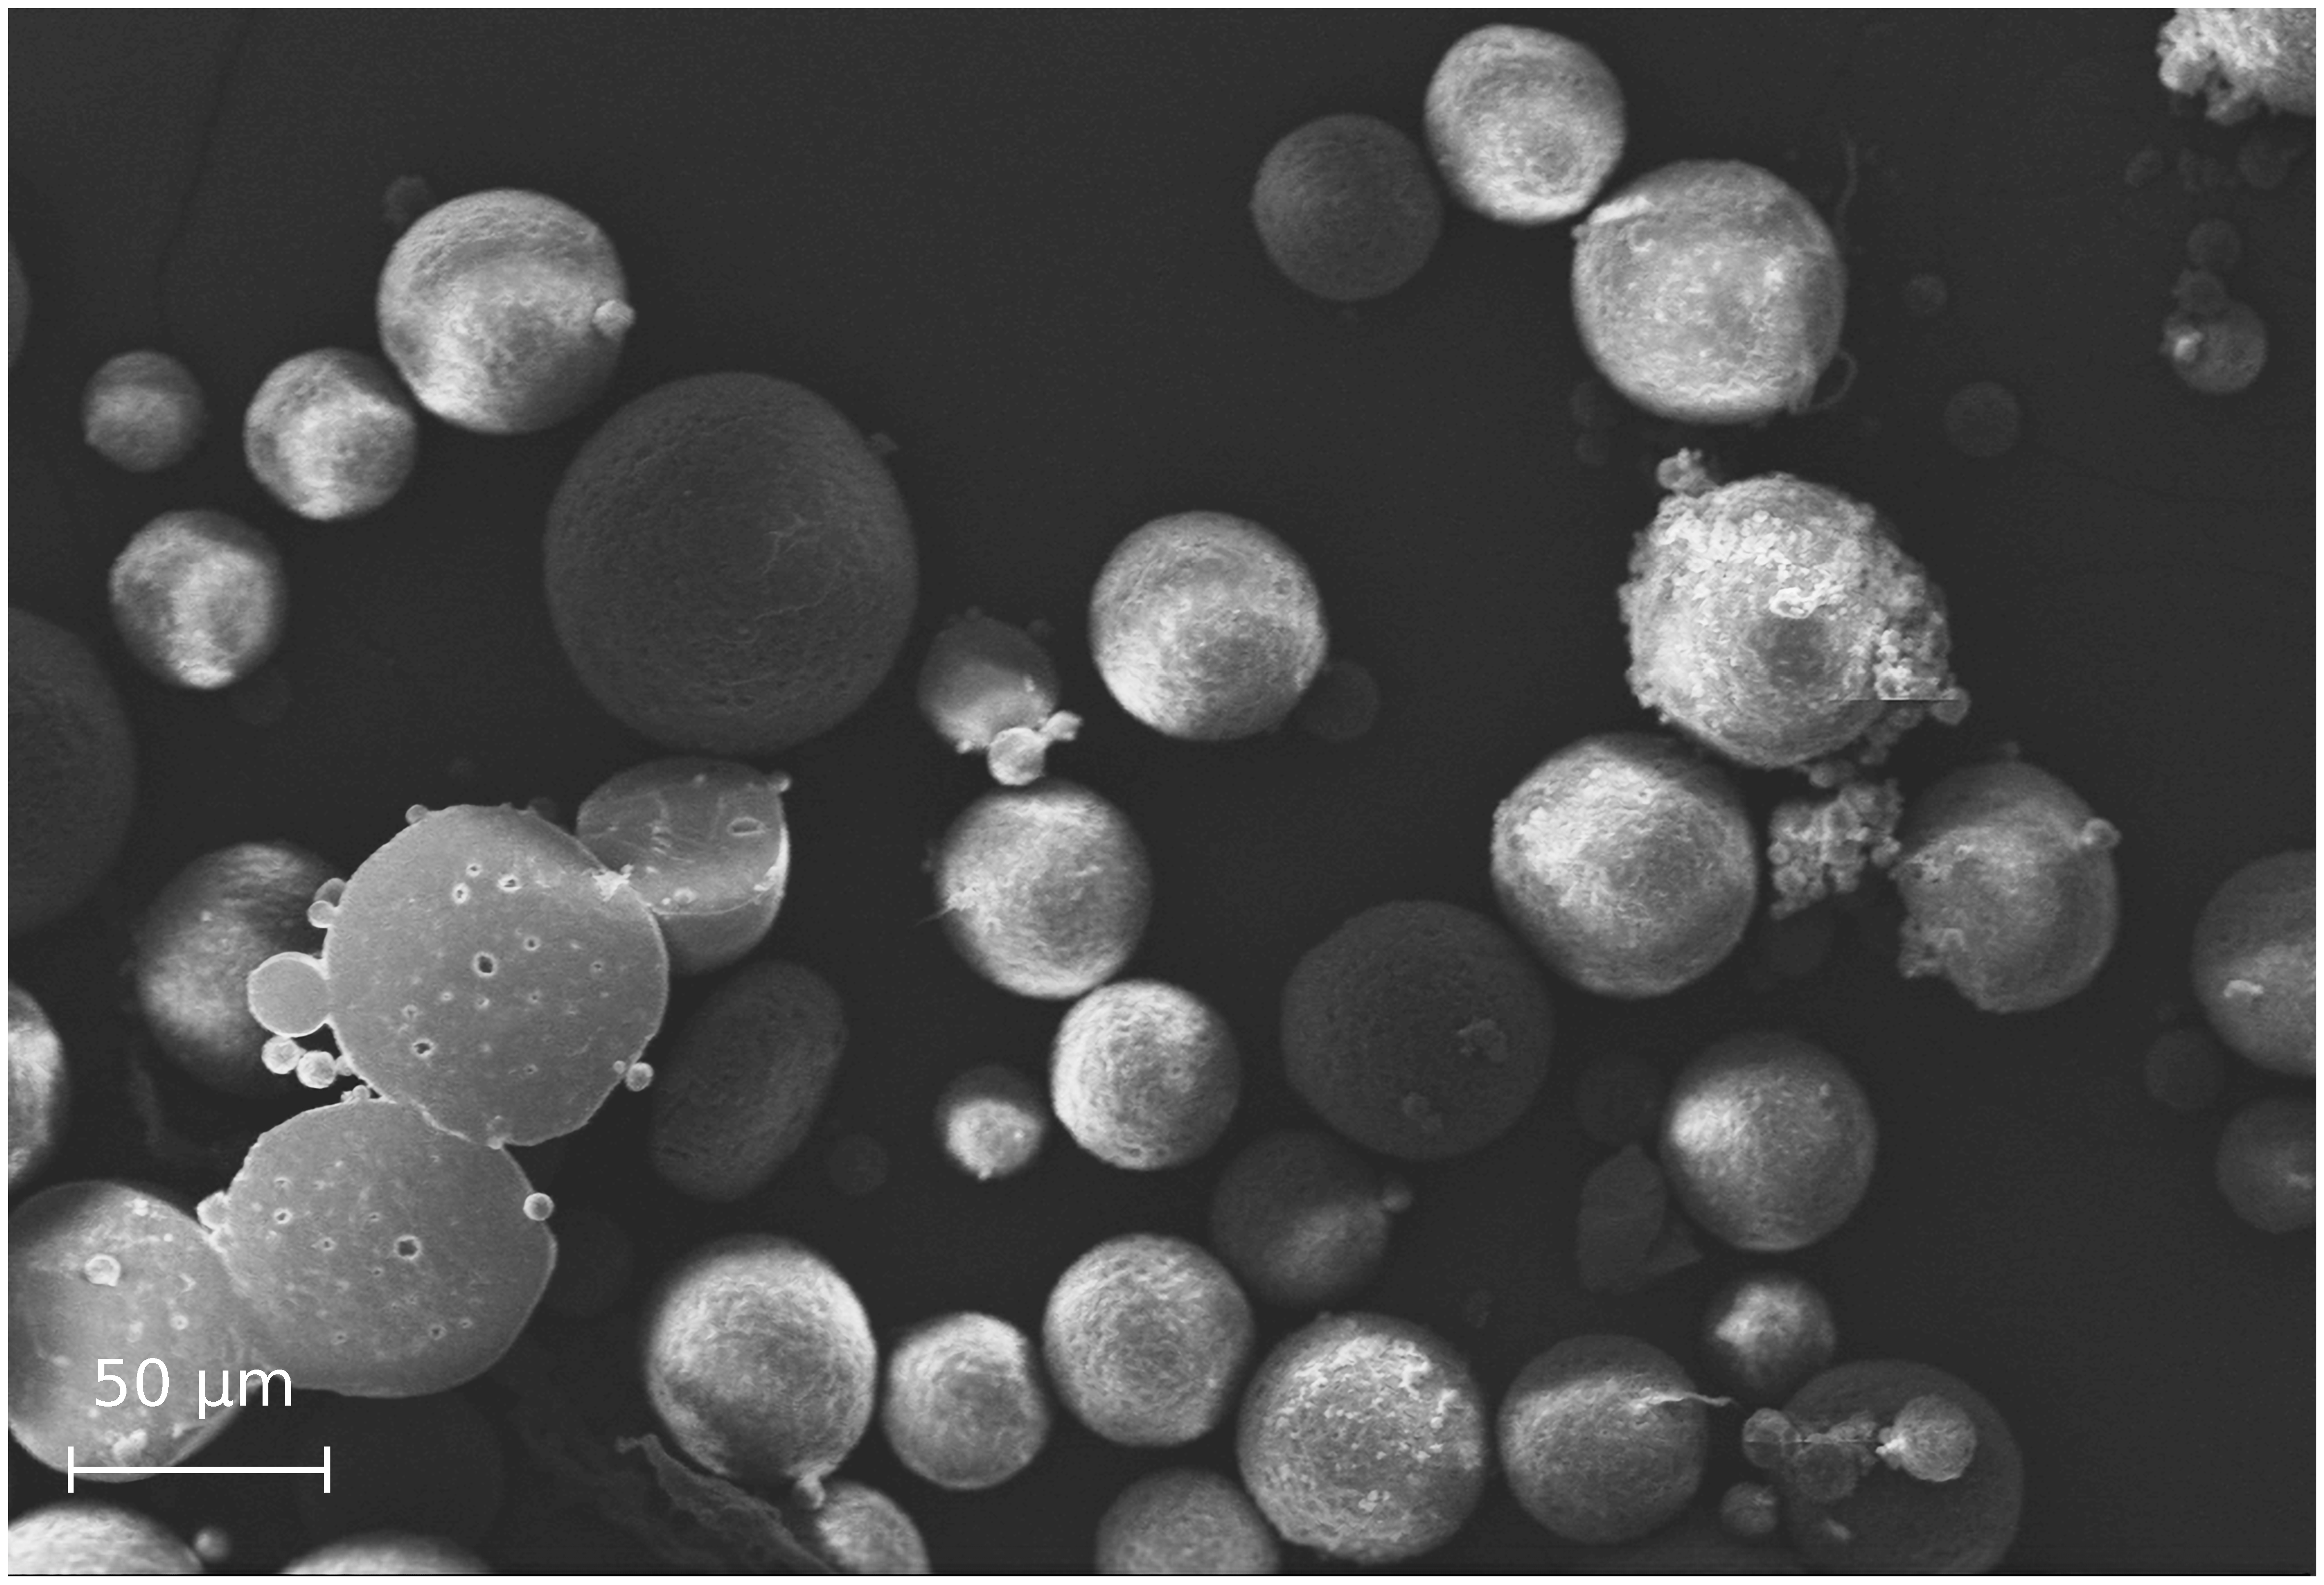
\includegraphics[width=\textwidth]{Pictures/SEM/Edited/06_03.eps}
          %    \caption{Enhanced SEM image, $SEM_{06}$ with a 461X magnification factor}
          %    \label{fig:SEM_06}
          %\end{figure}
      
          %\begin{figure}[h!]
          %    \centering 
          %    \includegraphics[width=\textwidth]{Pictures/SEM/Edited/sample_01.eps}
          %    \caption{Enhanced SEM image, $SEM_{07}$ with an 800X magnification factor}
          %    \label{fig:SEM_07}
          %\end{figure}
      
          \begin{figure}[h!]
              \centering 
              \includegraphics[width=\textwidth]{Pictures/SEM/Edited/sample_02.eps}
              \caption{Enhanced SEM image, $SEM_{08}$ with an 800X magnification factor}
              \label{fig:SEM_08}
          \end{figure}
      
          \begin{figure}[h!]
              \centering 
              \includegraphics[width=\textwidth]{Pictures/SEM/Edited/sample_03.eps}
              \caption{Enhanced SEM image, $SEM_{09}$ with an 800X magnification factor}
              \label{fig:SEM_09}
          \end{figure}

          %\begin{figure}[h!]
          %    \centering 
          %    \includegraphics[width=\textwidth]{Pictures/SEM/Edited/sample_04.eps}
          %    \caption{Enhanced SEM image, $SEM_{10}$ with a 400X magnification factor}
          %    \label{fig:SEM_10}
          %\end{figure}
%
          %\begin{figure}[h!]
          %    \centering 
          %    \includegraphics[width=\textwidth]{Pictures/SEM/Edited/sample_05.eps}
          %    \caption{Enhanced SEM image, $SEM_{11}$ with a 400X magnification factor}
          %    \label{fig:SEM_11}
          %\end{figure}

          \begin{figure}[h!]
              \centering 
              \includegraphics[width=\textwidth]{Pictures/SEM/Edited/sample_06.eps}
              \caption{Enhanced SEM image, $SEM_{12}$ with a 400X magnification factor}
              \label{fig:SEM_12}
          \end{figure}

    \clearpage

    \subsection{Granulometry Results\label{Granulometry_results}}
      
      The output data has been analyzed and the most meaningful features have been plotted as vector images using \textit{Labplot} \autocites{Labplot} and 
      postprocessed with \textit{Inkscape} \autocites{Inkscape}. \\ 
  
      %\begin{figure}[h!]
      %    \centering
      %    \begin{subfigure}[a]{\textwidth}
      %        \centering
      %        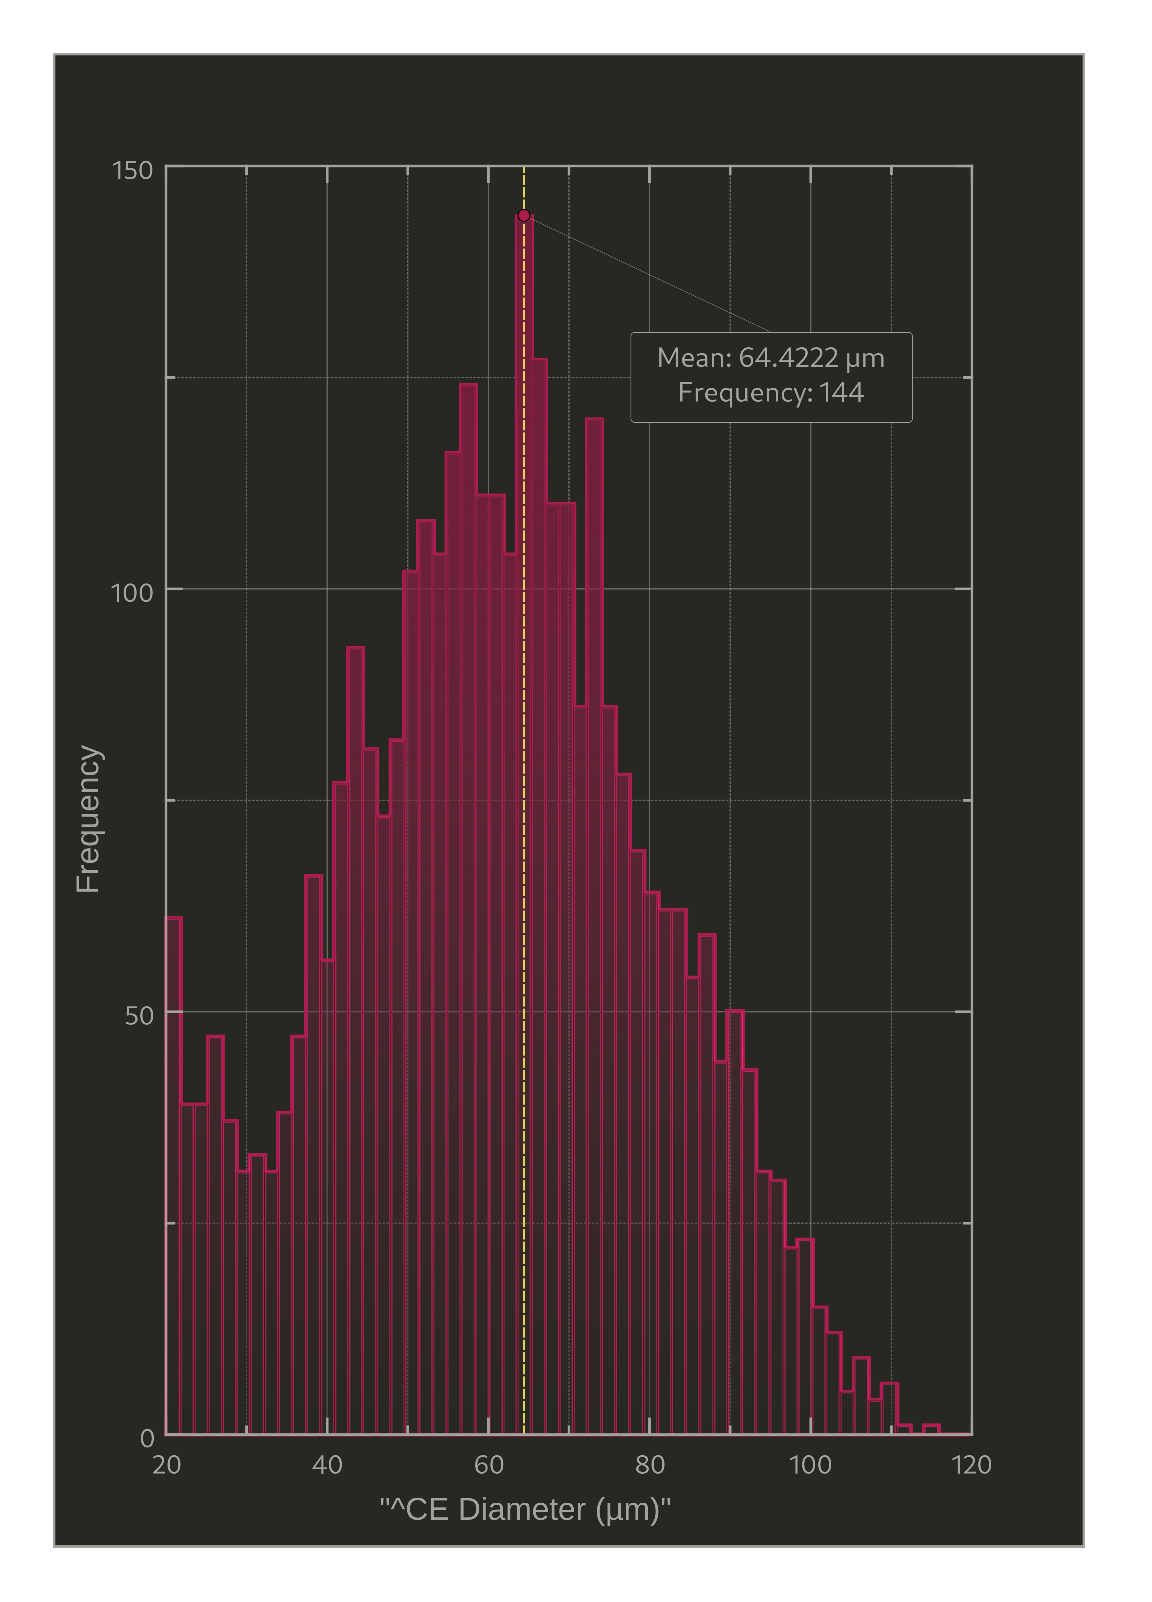
\includegraphics[width=\textwidth]{Pictures/Granulometry_plots/Histogram_CE-DIAM.eps}
      %        \caption{Particle Size Distribution}
      %        \label{fig:particle_size_distribution}
      %    \end{subfigure}
      %    \vfill
      %    \begin{subfigure}[b]{\textwidth}
      %        \centering
      %        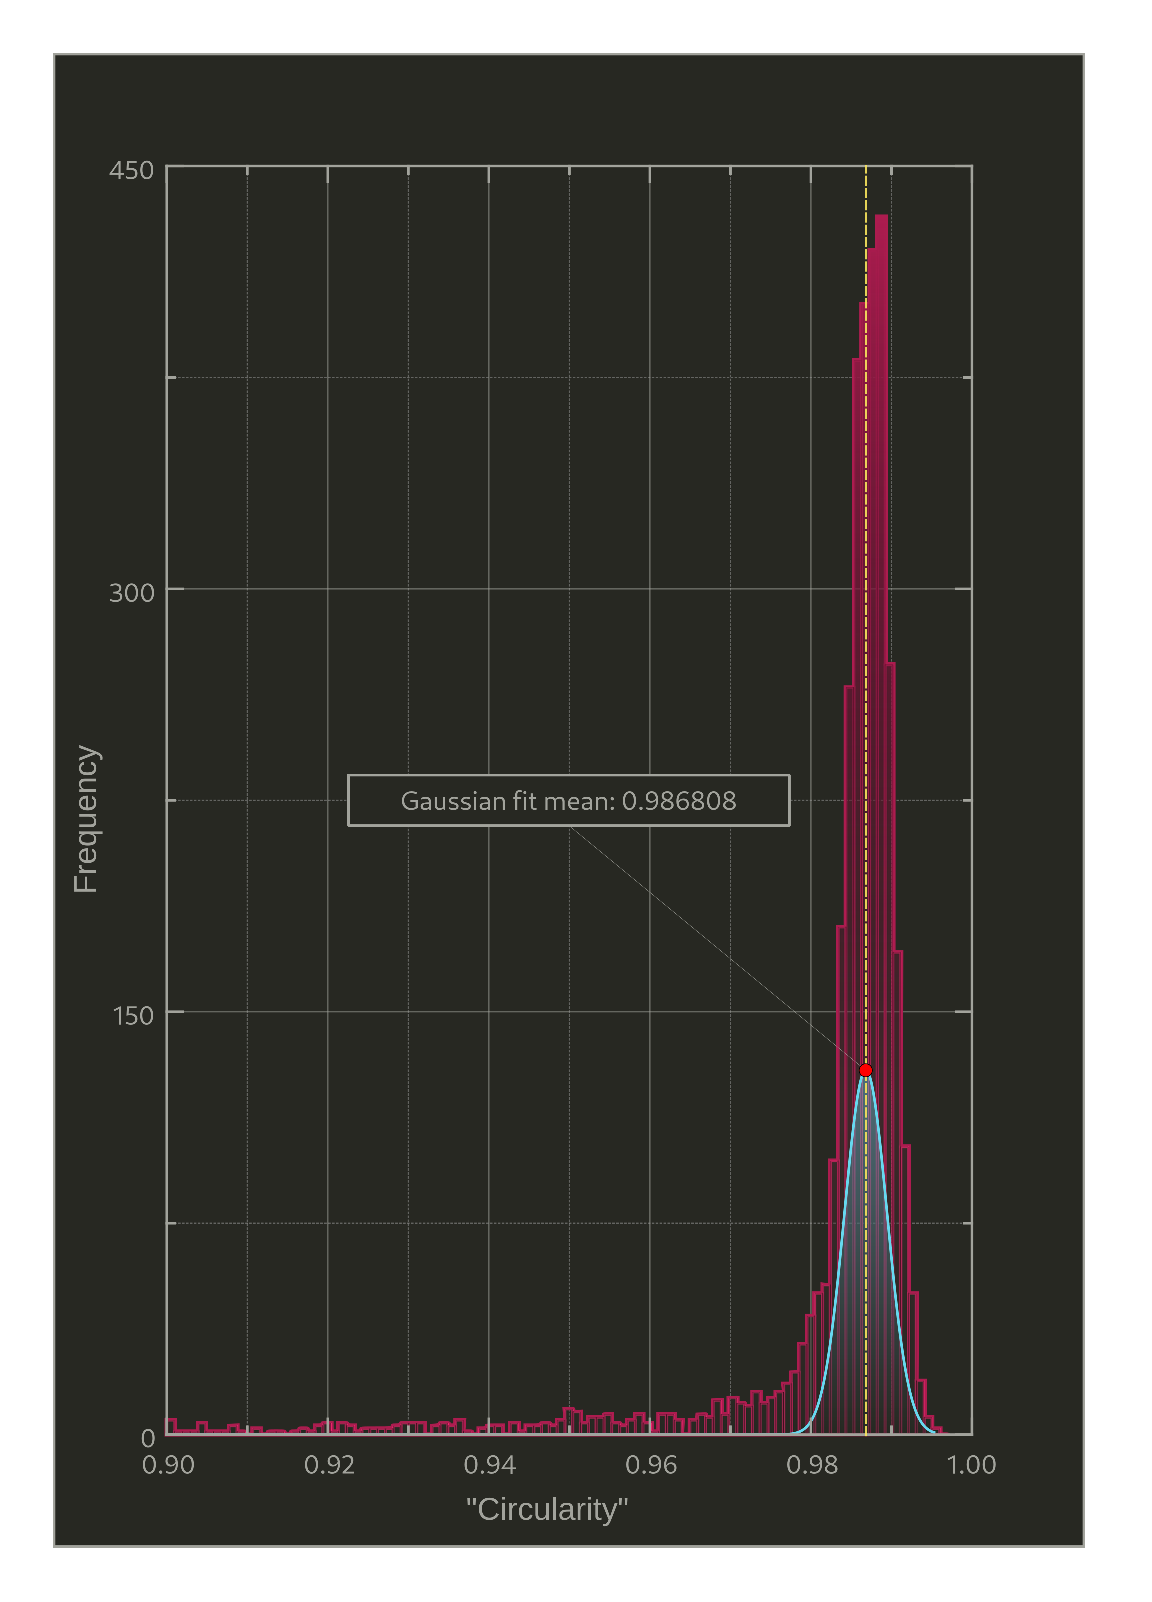
\includegraphics[width=\textwidth]{Pictures/Granulometry_plots/Histogram_Circularity.eps}
      %        \caption{Particle Circularity Distribution}
      %        \label{fig:circularity_distribution}
      %    \end{subfigure}
      %    \caption{Granulometry analysis of the powder sample}
      %    \label{fig:granulometry_analysis}
      %\end{figure}

        \begin{figure}[h!]
            \centering
            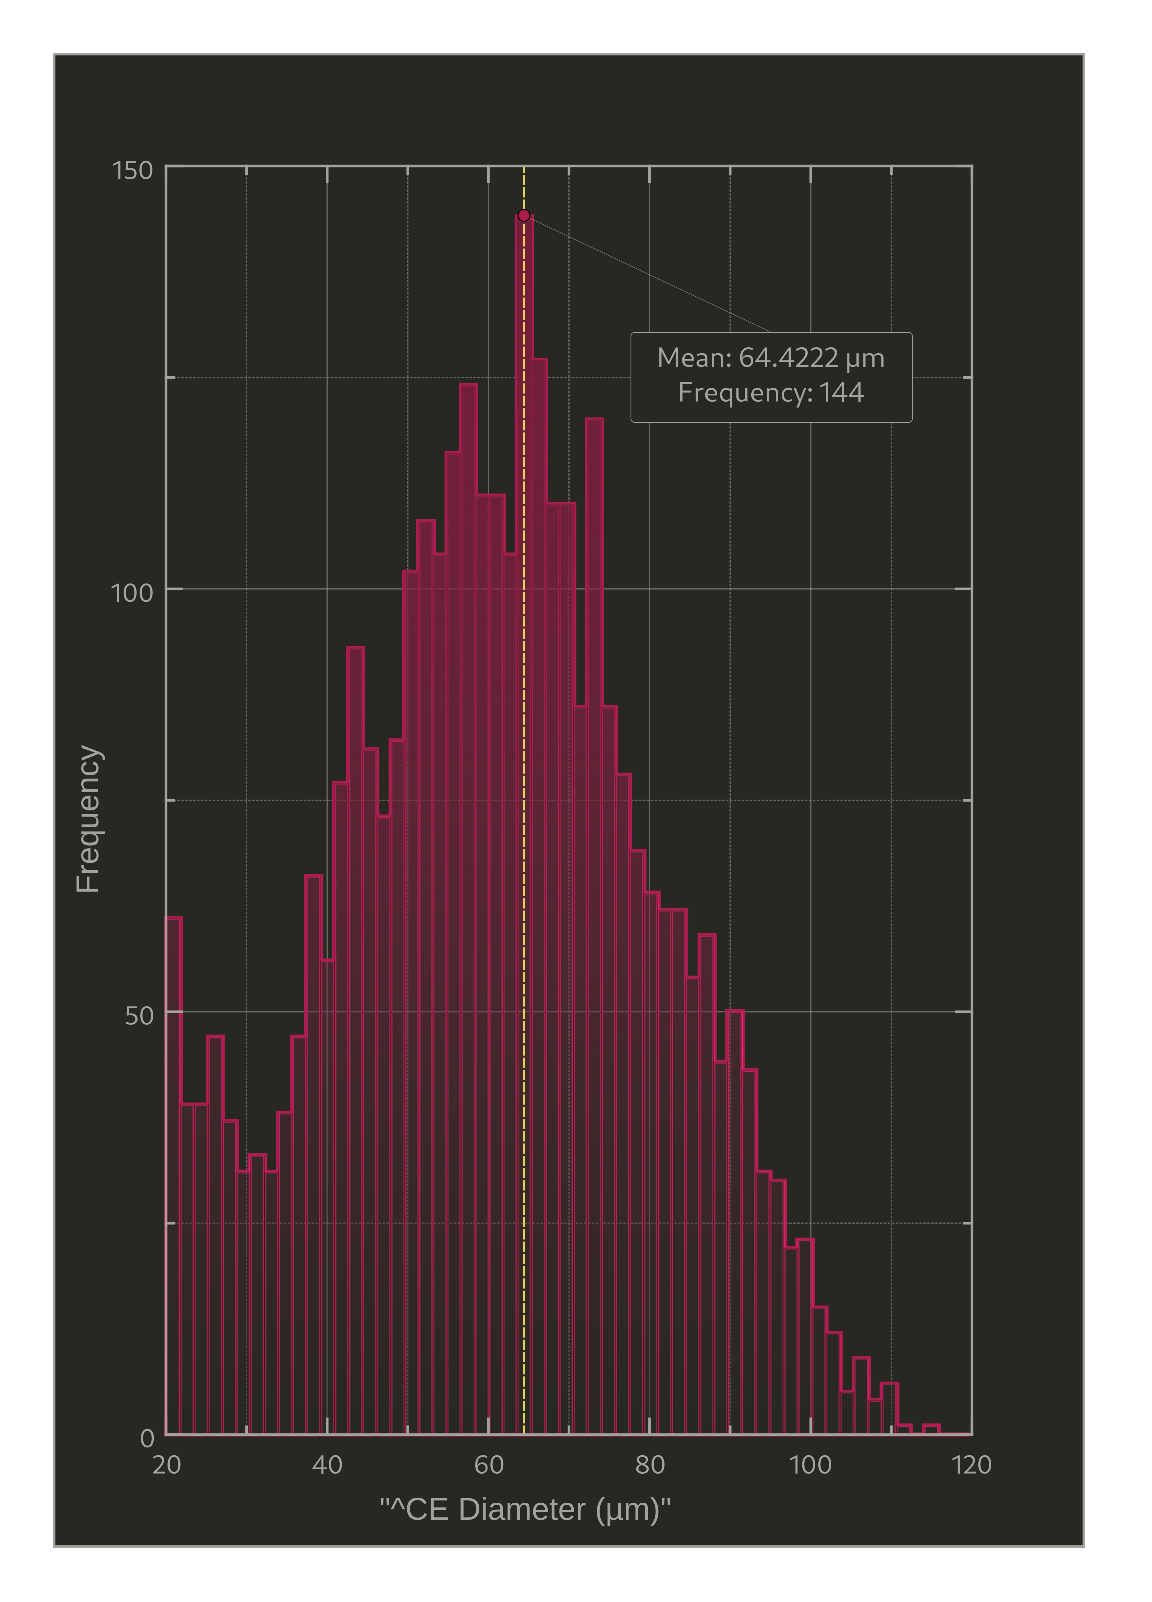
\includegraphics[width=0.9\textwidth]{Pictures/Granulometry_plots/Histogram_CE-DIAM.eps}
            \caption{Particle Size Distribution of a powder sample}
            \label{fig:particle_size_distribution}
        \end{figure}

        \begin{figure}[h!]
            \centering
            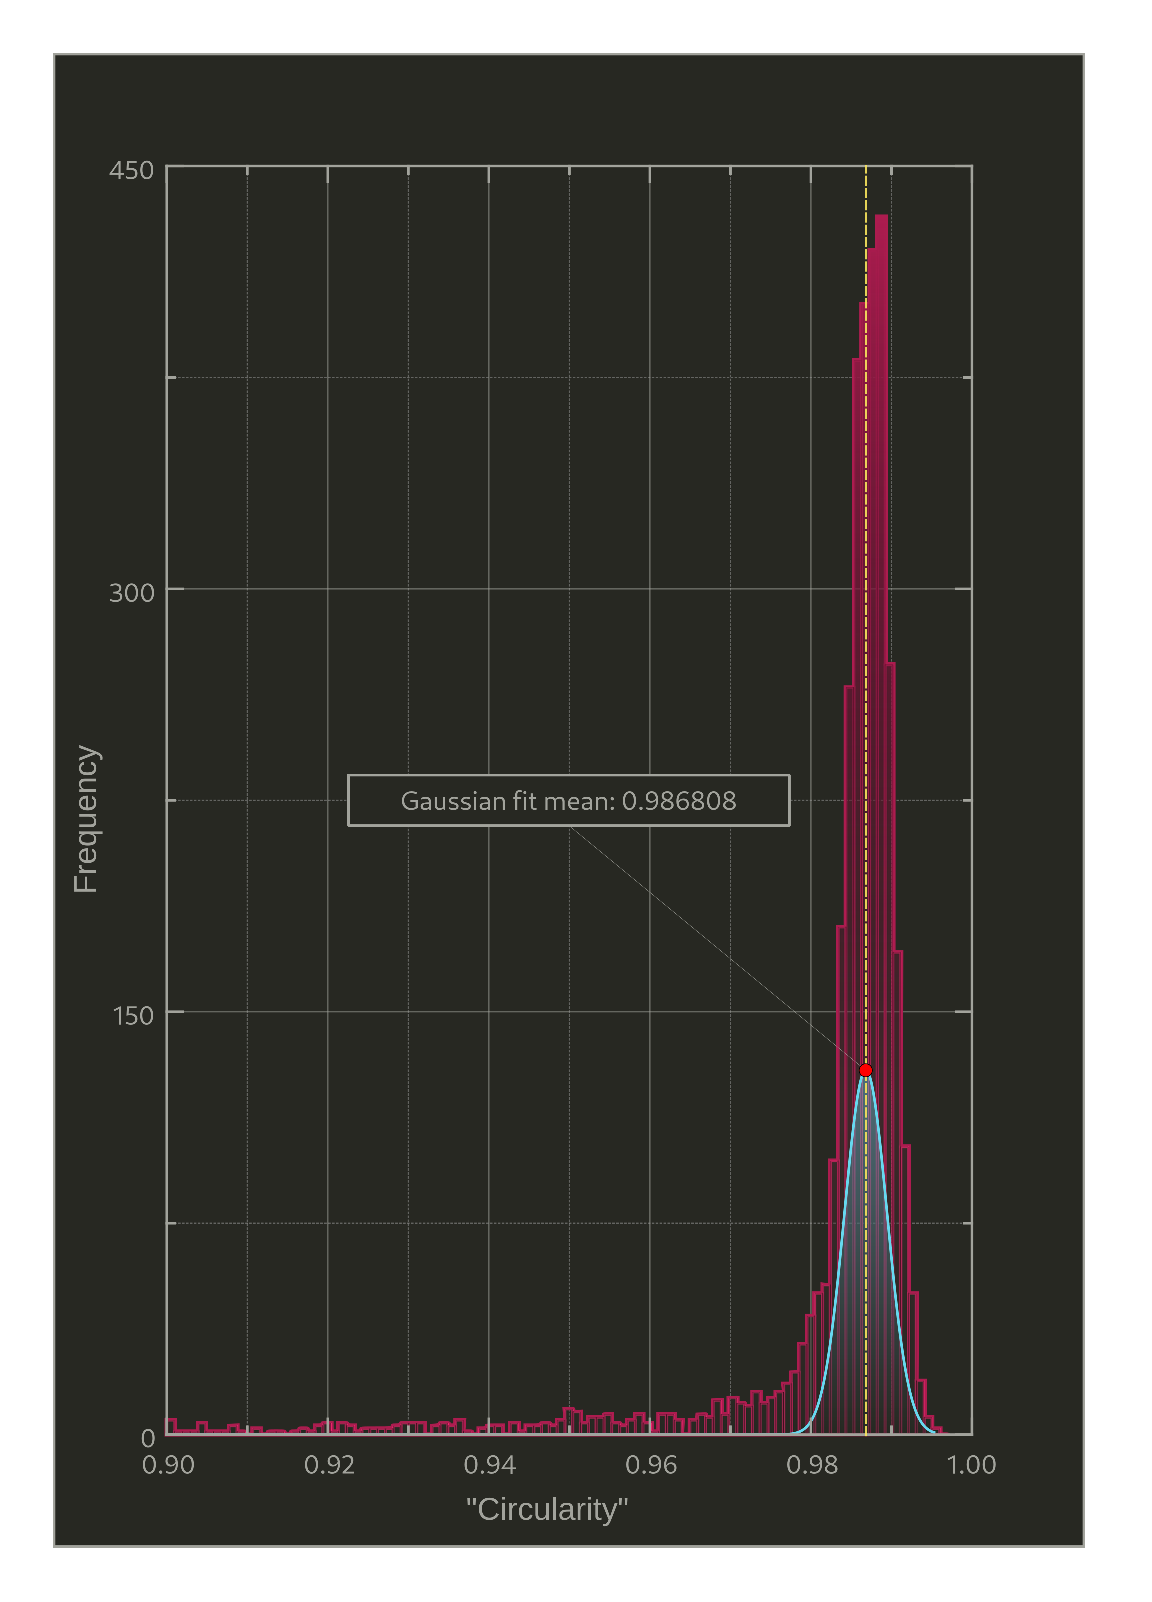
\includegraphics[width=\textwidth]{Pictures/Granulometry_plots/Histogram_Circularity.eps}
            \caption{Particle Circularity Distribution of a powder sample}
            \label{fig:circularity_distribution}
        \end{figure}
  
      \clearpage
  
      The results of the granulometry analysis showcase particle sizes compatible with SLS powder requirements explained in chapter \ref{Powder_requirements}, 
      as well as a great particle circularity distribution, which is consistent with the findings of the 
      SEM analysis reported in section \ref{SEM_analysis_results}. \\
  
      The average particle diameter is 64.4222 $\mu m$, with a count of 144 over a total of more 
      than 3000 analyzed particles, as shown in figure \ref{fig:particle_size_distribution}. \\ 
  
      The average circularity is extremely close to a perfectly spherical shape, with a 
      mean value of roughly 0.98, as clearly visible in figure \ref{fig:circularity_distribution}. \\ 

      \clearpage

    \subsection{DSC Results\label{DSC_results}}

    The analysis results have been analyzed and plotted using \textit{Labplot} \autocites{Labplot} 
    and \textit{Inkscape} \autocites{Inkscape},
    using the \textit{exo-up} convention, with the raw pellet curves used as a baseline for the powder curves. \\
        \begin{figure}[h!]
            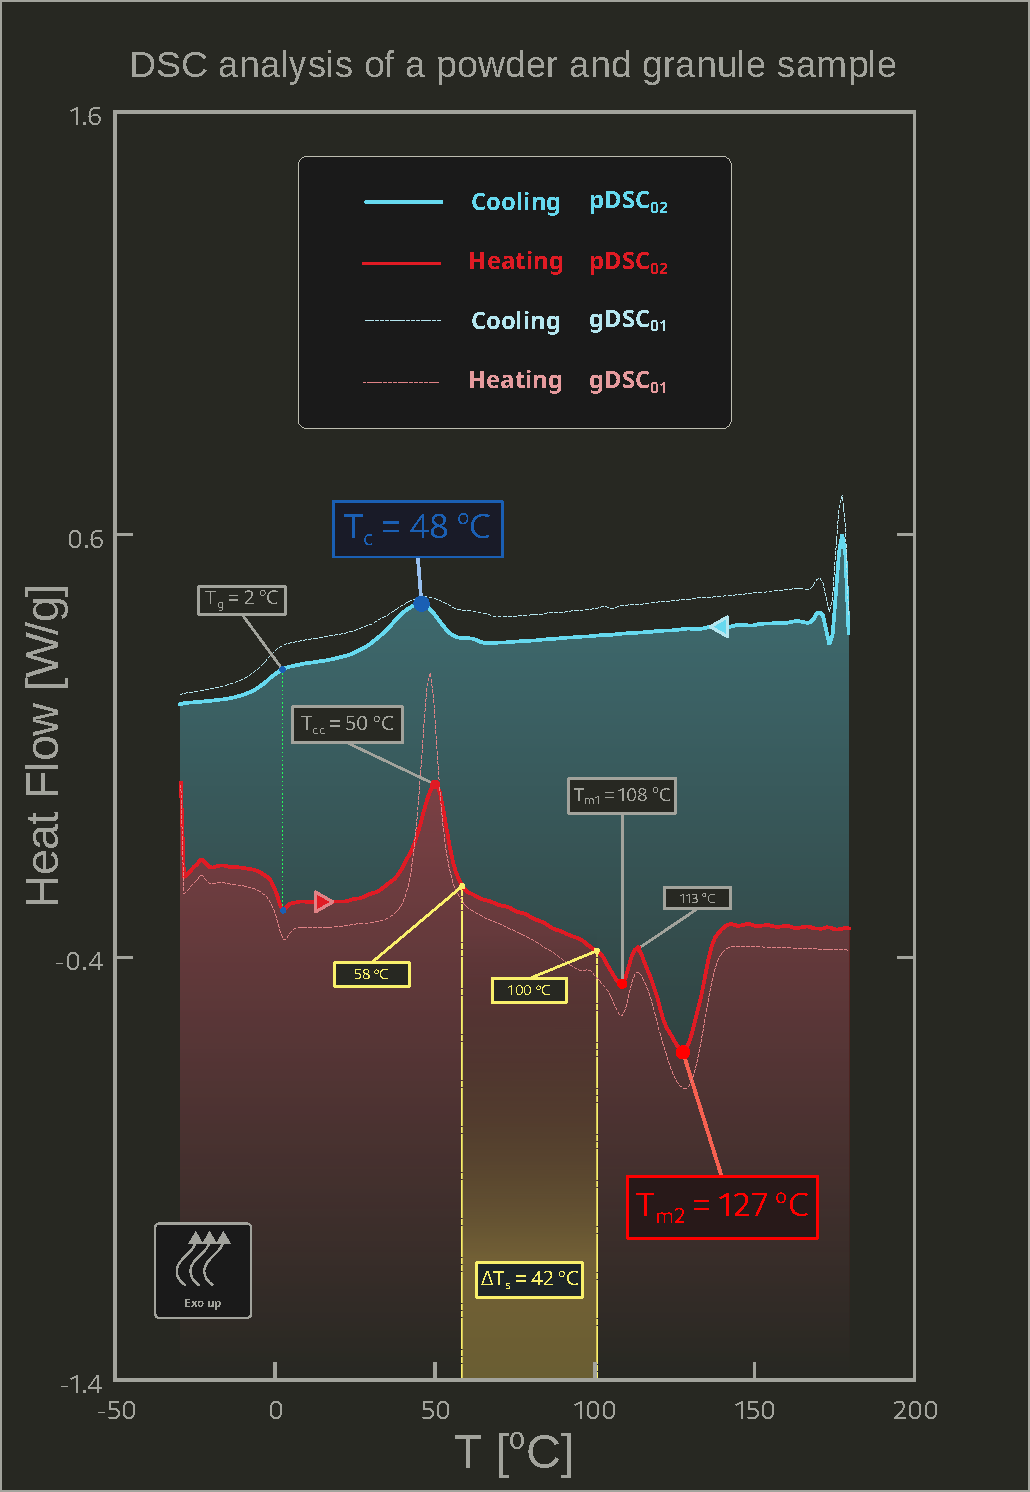
\includegraphics[width=0.9\textwidth]{Pictures/Thermal_analysis_plots/DSC_alberto.pdf}
            \caption{DSC analysis of PHBH at $10 \ ^{\circ}C/min$, exo-up convention}
            \label{fig:DSC_10Cmin}
        \end{figure}

                    %\begin{figure}[h!]
                    %    \centering
                    %    \includegraphics[width=\textwidth]{Pictures/DSC/DSC_01.eps}
                    %    \caption{DSC analysis of powder sample $pDSC_{(10 \ ^{\circ}C/min)}-01$ \autocites{Mettler_Toledo}}
                    %    \label{fig:DSC_01}
                    %\end{figure}
%
                    %\begin{figure}[h!]
                    %    \centering
                    %    \includegraphics[width=\textwidth]{Pictures/DSC/DSC_02.eps}
                    %    \caption{DSC analysis of powder sample $pDSC_{(10 \ ^{\circ}C/min)}-02$ \autocites{Mettler_Toledo}}
                    %    \label{fig:DSC_02}
                    %\end{figure}
%
                    %\begin{figure}[h!]
                    %    \centering
                    %    \includegraphics[width=\textwidth]{Pictures/DSC/DSC_03.eps}
                    %    \caption{DSC analysis of powder sample $pDSC_{(5 \ ^{\circ}C/min)}-03$ \autocites{Mettler_Toledo}}
                    %    \label{fig:DSC_03}
                    %\end{figure}
%
                    %\begin{figure}[h!]
                    %    \centering
                    %    \includegraphics[width=\textwidth]{Pictures/DSC/DSC_04.eps}
                    %    \caption{DSC analysis of sintered sample $sDSC_{(10 \ ^{\circ}C/min)}-04$ \autocites{Mettler_Toledo}}
                    %    \label{fig:DSC_04}
                    %\end{figure}

        \clearpage

        The plot highlights a consistent behaviour  and only 
        minor differences between the powder and pellet samples, with the powder specimen showing a slightly wider 
        sintering window, which is a very desirable trait for SLS, as explained in 
        previous chapters \ref{Powder_requirements}, \ref{PHBH} and in accordance with 
        the available literature \autocites{Eraslan_PHBH_review,doi:10.1063/1.4918516,DechetMaximilianA2020OtDo}. \\    
        
        As evident from the heating phase (visible in figure \ref{fig:DSC_10Cmin}), the powder sample shows a main peak melting point of $T_{m} =  127.164 \ ^{\circ}C$, with 
        a secondary melting point of $T_{m} =  108.164 \ ^{\circ}C$, as well as a crystallization point at $T_{c} =  50.1643 \ ^{\circ}C$. 

        The cooling phase highlights a main peak crystallization point of $T_{c} =  48.254 \ ^{\circ}C$ as well, indicating 
        that the main crystallization activity occurs around that temperature range in both phases. \\ 

        A minor peak activity is also observed at around $2 \ ^{\circ}C$ in both the heating and cooling phases
        (with a more prominent peak during heating), and this can be attributed to the
        glass transition temperature of the polymer, which can be further investigated using a DMA, as documented in section \ref{DMA}. \\

        The powder sample data has been used to calculate the enthalpy values around the two main crystallization peaks and the main 
        melting peak, with the following approach: \\

        \begin{itemize}
            \item The heat flow data points are normalized by the specimen weight, which does not have a data set of its own from the DSC test, 
            but can be assumed to be constant within the temperature range, which is a resonable 
            assumption based on the TGA results (explored in detail in chapter \ref{TGA_Results}).
            \item The normalized heat flow is then plotted against time for both the heating and cooling phases and 
            a line is hand drawn around the peaks
            \item The area between the peaks and the base line represents an estimate of the enthalpy value  
        \end{itemize}

        The enthalpy values are then calculated using the following equation, which is solved numerically: \\ 

        \begin{equation}
            \Delta H = \int_{t_0}^{t_1} \phi (t) \,dt \ \ \ \ [J/g]
            \label{eq:enthalpy}
        \end{equation}

        where $\phi (t)$ is the normalized heat flow and $t_0$ and $t_1$ are the time values at which the line is drawn. 

        \clearpage

        \begin{figure}[h!]
            \centering
            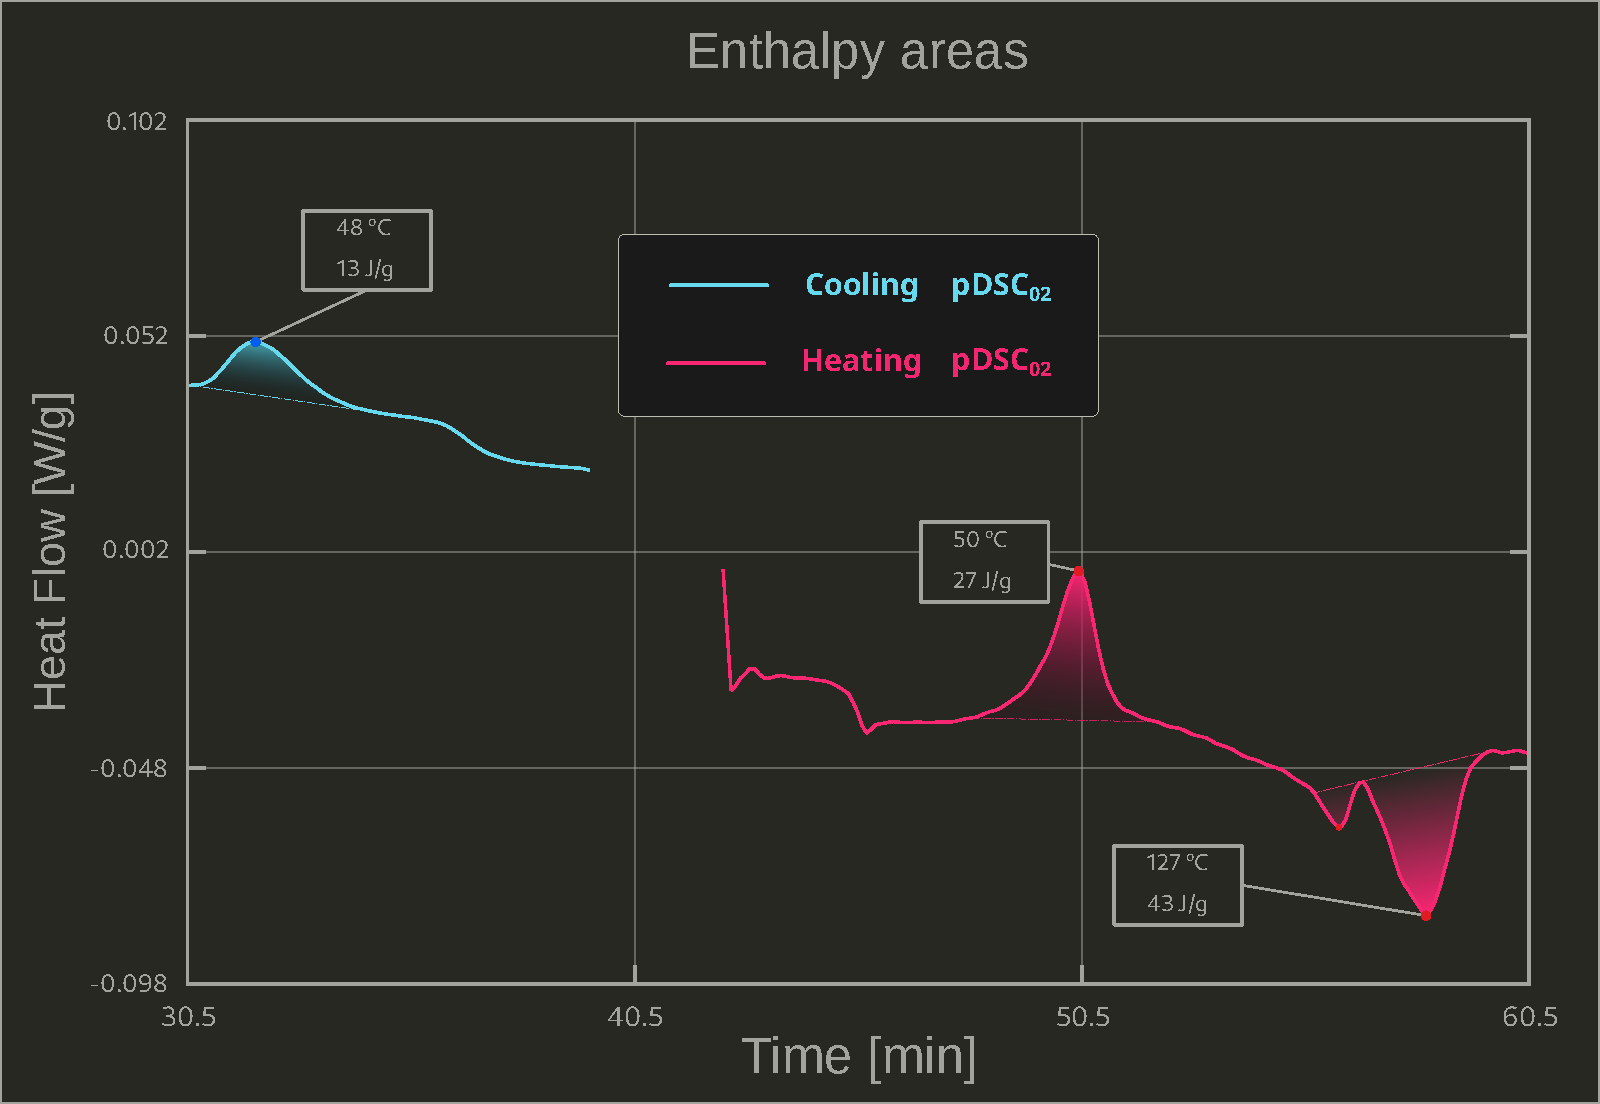
\includegraphics[width=\textwidth]{Pictures/Thermal_analysis_plots/DSC_peaks_areas.pdf}
            \caption{Enthalpy values for the DSC analysis of PHBH at $10 \ ^{\circ}C/min$}
            \label{fig:DSC_enthalpy}
        \end{figure}

        The obtained enthalpy values can be used to derive the estimated percentage of crystallinity of the material, using the following equation: \\

        \begin{equation}
            X_c = \frac{\Delta H_{m} - \Delta H_{cc}}{\Delta H_{m}^{0} \cdot m} \ \ \ \ [\%]
            \label{eq:crystallinity}
        \end{equation}

        where $\Delta H_{m}$ is the enthalpy value of the melting peak, $\Delta H_{cc}$ is the enthalpy value of the cold crystallization peak, 
        m is the mass of the specimen and $\Delta H_{m}^{0}$ is the enthalpy value of the melting peak of a pure crystalline material, 
        which is $146 \ J/g$ for PHBH \autocites{PHBH_Crystallinity}. \\

        All the highlighted temperatures and other relevant quantities are summarized in the following table: 

                \begin{table}[h!]
                    \resizebox{\textwidth}{!}{%
                        \begin{tabular}{@{}cccccccccccc@{}}
                        \toprule
                        \textit{\textbf{ID}} & \textit{$\Delta H_c \ [J/g]$} & \textit{$T_{c}^{p} \ [^{\circ}C]$} & \textit{$T_g \ [^{\circ}C]$} & \textit{$T_{cc}^{p} \ [^{\circ}C]$} & \textit{$\Delta H_{cc} \ [J/g]$} & \textit{$\Delta H_m \ [J/g]$} & \textit{$T_{m1}^{o} \ [^{\circ}C]$} & \textit{$T_{m1}^{p} \ [^{\circ}C]$} & \textit{$T_{m2}^{o} \ [^{\circ}C]$} & \textit{$T_{m2}^{p} \ [^{\circ}C]$} & \textit{$X_c \ [\%]$} \\ \midrule
                        gDSC                 & 11                            & 49                                    & 2                            & 49                                     & 36                               & 49                            & 103                                     & 108                                & 111                                         & 129                                    & 11                    \\
                        pDSC                 & 13                            & 48                                    & 2                            & 50                                     & 27                               & 43                            & 100                                     & 108                                & 113                                         & 127                                    & 15                    \\ \bottomrule
                        \end{tabular}%
                    }
                    \caption{Results of the DSC analysis showcasing phase transition points, enthalpies and crystallinity of the material}
                    \label{tab:DSC_Results}
                \end{table}

        \clearpage

        \subsection{TGA Results\label{TGA_Results}}
        The analysis data has been exported with \textit{Mettler-Toledo}'s included software \autocites{Mettler_Toledo}, after normalizing the data to the initial weight of the sample,
        then imported, elaborated and plotted with \textit{Labplot} \autocites{Labplot}. \\
        The following figures show the results of the TGA analysis on the pellet, powder and sintered samples. \\ 
        \begin{figure}[h!]
            \centering
            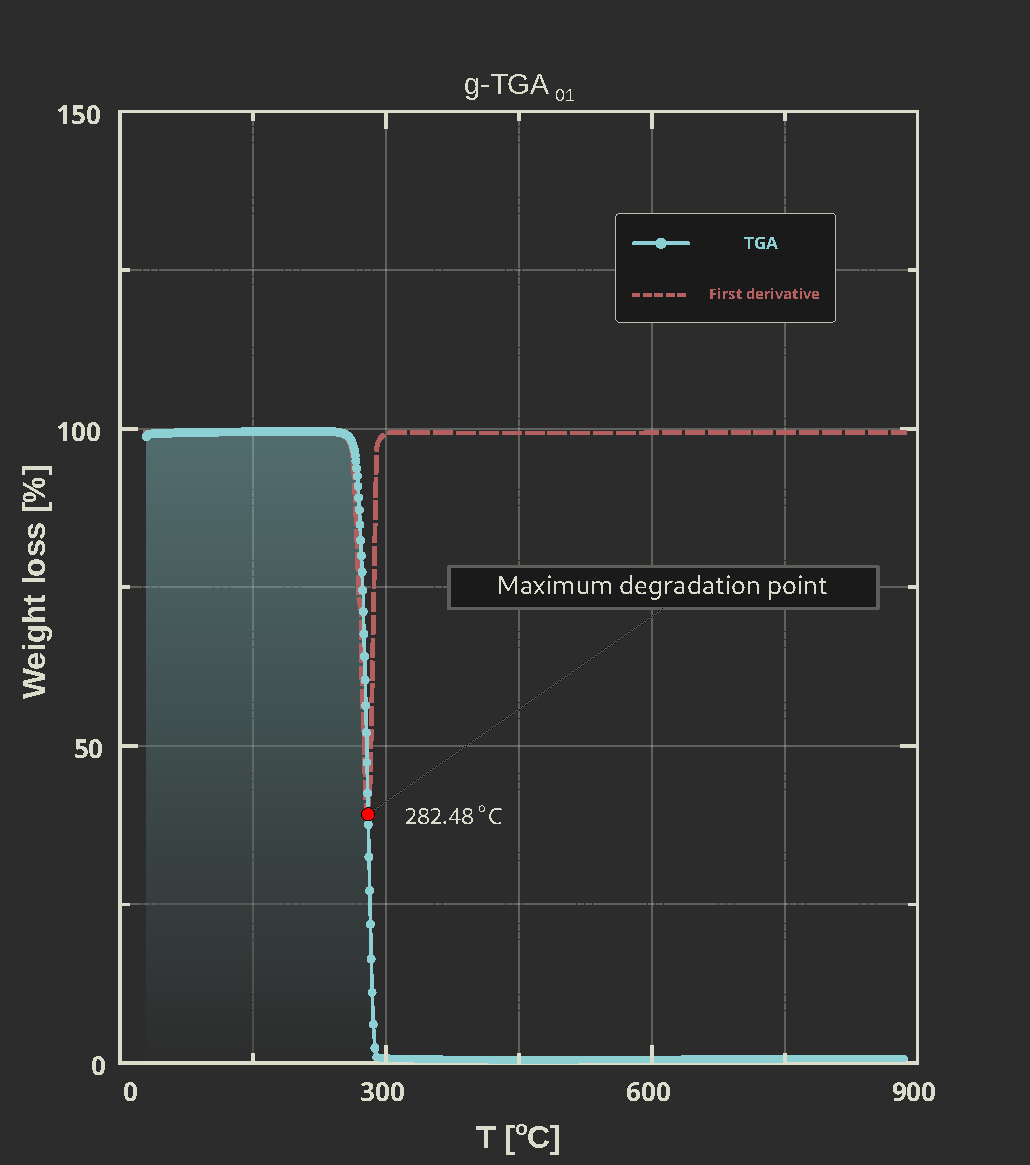
\includegraphics[width=0.8\textwidth]{Pictures/Thermal_analysis_plots/TGA_catalogued/Fixed/g-TGA01.pdf}
            \caption{TGA analysis of pellet sample $gTGA_{01}$ (as in table \ref{tab:TGA_specimens})}
            \label{fig:TGA_01}
        \end{figure}
        \begin{figure}[h!]
            \centering
            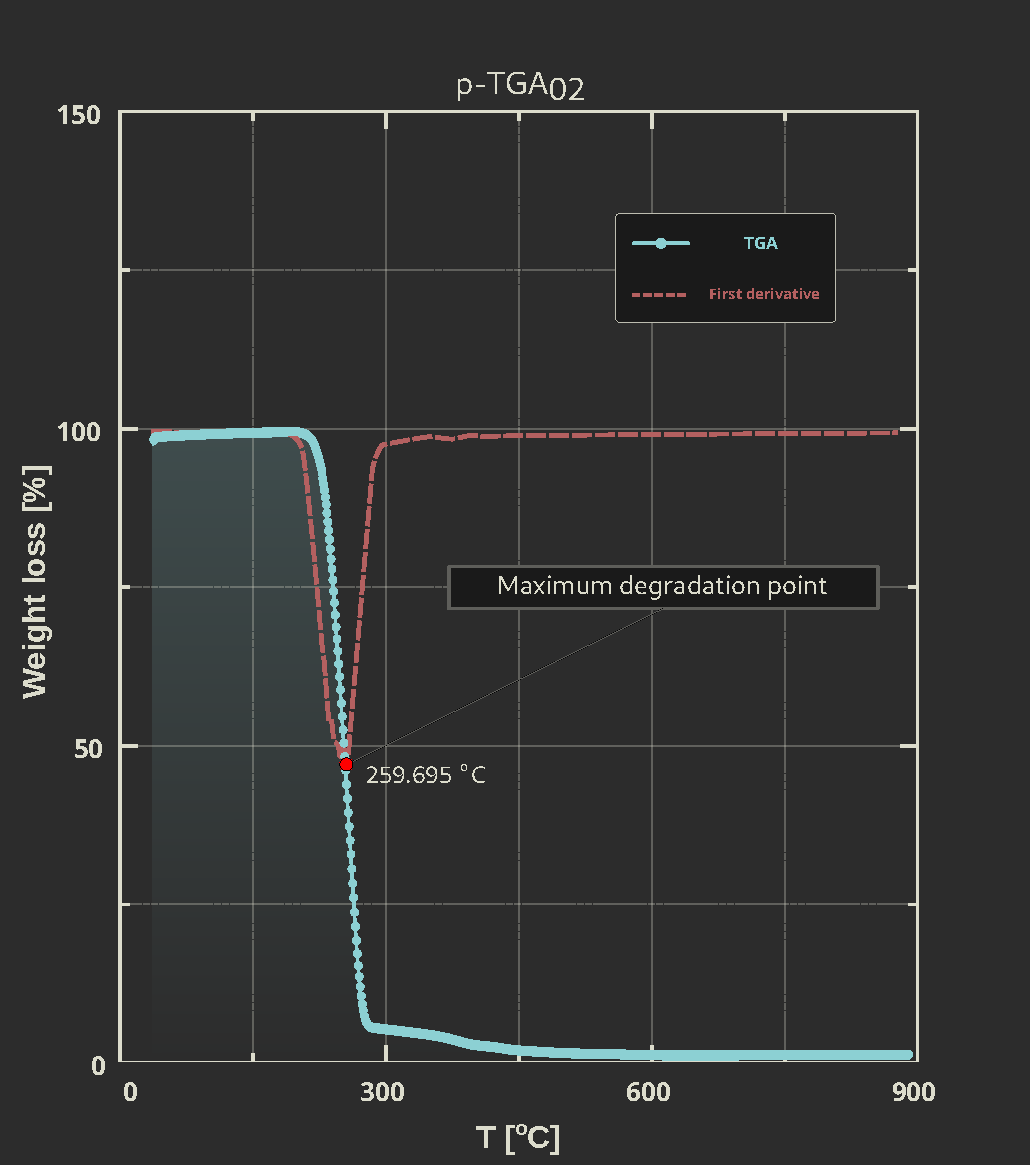
\includegraphics[width=0.8\textwidth]{Pictures/Thermal_analysis_plots/TGA_catalogued/Fixed/p-TGA02.pdf}
            \caption{TGA analysis of powder sample $pTGA_{02}$ (as in table \ref{tab:TGA_specimens})}
            \label{fig:TGA_02}
        \end{figure}
        \begin{figure}[h!]
            \centering
            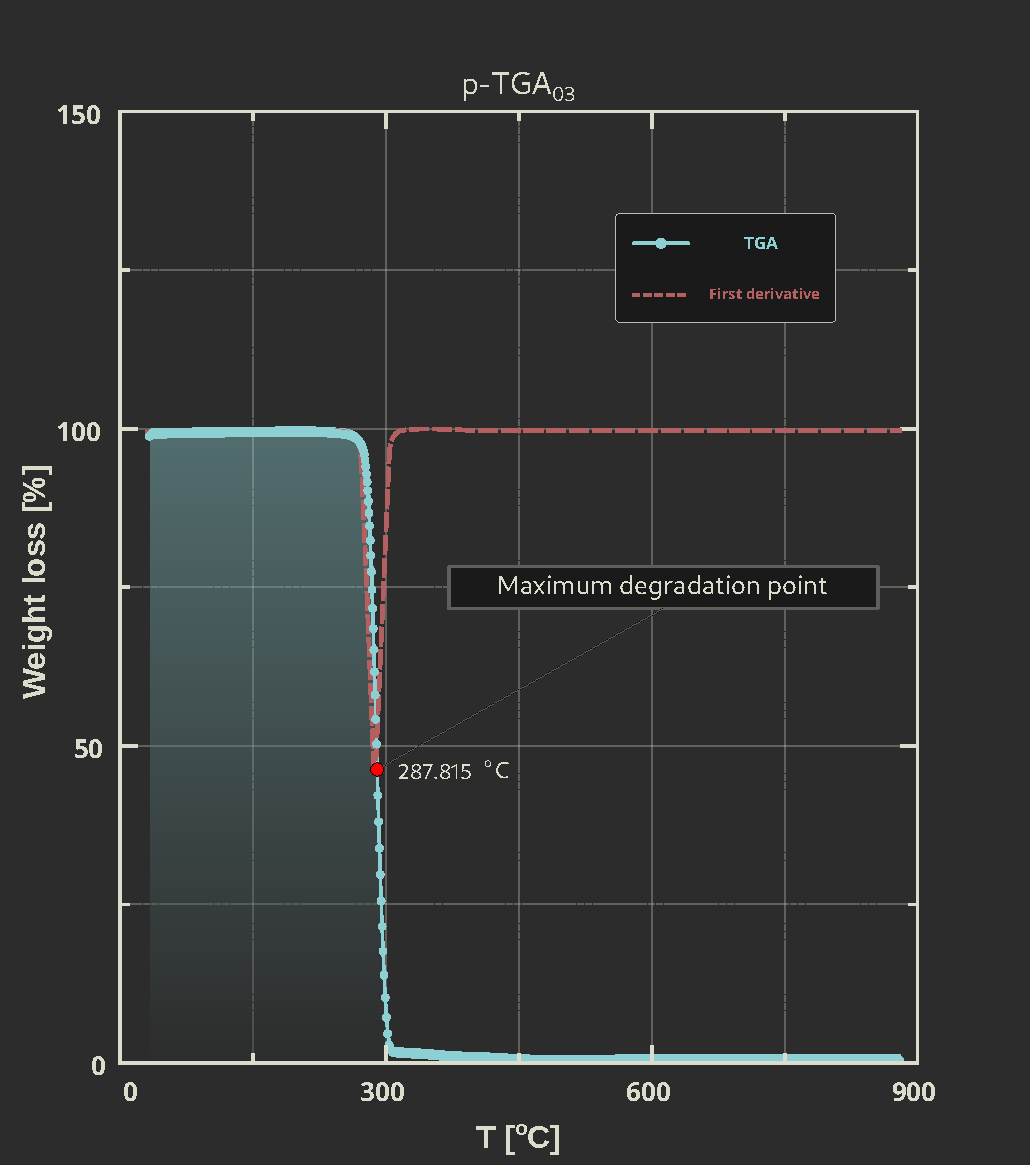
\includegraphics[width=0.8\textwidth]{Pictures/Thermal_analysis_plots/TGA_catalogued/Fixed/p-TGA03.pdf}
            \caption{TGA analysis of powder sample $pTGA_{03}$ (as in table \ref{tab:TGA_specimens})}
            \label{fig:TGA_03}
        \end{figure}

            \begin{figure}[h!]
                \centering
                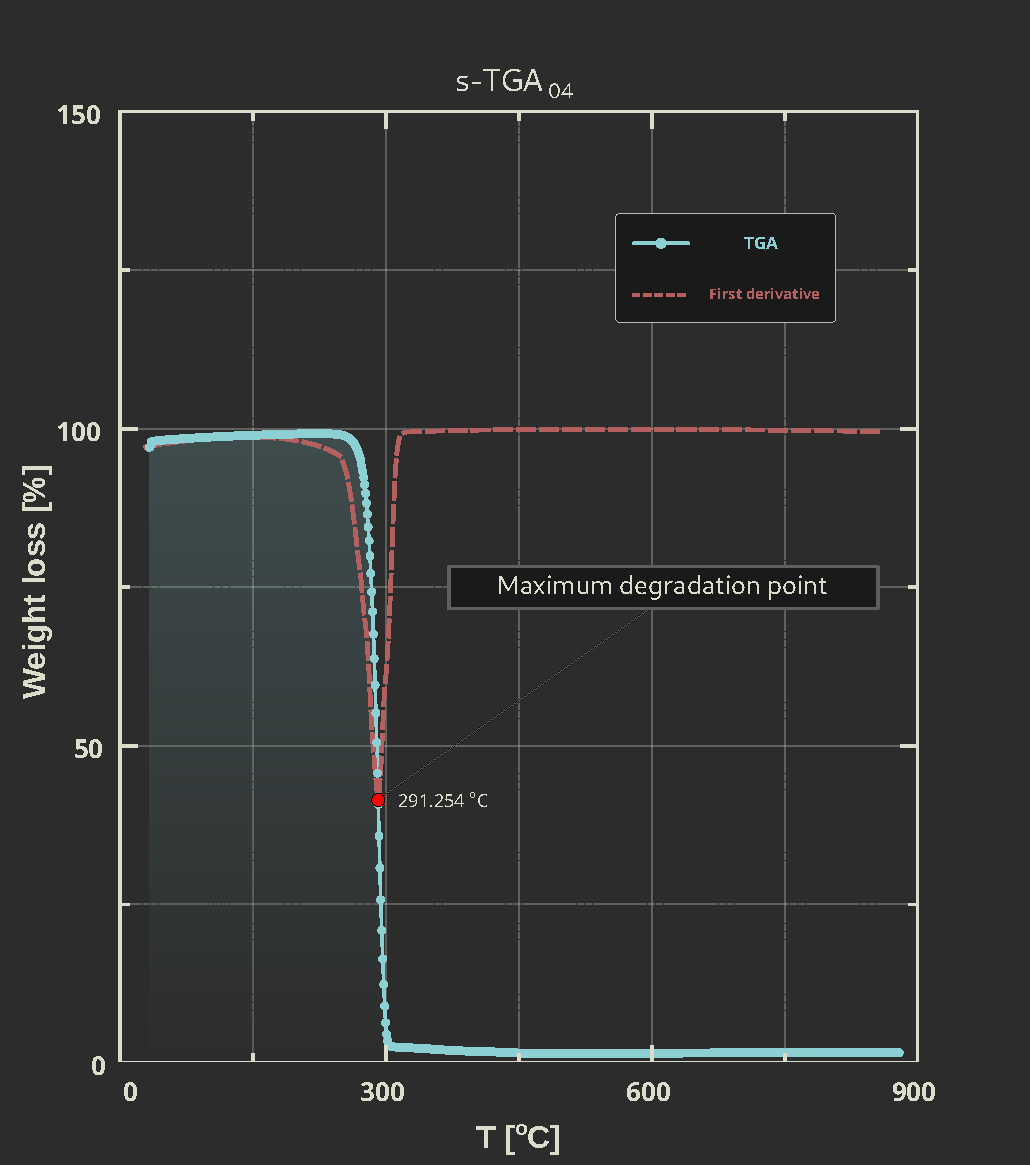
\includegraphics[width=0.8\textwidth]{Pictures/Thermal_analysis_plots/TGA_catalogued/Fixed/s-TGA04.pdf}
                \caption{TGA analysis of sintered sample $sTGA_{04}$ (as in table \ref{tab:TGA_specimens})}
                \label{fig:TGA_04}
            \end{figure}

            \clearpage

            The results of the TGA analysis showcase the expected thermal behaviour of the powder and sintered samples,
            which are consistent with the pellet sample. \\ 

            The TGA curves show an exponentially incresing weight loss, with very similar slopes, and the additional 
            first derivative showcases a consistent behaviour among all samples, with clear degradation peaks at approximately 
            the same temperature values. \\ 

            As a further testimony of the consistent thermal behaviour of the biopolymer along the entire pipeline, the overlap of the
            TGA curves of the pellet, powder and sintered samples is shown in the following figure:

                \begin{figure}[h!]
                    \centering
                    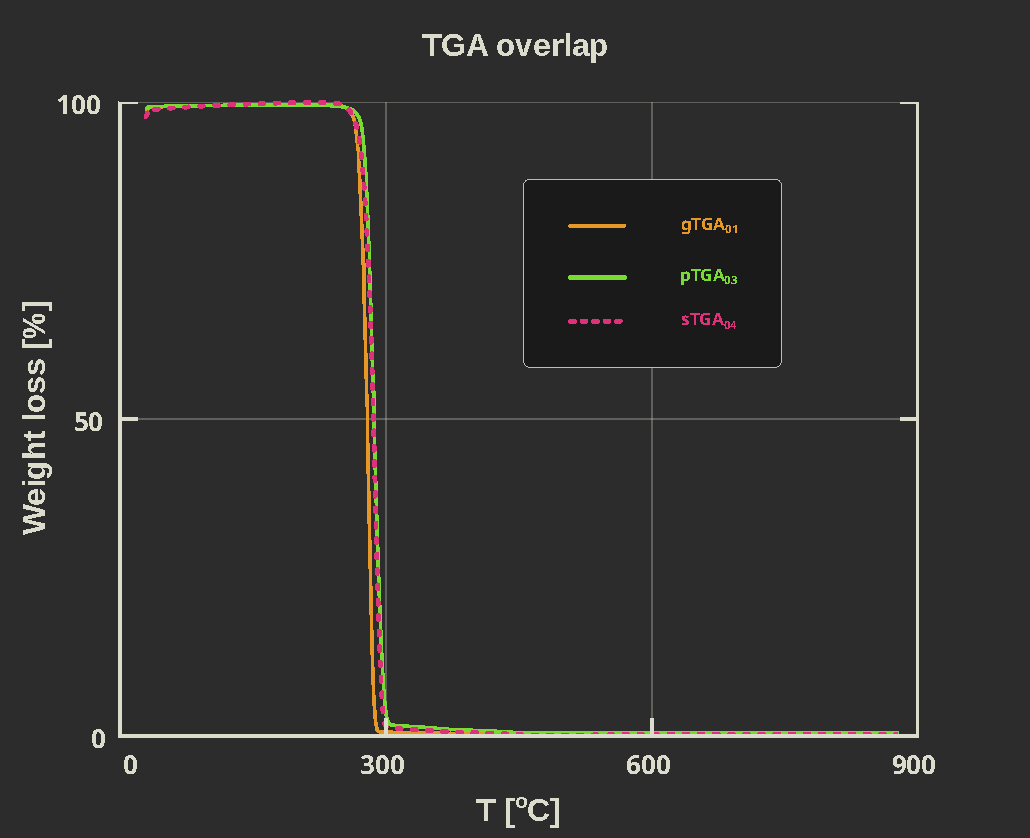
\includegraphics[width=\textwidth]{Pictures/Thermal_analysis_plots/TGA_catalogued/Fixed/TGA_overlapped.pdf}
                    \caption{Consistent results of the TGA analysis of the pellet, powder and sintered samples}
                    \label{fig:TGA_overlapped}
                \end{figure}

        \clearpage

        \subsection{DMA Results\label{DMA_Results}}

        The results of the DMA analysis are shown in the following figure, where the tan$\delta$ curve has been upscaled significantly 
        in order to match a relative scale with the other curves. \\ 

            \begin{figure}[h!]
                \centering
                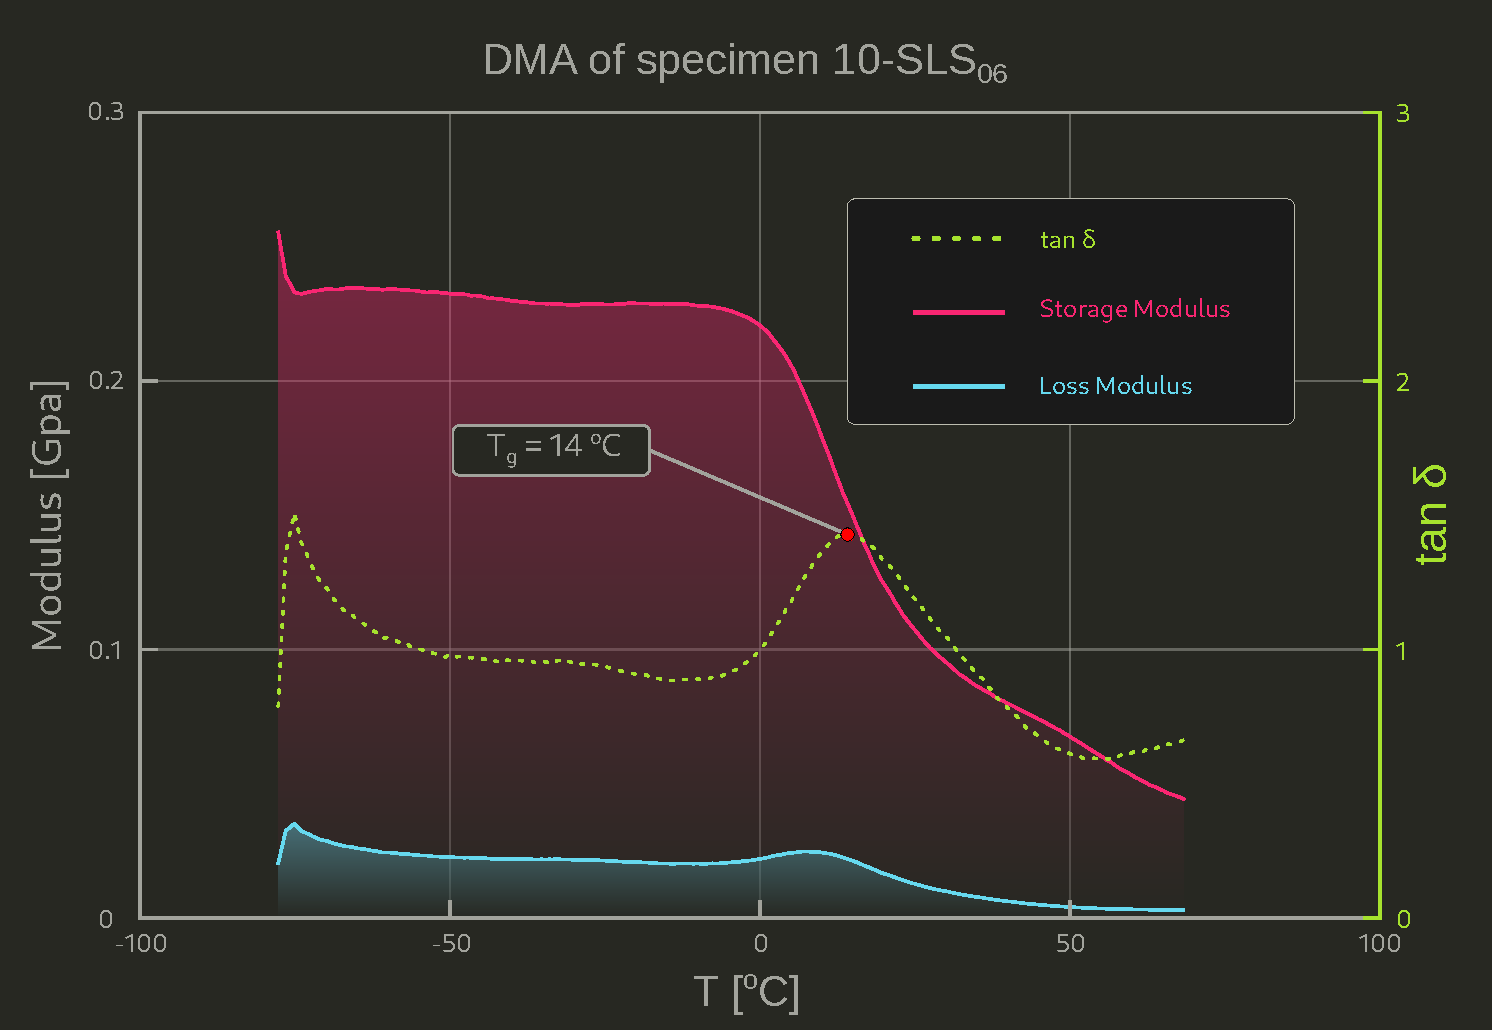
\includegraphics[width=\textwidth]{Pictures/Thermal_analysis_plots/DMA.pdf}
                \caption{DMA analysis of sample $10-SLS_{06}$ (as reported in table \ref{tab:SLS_samples}).}
                \label{fig:DMA_plot}
            \end{figure}

        \clearpage 

        The tan$\delta$ curve visible in figure \ref{fig:DMA_plot} shows a clear peak at $14.1 \ ^{\circ}C$, which is the glass transition temperature of the material, 
        in disaccordance with the initial estimation of $2 \ ^{\circ}C$ (\ref{fig:DSC_10Cmin}). \\ 

        As expected for a polymer of the PHA family, both the storage modulus $E'$ and the loss modulus $E''$ are very low, in line with the 
        typical viscoelastic behavior of all bio-based polymers \autocites{Kovalcik_PHA_Review}, which are not suited for structural applications and 
        are instead used for packaging and other non-structural applications, such as biomedical implants and scaffolds \autocites{Messori_Bondioli_PHAs}. \\

        Unsurprisingly, the mechanical properties of the material fall behind those of typical SLS polymers, which can 
        occasionally reach storage moduli a whole order of magnitude higher than that of PHBH, according to this DMA. \\ 

        That in itself is not a major issue, as SLS parts are not limited to structural applications or mechanical pieces:
        other properties, such as biodegradability, biocompatibility and low toxicity can be very desirable traits in a wide range of 
        applications. \\ 

        Moreover, the mechanical and thermal properties of the material can be improved by adding fillers, creating blends with other 
        bio-based polymers or creating composites with other materials. \\ 

        Given the successful SLS printability, with unaltered thermal properties among the raw material, the powder and the 
        printed parts (as highlighted by the TGA and DSC analysis results \ref{TGA_Analysis}, \ref{DSC_analysis}), as well as 
        mechanical properties that meet the expected behavior of a bioplastic, PHBH is a very promising polymer 
        that can further enrich the catalogue of sustainable materials available for additive manufacturing. \\ 



    \clearpage
    \section{3D printing\label{SLS_printing_experimental}}

    After the powder has been characterized, the next step is to print it with the SLS machine. \\

    Before being printed, the powder can be mixed with a small quantity of a binder, to improve the flowability of the powder. 
    However, given the excellent flowability of the PHBH powder (highlighted in section \ref{flowability_analysis}), this step has been skipped. \\

    The next preparation step is to further dry the powder, in order to remove any residual moisture
    that could have accumulated during the storage period, and to homogenize the powder distribution 
    by shaking the container for a few minutes. \\

                \begin{figure}[h!]
                    \centering
                    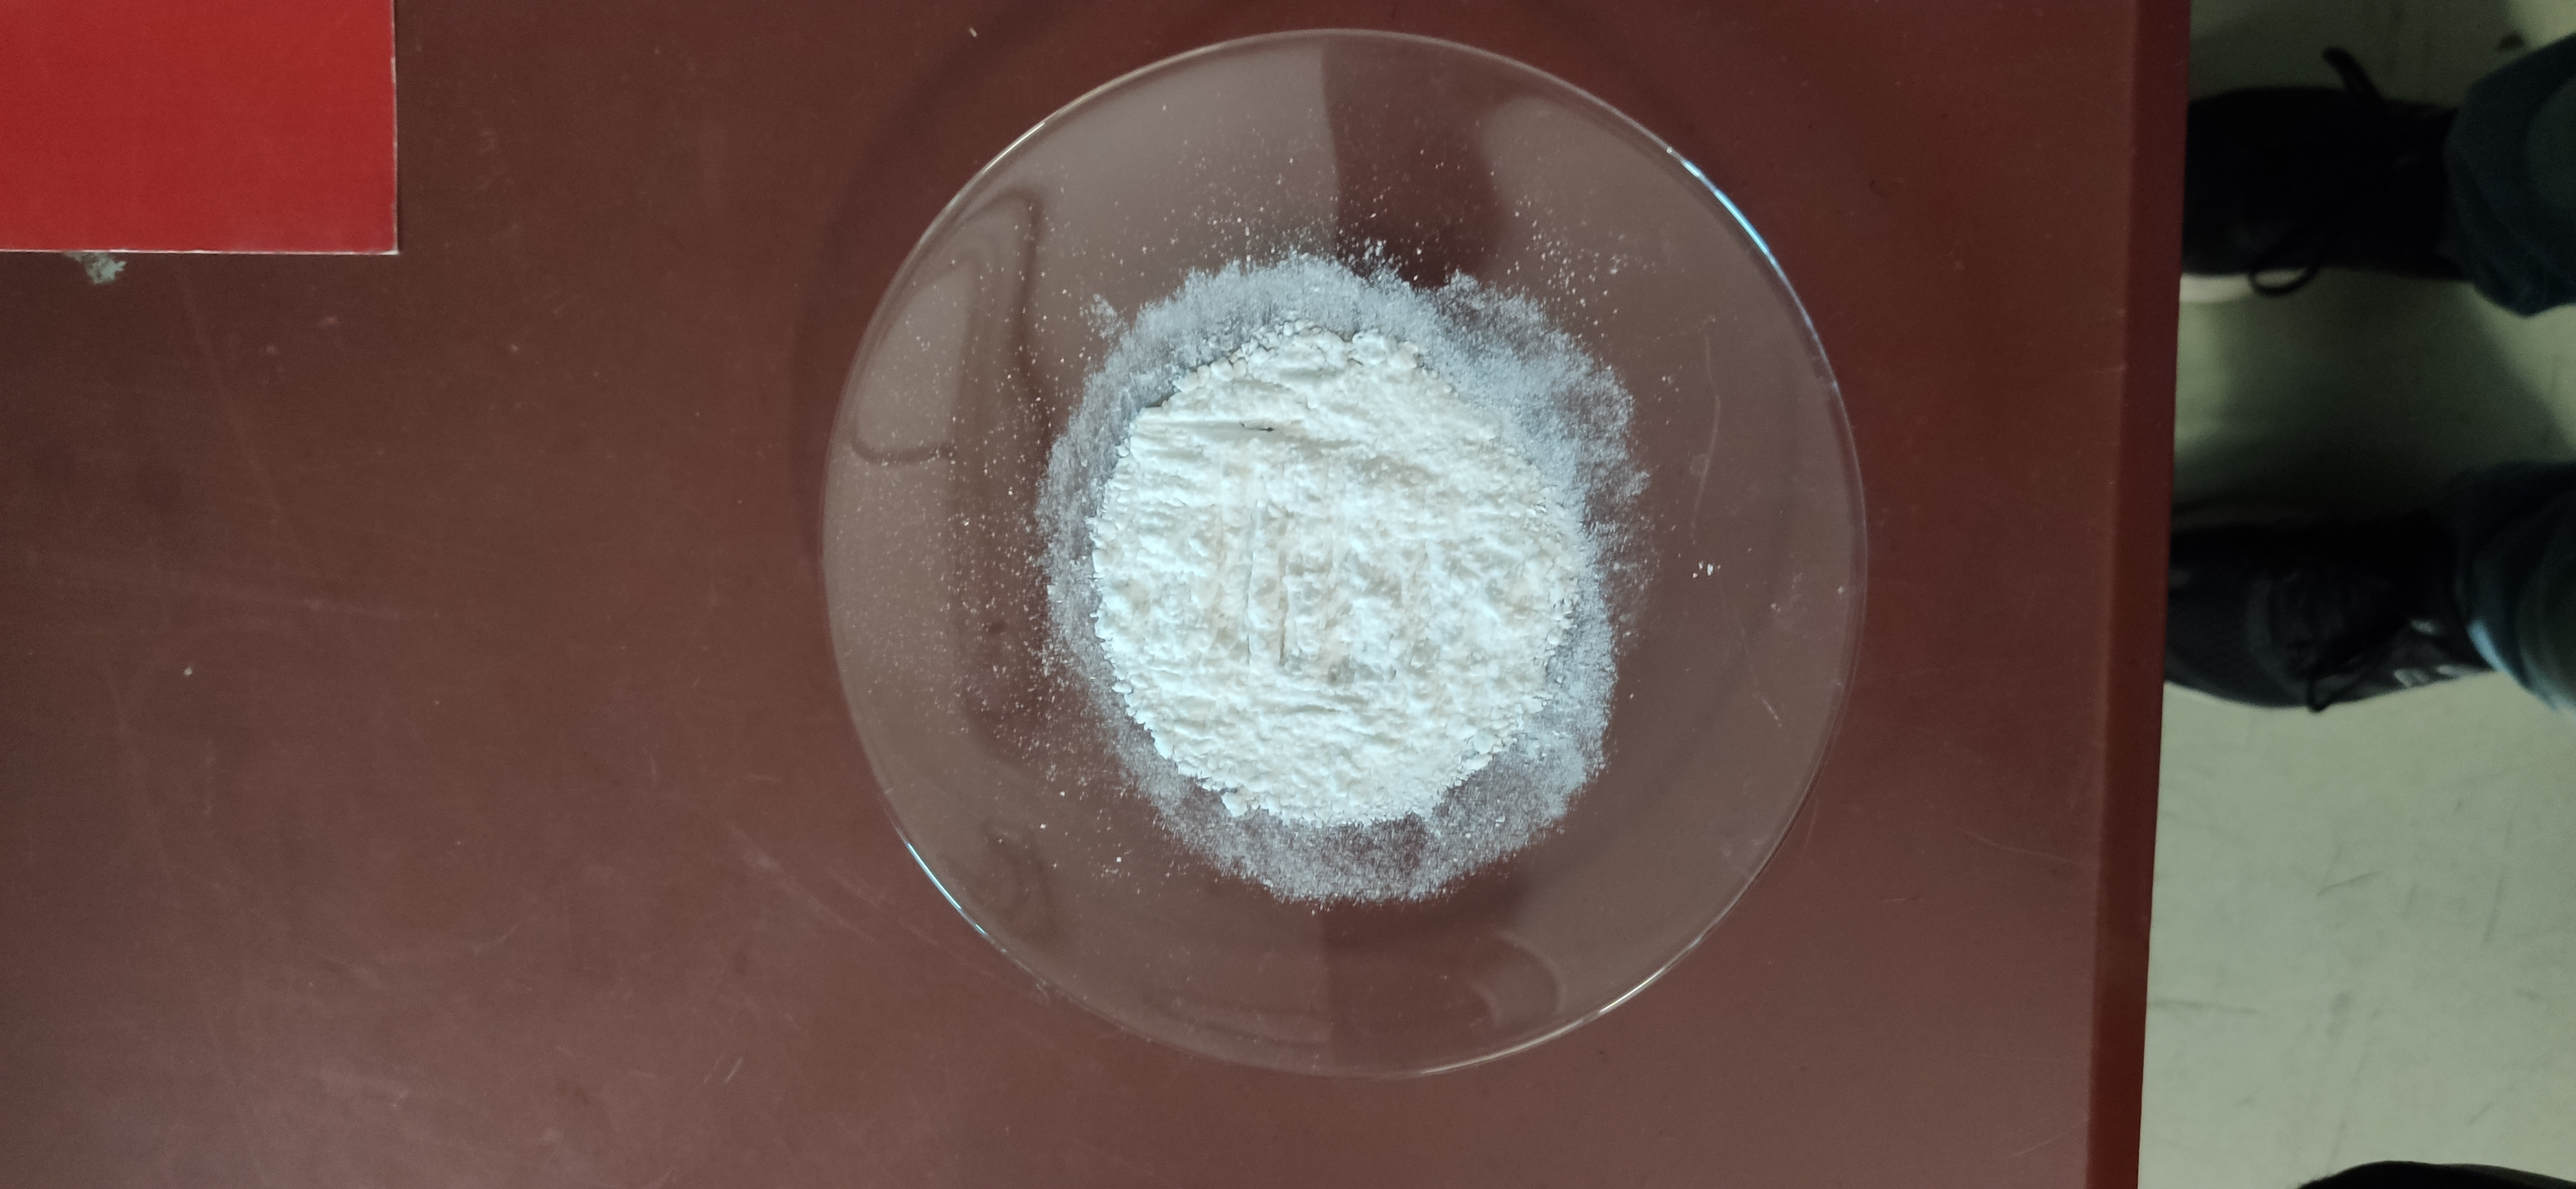
\includegraphics[width=0.5\textwidth]{Pictures/PHBH_dried_powder.eps}
                    \caption{SLS ready powder batch}
                    \label{fig:PHBH_collected_powder}
                    
                \end{figure}

        \subsection{Print files preparation\label{Print_files_preparation}}

        The next step is to prepare the print files, which are the files that will be sent to the SLS machine, 
        to instruct it on how to print the part. \\

        The approach can vary depending on the software used to prepare the files, but the general idea is to 
        create a 3D model of the part, then slice it into layers, and finally export the files to the SLS machine. \\

        The pipeline starts with the creation of a 3D model of the part and ends with a g-code file, and can 
        be summarized as follows: 
        
                \begin{figure}[h!]
                    \centering 
                    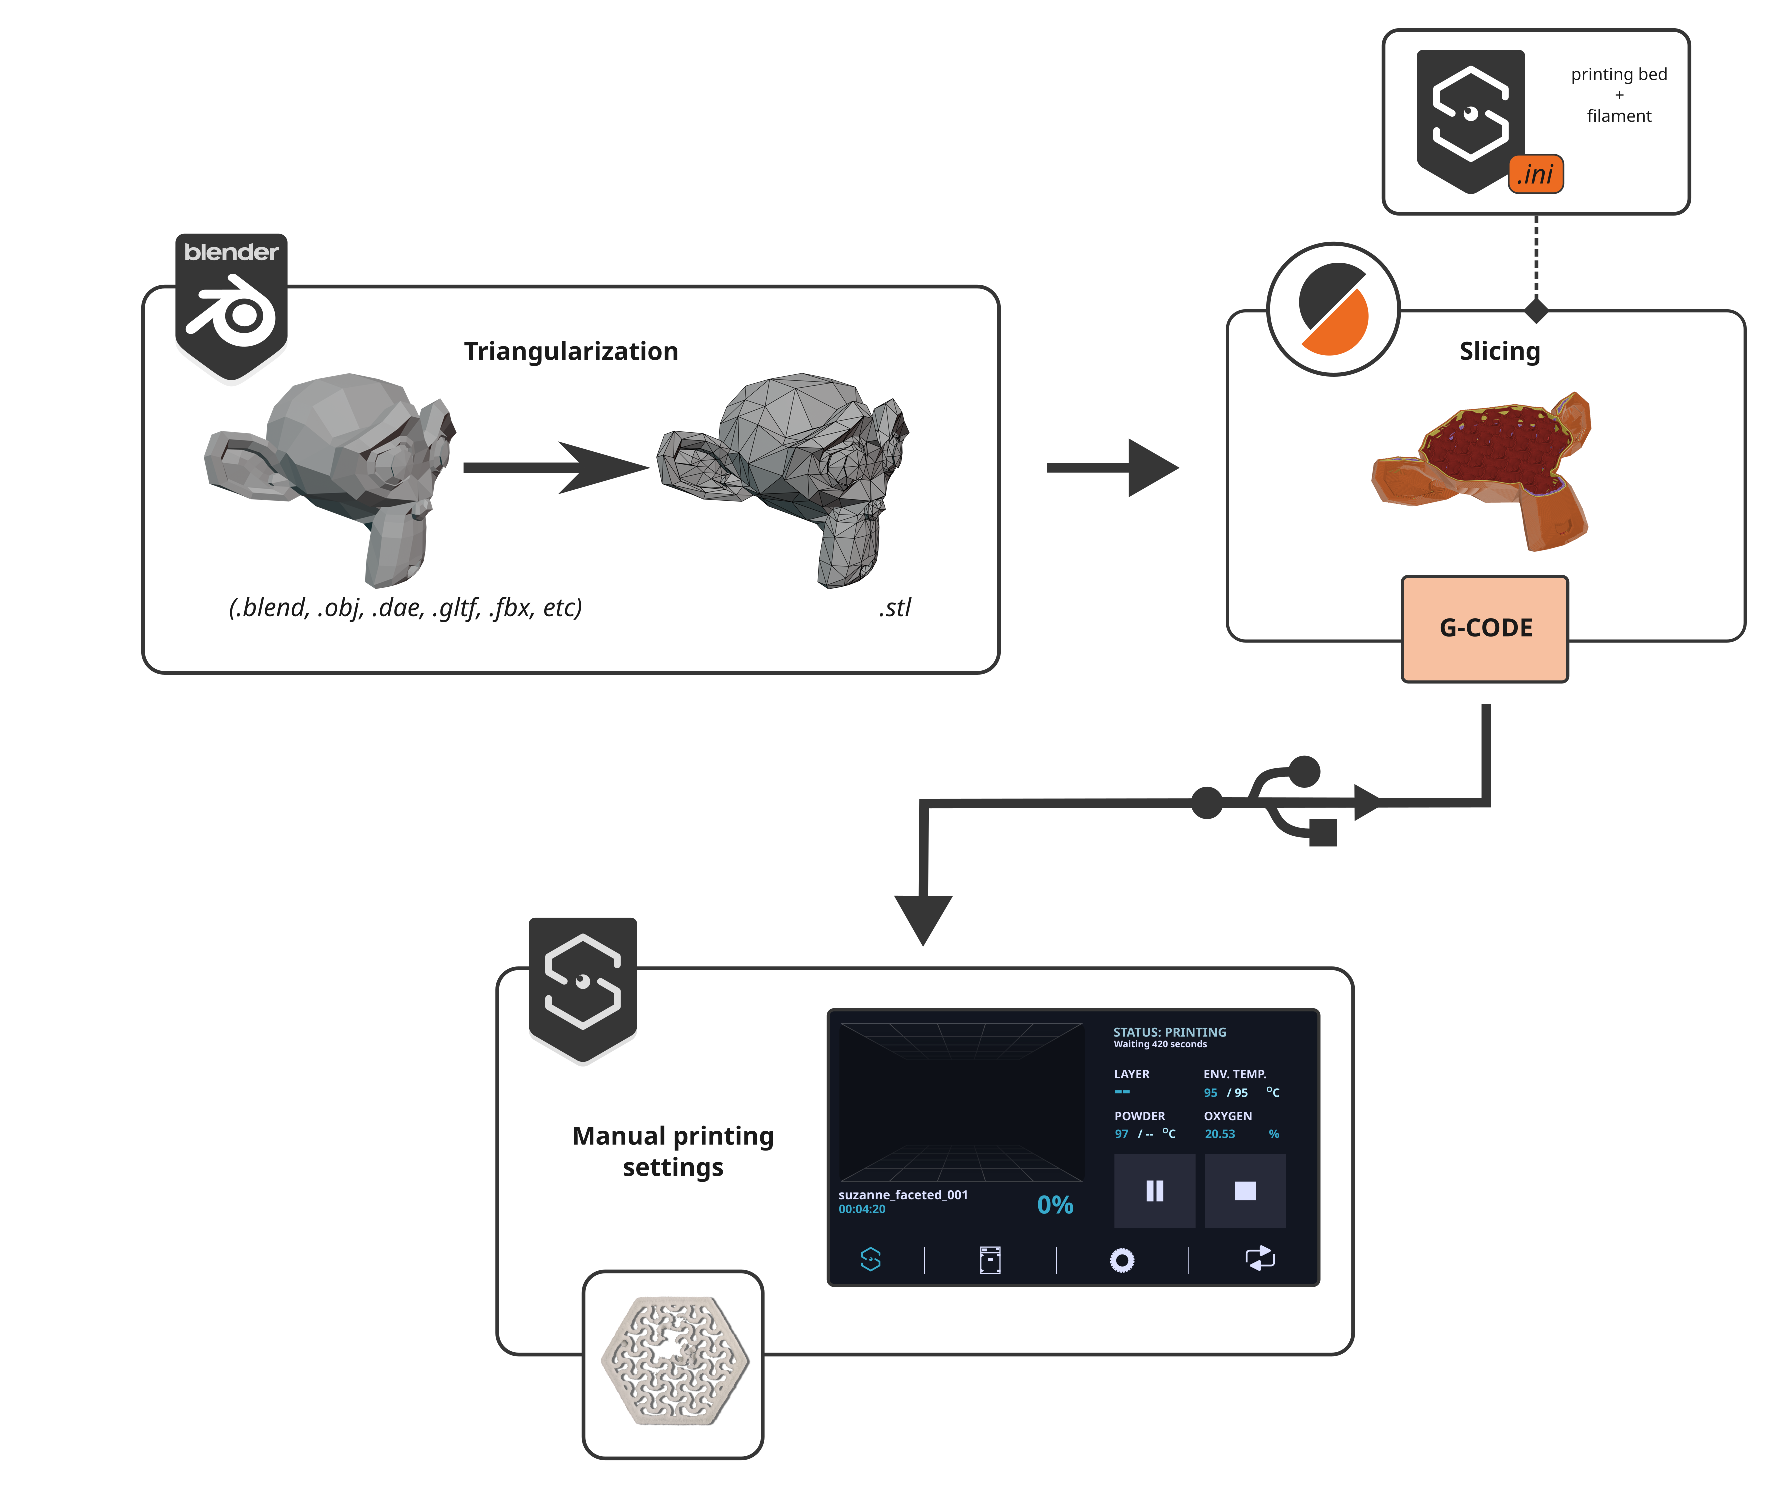
\includegraphics[width=\textwidth]{Pictures/3dprint_file_pipeline_scheme.eps}
                    \caption{3D printing file pipeline}
                    \label{fig:3dprint_file_pipeline_scheme}
                \end{figure}

        \subsubsection{3D model creation\label{3D_model_creation}}

        The first step is to create a 3D model of the part, which can be done in many ways, 
        depending on the software used. \\

        The models have been created from scratch, either by directly modeling them in \textit{Blender} 3.3.1 \autocites{Blender},
        or by creating SVG files in \textit{Inkscape} 1.2 \autocites{Inkscape} and then extruding them in \textit{Blender}, where
        they are handled as bezier curves. \\

        This approach is particularly useful for this case study, where planar complex geometries better suit the SLS printing process
        with low powder availability and low printing volumes. As seen in \ref{Printed_samples}, the SLS printed parts 
        are extremely small, with heights in the order of millimeters. \\
        
        Working with planar geometries also allows to easily create very intricate 3D models, by simply extruding the 2D SVG file, 
        which as earlier mentioned is handled as bezier curves and inherits their properties, such as resolution 
        dependant smoothness, non destructive extrusion and custom profile beveling. \\

        The extruded bezier curves have then been converted to meshes, remeshed when necessary, and finally 
        exported as STL files (which is the most common file format for 3D printing), using 
        Blender's internal 3D Printing Toolbox addon, which also offers useful mesh stats and 
        automatic mesh fixing tools. \\
        
        \subsubsection{Slicing\label{Slicing}}
        
        The next step is to slice the 3D model into layers, which is done by the slicing software. \\

        The slicing software takes the STL file as input (or other formats such as OBJ, which are
        automatically triangulated during the import), and outputs a g-code file, which is the file that will be sent to the SLS machine. \\

        There are some caveats with slicing software, which are worth mentioning. \\

        The first one is that the software is not able to handle meshes with non manifold edges, so 
        the STL file must be checked for non manifold edges before being imported. \\ 

        More importantly, all slicing software is designed to work with an FDM workflow, whereas 
        many industrial SLS machines tend to have a dedicated CNC software. 

        This means that the slicing software is not able to handle the SLS workflow without workarounds. 

        The most common workaround is to load a custom configuration file for the slicing software, 
        which will instruct it on how to handle the SLS workflow for a specific printer. 
        The slicing software is not aware of the SLS workflow, so it will slice the model 
        based on a FDM workflow, and the custom configuration file, which bundles a set of 
        parameters for the printing area and a fictitious filament. \\ 

        While clearly there is no filament extrusion in SLS, once the software has sliced the model by simulating 
        an FDM workflow, the output g-code file will be compatible with the SLS machine and provide 
        accurate movement instruction. \\

        The slicing software used for this case study is \textit{PrusaSlicer} \autocites{PrusaSlicer}, 
        which is a free and open source slicing software, forked from the \textit{Slic3r} project. \\

        The SLS machine used for this case study does not have a dedicated CNC software, but the 
        manufacturer provides a custom \textit{.ini} bundle configuration file for \textit{PrusaSlicer}, which is
        a universal file format, and can be used by any slicing software. \\
        
        
        \clearpage

        \subsection{Sharebot Snowhite²\label{Sharebot_Snowhite²}}

        The SLS machine used for this case study is the \textit{Sharebot Snowwhite²}, which is an open hardware and 
        open source desktop SLS machine, designed by the italian company \textit{Sharebot} \autocites{Sharebot}. \\ 

        \begin{figure}[h!]
            \centering
            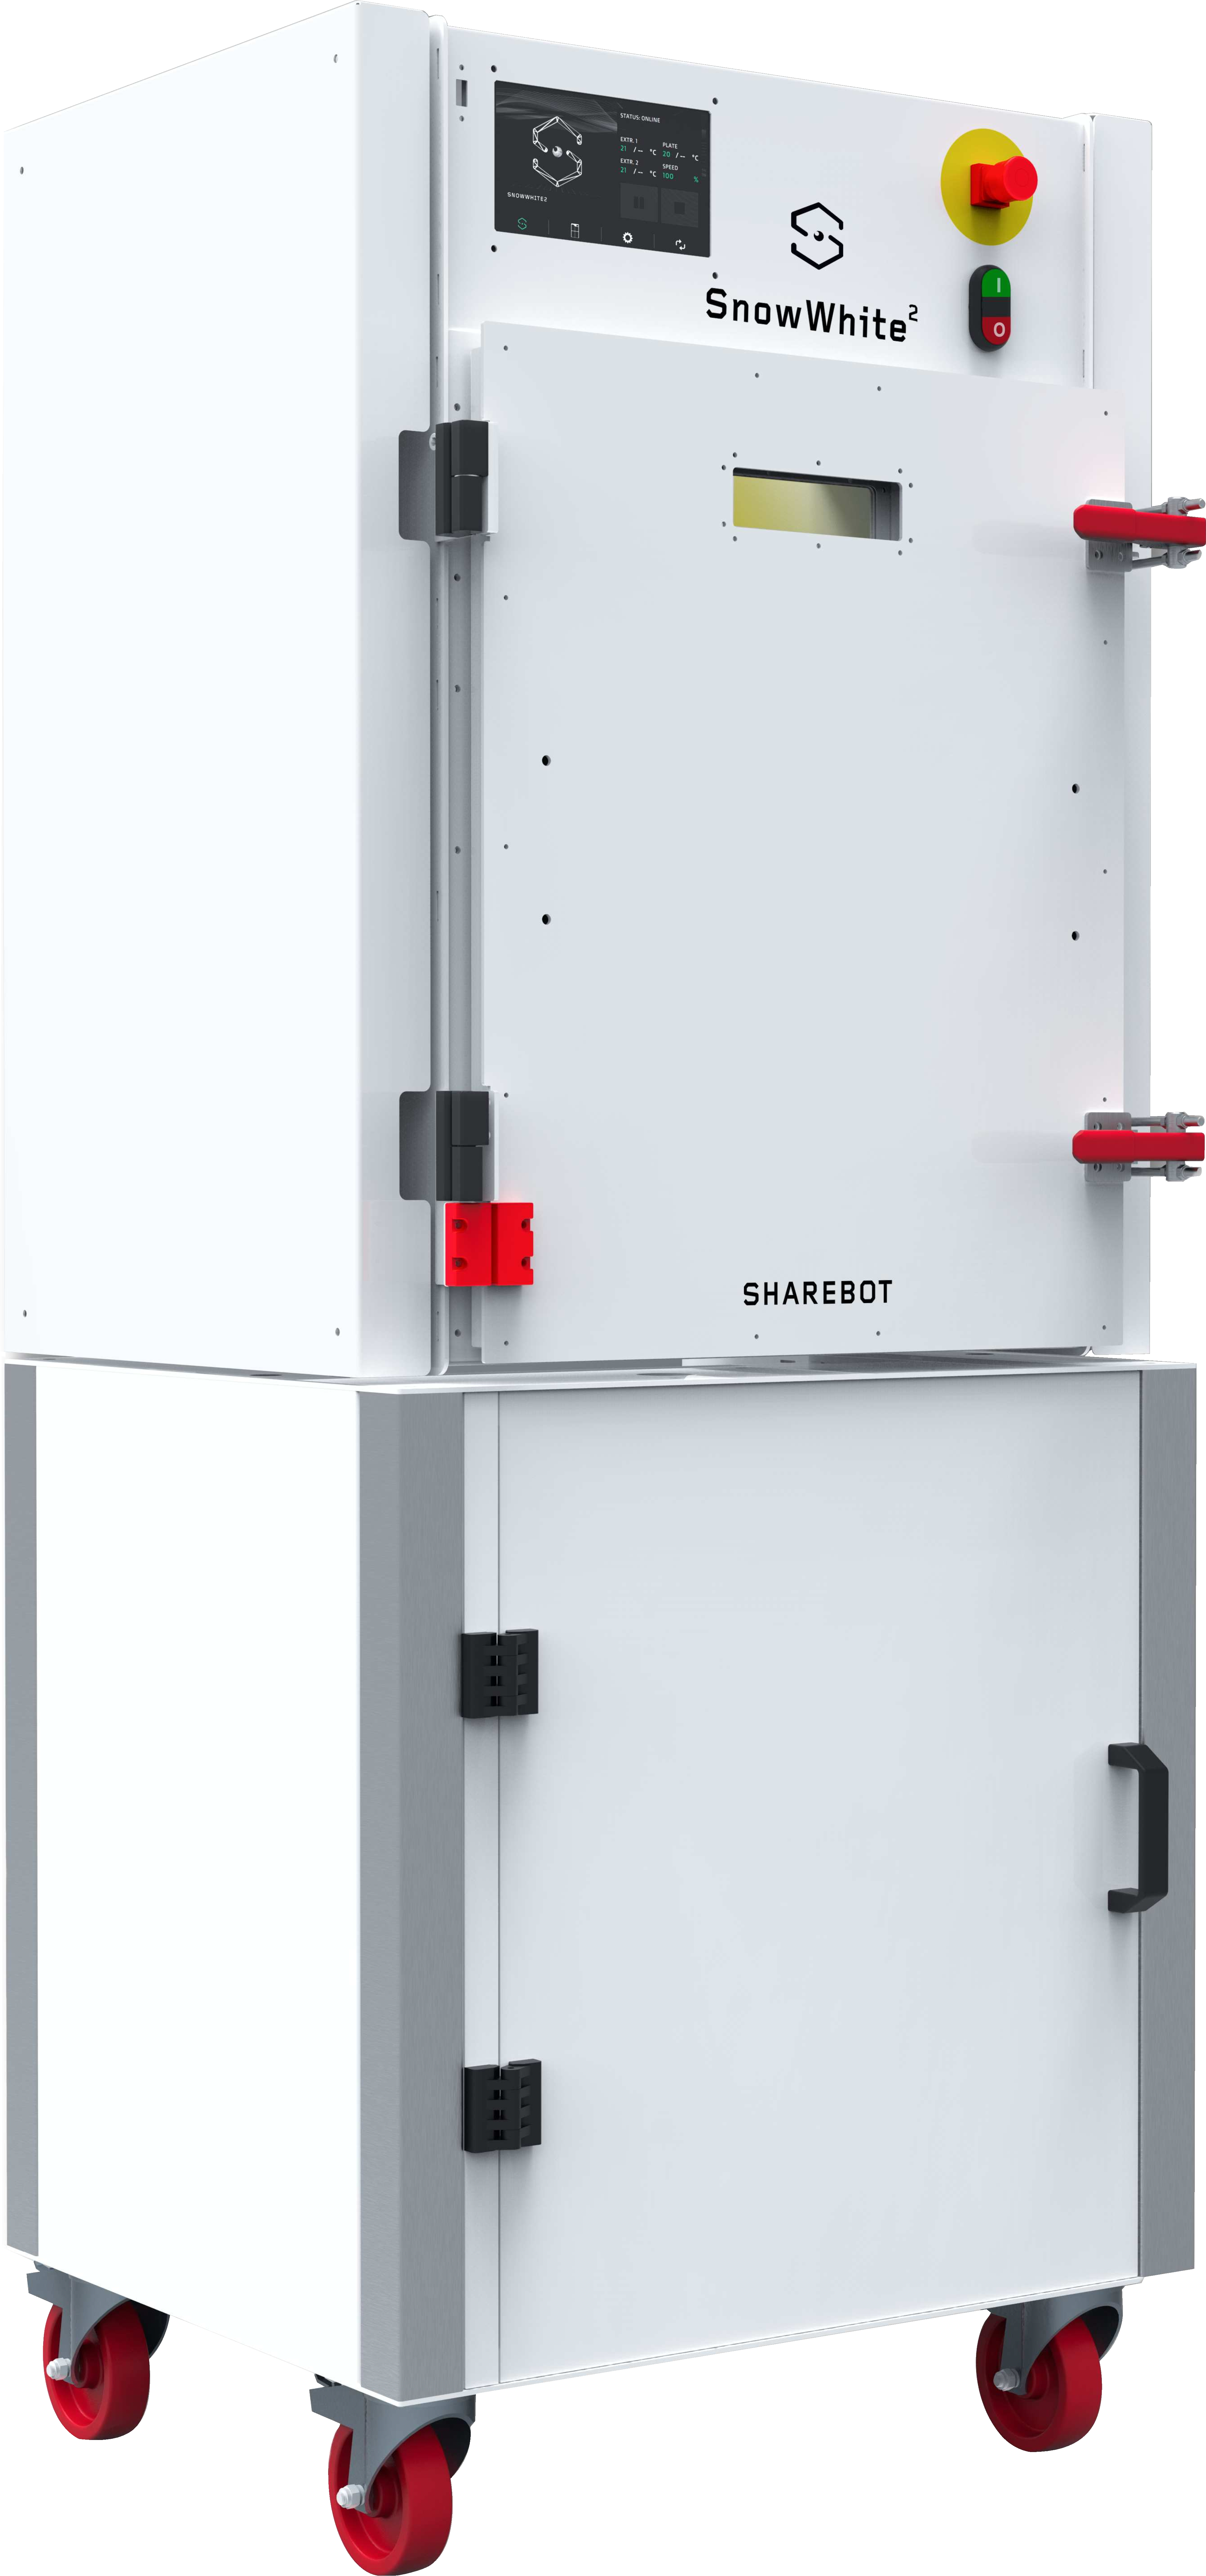
\includegraphics[width=0.5\textwidth]{Pictures/sharebot_snowhite2.eps}
            \caption{Sharebot Snowhite²}
            \label{fig:Sharebot_Snowhite2}
        \end{figure}

        The system is very modular and it features a standard powder distributor with a working area of 
        100x100x100 mm, but a reduced distributor with a 20x40x60 mm area has been used, given the available 
        quantity of PHBH powder.  \\ 

        The printer utilizes a CO2 laser with a 14 W maximum power output and a 10.6 µm wavelength. Power is controlled as 
        a percentage of its maximum output.  

        A value of 25 \% has been generally set for solid pieces, whereas a 30-35 \% range is preferred for pieces with extremely thin walls and intricate structures.  
        The power for the border has been set to a 5 \% increment with respect to the inner layers. \\ 

        The printer features a user friendly touch screen GUI, but all its features and logs can be accessed remotely for further control from any terminal.  

        The printer is equipped with a 3D camera, which allows to monitor the printing process in real time, 
        and to take pictures of the printed parts at every layer. \\

        \begin{figure}[h!]
            \centering
            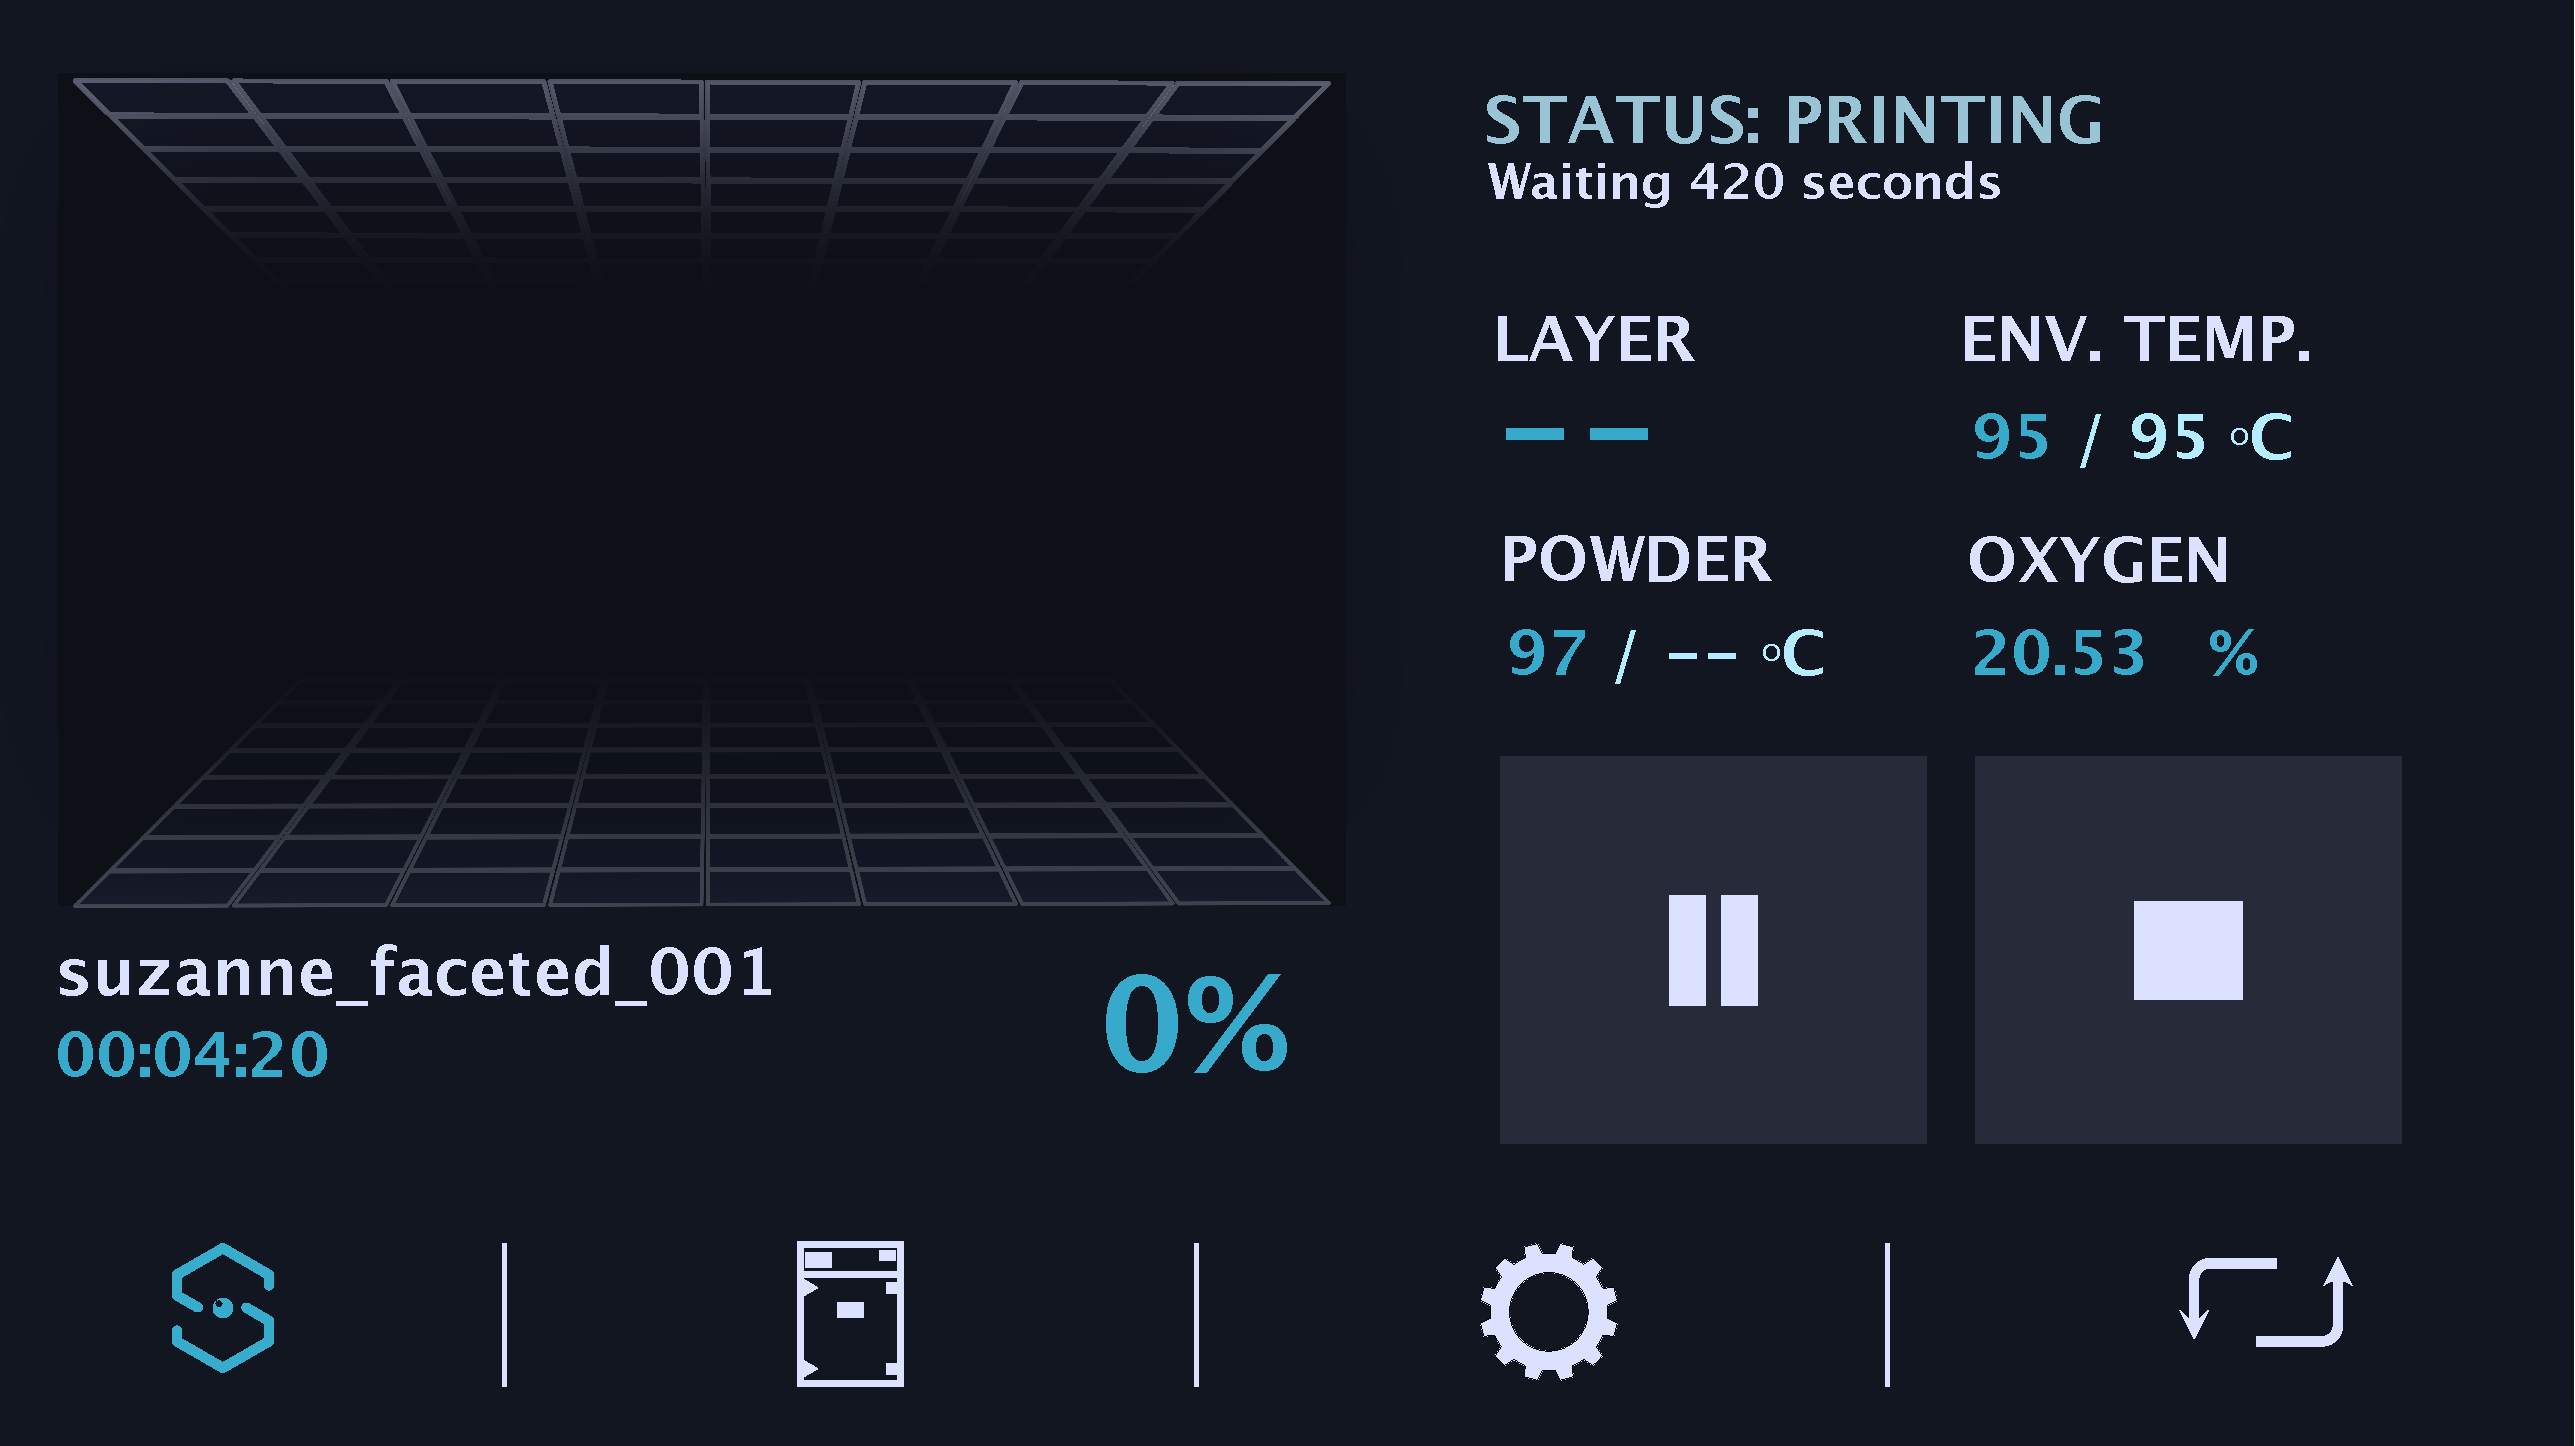
\includegraphics[width=\textwidth]{Pictures/Sharebot_GUI.pdf}
            \caption{Sharebot Snowhite² UI}
            \label{fig:Sharebot_UI}
        \end{figure}

        The polymer powder is distributed by a blade recoater, but a roller option is also available. 
        Air has been used for the printing process, but nitrogen or argon can be fed through the chamber, 
        should a modified atmosphere be needed.  \\

        The printer is also equipped with a powder recovery system, which allows to recover the powder 
        after the printing process, and to reuse it for further prints. \\ 

        The environment temperature has been set in a range of 85-95 $^oC$, with variable rates of success, 
        whereas values outside this threshold showcased critical issues, i.e. high porosity, sheeting and 
        delamination at low temperatures or adhesion to the recoater and consequent destruction of the printed specimen. \\ 

        Another configurable variable is laser hatching speed, which is measured relative to machine resolution, in dots/s, 
        which corresponds to 0.06 mm/s in metric units. 

        This has generally been kept at default values (40000 dots/s for the inner layers and 64000 dots/s for the border).  \\ 

        A maximum of three warming layers has been used for these prints, i.e. the powder is raised and warmed 
        up for three layers, without any laser hatching, to allow the powder to settle and to avoid 
        powder sheeting. \\ 
        A higher number of warming layers might be needed for larger prints, but it has not been tested 
        \ref{3D_model_creation}. \\

        Once the environment temperature has been set in the desired range (ideally within the theoretical 
        sintering window), the printer ramps it up in gradual steps, until the target is reached.  
        An additional waiting time of 120-300 s has been set after reaching the desired temperature, in order to let heat 
        uniformly distribute through the powder bed. \\

        The tank offset has been set prior to printing, depending on the desired print height or 
        layer number, which is calculated with the following formula: \\
        
        \begin{equation}
            Z =  \frac{1}{2} \cdot (0.3 \  N) \ \ \ \ \  [mm]
            \label{eq:layer_height}
        \end{equation}
        
        
        where:
        \begin{itemize}
            \item $Z$ is the tank offset, in mm
            \item $N$ is the number of layers to be printed 
            \item $0.3$ is the layer height, in mm, which is the default value for the \textit{Sharebot Snowhite²}
            \item $\frac{1}{2}$ is a correction factor, which is needed to account for the fact that the printing area is fed powder 
            from two side tanks.
        \end{itemize}
        



        \clearpage
        \subsection{Printed samples\label{Printed_samples}}

        Given the experimental nature of this work, several samples have been printed, with gradual 
        increases in complexity, in order to test the limits of the SLS workflow for the novel material. \\ 

        As earlier mentioned in \ref{Sharebot_Snowhite²}, the printer is modular and despite being equipped 
        with a default 100x100x100 mm working area, a reduced distributor with a 20x40x60 mm area has been used, 
        given the available quantity of PHBH powder. \\ 

        This setup is ideal for small scale prints, but as it will be shown later, the current results 
        are not exhaustively representative of the potential of the SLS workflow for PHBH. \\

        There are in fact intrinsic limitations to extremely small objects with intricate and fine details,
        especially at low z-height, which are related to both the material itself (as it is fragile and prone to 
        breaking) and the printing resolution of the SLS machine, which 
        did not seem to be able to print extremely small features with high fidelity to the original models. \\

        These limitations become less and less relevant with increasing z-height, as the part becomes 
        more robust, as well as with increasing overall size, where the printing resolution 
        is able to catch finer details with better accuracy. \\

        Nonetheless, the current results are still very promising, and they showcase the potential of the SLS workflow
        for PHBH, which can be further explored with larger prints, where the complexity of the models 
        can be pushed even further, as expected with SLS technology. \\  

        The first samples are simple geometries, which have been printed to test the feasibility of the SLS workflow 
        for PHBH. Square and rectangular prisms have been printed, with different z-heights, starting from single 
        layers, up to 15 layers, as a baseline for the following tests. \\ 

        The initial goal was in fact to find adequate printing parameters for the material, which required a lot 
        of trial and error, as the material is very sensitive to the printing conditions. \\

        The first prints have been made with a 25 \%  laser power setting, which has been found to be 
        a reasonable value for solid pieces, by visual inspection of single layers (which showcased 
        decent densification) and later confirmed by 
        mechanical testing on multilayer samples. 
        
        \clearpage

        %Some of the initial samples are showcased in the following figure: 
%
        %\begin{figure}[h!]
        %    \centering
        %    \includegraphics[width=0.2\textwidth]{Pictures/Printed_parts/benchmark_samples.eps}
        %    \caption{First printing attempts. Porosity and defects are more visible in the single layer samples.
        %    The rectangular prisms were the first to showcase a good level of densification and lack of deformation and 
        %    have been used as a baseline for the following tests.}
        %    \label{fig:printed_benchmarks}
        %\end{figure}

        As previously mentioned, the material is very sensitive to the printing conditions, and other than laser power,
        the environment temperature has been found to be the most critical parameter. \\ 

        After a long series of tests, the optimal temperature range has been found to be $85 \ ^oC$ - $95 \ ^oC$, which has been
        used for the following tests. \\ 

        It is important to note that the environment temperature is measured by a thermocouple, whereas the 
        powder bed temperature (which is a few degrees higher) is measured by an infrared sensor, which  
        is less accurate. 

        Therefore, these values might vary slightly for different machines, depending on how the different 
        temperatures are measured. \\ 

        The next step was to test the material with more complex geometries, which have been printed with the same 
        temperature range, but with a 30-35 \% laser power setting, which has been found to be optimal for the 
        emptier geometries, where heat is dissipated more easily, given the lower thermal mass. \\ 

        When dealing with thin, hollow and complex geometries, the most prominent issue is the tendency of the 
        blade recoater to stick to the printed piece and wipe the part out, which is a common 
        issue with SLS technology, and which 
        can be caused by different factors, such as the powder bed temperature, the laser power, the 
        environment temperature, the powder type and the powder distribution, among the many. \\ 

        Given the multifactorial and complex nature of the aforementioned issue, it is not possible to 
        pinpoint the exact cause of the problem, but it is possible to find a compromise between the 
        different parameters, which allows for a successful print. \\
        
        The introduction of other settings such as warming layers, pre-print 
        and between-layers waiting time, has been found to be useful in order to avoid 
        the blade recoater from wiping the part out. \\

        Using a roller recoater might also be a solution, but it has not been tested. \\ 

        The following printed specimens have been modeled as mentioned in \ref{3D_model_creation} and 
        have been catalogued with the following criteria: 

        \begin{equation}
            NN-SLS_{MM}
            \label{eq:SLS_specimen_notation}
        \end{equation}

        where: 

        NN is the number of layers and MM is the sequential number of the sample, respectively. \\ 

    \begin{table}[h!]
        \centering
        \resizebox{\textwidth}{!}{%
        \begin{tabular}{@{}cccccc@{}}
            \toprule
            \textbf{ID}        & \textit{Layers}  & \textit{Laser power {[}$\%${]}} & \textit{Environment temperature {[}$ ^{\circ}C${]}} \\ \midrule
            $15-SLS_{01}$      & 15               & 25                              & 90                                                  \\
            $15-SLS_{02}$      & 15               & 25                              & 95                                                  \\
            $55-SLS_{03}$      & 55               & 35                              & 95                                                  \\
            $01-SLS_{04}$      & 01               & 25                              & 85                                                  \\
            $50-SLS_{05}$      & 50               & 30                              & 90                                                  \\
            $10-SLS_{06}$      & 10               & 25                              & 90                                                  \\
            $15-SLS_{07}$      & 15               & 25                              & 90                                                  \\
            $15-SLS_{08}$      & 15               & 35                              & 87                                                  \\ \bottomrule
        \end{tabular}%           
        }
    \caption{A list of the most relevant 3D printed specimens}
    \label{tab:SLS_samples}
    \end{table}

        The printed parts showcase an excellent level of detail, which could potentially increase when printing larger objects. 
        Other than some superficial roughness and bumps, which are expected
        in most AM before surface treatments, the specimens are in a very good condition, with no visible cracks or other defects.
        The most significant specimens have been cut out from their photos and put against a pitch black background
        using \textit{Pixelmator Pro} \autocites{Pixelmator_Pro}, then assigned a size marker using \textit{Inkscape}
        \autocites{Inkscape}, as showcased in the following figures: 

        %\begin{figure}[h!]
        %    \centering
        %    \includegraphics[width=0.7\textwidth]{Pictures/Printed_parts/samples.eps}
        %    \caption{From top to bottom, clockwise: $15-dragonlogo_{filled}$, $15-hexagon_{filled}$, $55-octagonholes_{thin}$, 
        %    $50-boat_{thin}$, $10-DMA01_{filled}$, $01-square_{filled}$ (\ref{tab:SLS_samples}).}
        %    \label{fig:printed_specimens}
        %    % Indica quali nella caption, in base alla tabella
        %\end{figure}

        %\begin{figure}[h!]
        %    \centering
        %    \begin{subfigure}[a]{0.55\textwidth}
        %        \includegraphics[width=0.5\textwidth]{Pictures/Printed_parts/sample1-DMA-IMG_3178.eps}
        %        \subcaption{$10-DMA01_{filled}$ (\ref{tab:SLS_samples})}
        %        % Indica quale nella caption, in base alla tabella
        %    \end{subfigure}
        %        \vfill
        %    
        %    \begin{subfigure}[b]{0.5\textwidth}
        %        \centering
        %        \includegraphics[width=\textwidth]{Pictures/Printed_parts/sample3-DMA-IMG_3178.eps}
        %        \subcaption{$15-DMA02_{filled}$ (\ref{tab:SLS_samples})}
        %        % Indica quale nella caption, in base alla tabella
        %        \end{subfigure}
        %    \caption{Printed specimens used for DMA testing.}
        %    \label{fig:printed_specimens_DMA}
        %\end{figure}
%
        %\begin{figure}[h!]
        %    \centering 
        %    \begin{subfigure}[a]{0.41\textwidth}
        %        \includegraphics[width=\textwidth]{Pictures/Printed_parts/sample2-organicpattern.eps}
        %        \subcaption{$15-organicpattern_{thin}$, showcasing an intricate organic pattern (\ref{tab:SLS_samples}).}
        %        % Indica quale nella caption, in base alla tabella
        %    \end{subfigure}
        %        \vfill
        %    \begin{subfigure}[b]{0.5\textwidth}
        %        \centering
        %        \includegraphics[width=\textwidth]{Pictures/Printed_parts/sample4-octagon-holes-IMG_3181.eps}
        %        \subcaption{$55-octagonholes_{thin}$, showcasing an octagon with a circular array of octagon holes (\ref{tab:SLS_samples}).}
        %        % Indica quale nella caption, in base alla tabella
        %    \end{subfigure}
        %    \caption{Printed specimens with complex internal patterns.}
        %    \label{fig:printed_specimens_complex}
        %\end{figure}

        \begin{figure}[h!]
            \centering
            \includegraphics[width=\textwidth]{Pictures/Printed_parts/Fixed/DMA_samples.eps}
            \caption{DMA ready prismatic specimens $10-SLS_{06}$ (bottom) and $15-SLS_{07}$ (top).}
            \label{fig:printed_specimens_DMA}
        \end{figure}

        \begin{figure}[h!]
            \centering
            \includegraphics[width=\textwidth]{Pictures/Printed_parts/Fixed/filled_hexagon.eps}
            \caption{Specimen $15-SLS_{02}$, a filled hexagon.}
            \label{fig:printed_specimens_filledhexagon}
        \end{figure}

        \begin{figure}[h!]
            \centering
            \includegraphics[width=\textwidth]{Pictures/Printed_parts/Fixed/boat.eps}
            \caption{Specimen $50-SLS_{05}$, representing a boat model with curvature.}
            \label{fig:printed_specimens_boat}
        \end{figure}

        \begin{figure}[h!]
            \centering
            \includegraphics[width=\textwidth]{Pictures/Printed_parts/Fixed/organic_pattern_hexagon.eps}
            \caption{Specimen $15-SLS_{08}$, showcasing a complex internal pattern.}
            \label{fig:printed_specimens_organicpattern}
        \end{figure}

        \begin{figure}[h!]
            \centering
            \includegraphics[width=\textwidth]{Pictures/Printed_parts/Fixed/octagon_holes.eps}
            \caption{Specimen $55-SLS_{03}$, an octagon with a circular array of octagonal holes and a thin wall rim, with a total height of 55 layers.}
            \label{fig:printed_specimens_octagonholes}
        \end{figure}
        

        \clearpage

    
    \section{Conclusions\label{conclusions}}

    As stated in the \textit{Thesis Goal} \ref{Thesis_Goal}, the aim of this work was to investigate the feasibility of PHBH as a 
    material for additive manufacturing, with a particular focus on the SLS process. \\ 

    The entire work has been very experimental and innovative in nature, as it is the first time that a novel bio-based polymer such as PHBH has been investigated 
    for the aforementioned use and brought to the point of being printable with SLS. \\
    
    The approach has been exploratory and yet successful in all of its phases, starting from the powder production and characterization, all the way to the successful 
    SLS printing of the material, which leaves even more room for further research and development. 
    

    \clearpage
    \section{Future development\label{Future_development_and_research}}

    The entire project has been carried out with an experimental approach and, despite poor direct support 
    from the currently available literature, a better understanding of 
    the material and its behavior has emerged, but the need for further research and development is still 
    present. \\ 

    Starting from the powder production pipeline, the results have already been excellent (as showcased in chapters \ref{recipe_improvement}, \ref{Initial_recipe}, 
    \ref{consistent_reproducibility}) with the available notions and tools, bringing the pellet to powder yield to 
    a very significant increase. \\ 

    However, the process is still in its infancy, and the entire premise of the project is to develop a sustainable 
    and cost-effective production pipeline, which is not only able to produce a high-quality powder, but also 
    to do so in a way that is environmentally friendly. Therefore, the next step is to find a way to reproduce and 
    even improve the results obtained with the current recipe, but in a more sustainable way, by further 
    investigating the use of alternative solvents. \\ 

    Another possibility is to find a way to retrieve the evaporated chloroform, assuming an effective solvent recovery 
    system is available and cost-effective. \\ 

    The next step is to further investigate the use of the powder in the SLS process, by further optimizing the 
    printing parameters, the powder granulometry and morphology and experimenting with different additives or material blends that 
    could improve the mechanical properties of the material, as well as investigating the possibility of enhancing the printed parts 
    with post-processing techniques. \\ 


    \clearpage


    \printbibliography
\end{document}